% LayerFS paper draft.
% Status: Research; informative and not a product contract.
% Build: latexmk -pdf layerfs.tex
\documentclass[letterpaper,twocolumn,10pt]{article}
\usepackage[margin=0.75in,columnsep=0.33in]{geometry}
\usepackage{mathptmx}
\usepackage[T1]{fontenc}
\usepackage{microtype}
\usepackage{booktabs}
\usepackage{xcolor}
\usepackage{graphicx}
\usepackage{enumitem}
\usepackage{balance}
\usepackage{tikz}
\usetikzlibrary{positioning,arrows.meta,fit,shapes.geometric,calc,decorations.pathreplacing}
\usepackage{pgfplots}
\pgfplotsset{compat=1.17}
\usepackage[hidelinks]{hyperref}
\usepackage{algorithm}
\usepackage{algpseudocode}
\usepackage{bytefield}
\usepackage{url}
\usepackage{longtable}
\usepackage{amsmath}

\setlist{nosep,leftmargin=*}
\newif\ifdraft\drafttrue
\newcommand{\dnote}[1]{\ifdraft\textcolor{red!70!black}{\textsf{\small[#1]}}\fi}
\newcommand{\sys}{LayerFS}
\newcommand{\ws}{Workspace}
\newcommand{\X}{$\times$}

\title{\sys{}: A Recursive Filesystem for\\ Ephemeral Computing in AI Agents}
\author{Draft --- authors withheld}
\date{}

\begin{document}
\maketitle

\begin{abstract}
AI coding agents spend most of their time thinking, not running: in 2,095
agent sessions we analyzed, the model takes a median 84\% of active time,
and most tool calls only touch files. Yet each agent is given a whole
computer for its task, and that computer's disk is the only copy of its
work. \sys{} inverts the arrangement with \emph{ephemeral computing}:
compute is borrowed per command, and all state lives outside it, in one
shared, versioned Store.
File calls run in the agent's own process against it and need no computer.
Each shell call mounts a complete, writable \ws{}---source, \texttt{.git},
installed dependencies, build outputs and every ignored file---over an
immutable committed root, in time independent of tree size; it commits what
changed and goes away. Every step becomes an immutable commit, and the
filesystem is \emph{recursive}: any commit, including one inside a fork of
a fork, can start a new Branch at the same constant cost, without copying
data.

Recording whole trees at every step is affordable because commits share
structure. In a 13-hour build by nine agents, 4,354 commits of a 9\,GB tree
on 211 Branches occupy 4.93\,GB---less than half of one checkout of the
final tree---and the median edit commit adds 0.9\,KB. Mounts take a median
7\,ms and forks 5\,ms. We find that commit granularity decides which storage
mechanism matters: per-call commits make exact deduplication dominant,
while coarse snapshots rely on delta compression. Against ovnfs, an overlay
filesystem for agent checkouts, \sys{} adds 6--22\X{} fewer bytes per
commit on code histories and commits 1.5--21\X{} faster from a cold cache;
it is slower on cold large-file reads, bulk import and brand-new data.
\end{abstract}

\section{Introduction}

An AI coding agent works in a loop: the model reads context and decides on
an action, a tool executes it, and the result returns to the model. Most
tool calls read or edit files; a minority run commands that need an
operating system---building, testing, installing packages. In 2,095 agent
sessions we analyzed, the model accounts for a median 84\% of each
session's active time, and about 63\% of file and shell calls are file
operations that need no process at all (\S\ref{sec:premise}).

Today's agent infrastructure nevertheless starts from the computer. Each
task receives a sandbox---a container~\cite{e2b} or a micro-VM~\cite{firecracker}---whose
local filesystem holds the repository, its installed dependencies and every
intermediate result. The sandbox must stay alive for the whole task because
its disk \emph{is} the agent's state. This couples three things that have
different lifetimes: the agent's files (which must survive the task, be
inspected, branched and resumed), the compute that runs a command (needed
for seconds), and the model's thinking time (minutes, needing no compute at
all). It also makes checkpointing, branching and parallel exploration
expensive: copying or snapshotting a sandbox costs seconds and gigabytes,
and Git-based alternatives drop the ignored files---\texttt{node\_modules},
build outputs, caches---so every fresh checkout must reinstall before it can
run anything.

We present \sys{}, a filesystem for \textbf{ephemeral computing}: compute
is borrowed per command and given back, and state lives outside it, in
durable history that every agent shares. Each agent mounts a complete,
writable \ws{} over shared committed history, does its work, commits what it
changed, and goes away. \sys{} is also \textbf{recursive}: every step is a
commit, and any commit---including one inside a fork of a fork, or in the
middle of an earlier rollout---can start a new Branch at the same constant
cost. The two halves, ephemeral \ws{}s and durable shared history, have
different jobs.

\emph{Ephemeral Workspaces} are the compute side, borrowed per command:
\begin{itemize}
\item \textbf{File calls need no computer.} Reads, writes and edits run in
  the agent's process, directly against the Store; each write is one atomic
  commit (\S\ref{sec:filecalls}).
\item \textbf{Shell calls get a \ws{}.} A \ws{} is a complete POSIX view of a
  Branch, including dependencies, build outputs and ignored files. Mounting
  scans, copies and installs nothing; its only new file is a small private
  overlay database (\S\ref{sec:mount}). After the command, a commit records
  every change regardless of which process made it, and unmount discards the
  view (\S\ref{sec:commit}).
\end{itemize}

\emph{Durable shared history} is the state side. It outlives every \ws{},
Sandbox and agent, and every agent, Branch and project on a Store shares it:
\begin{itemize}
\item \textbf{Every step is a commit} that can be read, diffed or blamed.
\item \textbf{Forks are recursive.} Any commit, at any fork depth, can start
  a Branch by writing one metadata row, so rollouts, best-of-$N$ sampling~\cite{monkeys} and tree
  search~\cite{tot,uct} become cheap filesystem operations; every step of a
  rollout is itself a node to search from (\S\ref{sec:fork},
  \S\ref{sec:search}).
\item \textbf{Many agents can work on one Branch}, with conflicting writes
  refused atomically rather than silently interleaved (\S\ref{sec:merge}).
\end{itemize}

\textbf{Recording everything must be nearly free}, or none of this is
practical: every commit names a whole tree, build outputs included. \sys{}
shares first and compresses second. Unchanged subtrees keep their
identities, so a commit costs what changed; content addressing reuses
identical files and chunks across steps, Branches and projects; and what
remains new is delta-encoded against a base chosen from filesystem events
such as rename-over saves, then compressed (\S\ref{sec:storage}).

The individual storage techniques---content-defined chunking~\cite{lbfs,fastcdc},
content addressing~\cite{venti,git}, resemblance-based delta
compression~\cite{shilane,finesse}---are well known; backup systems and
version-control systems apply them \emph{offline}, over complete snapshots.
\sys{} applies them \emph{online}, inside a live filesystem's commit path,
at tool-call latency, and organizes agent execution around the result. Doing
so exposes a finding we did not expect: \emph{commit granularity decides
which mechanism saves space}. With one commit per tool call, consecutive
states are nearly identical and exact deduplication carries the load
(1,179\X{} against 5.4\X{} from deltas and compression in a nine-agent run);
with coarse snapshots the burden shifts to delta encoding.

This paper makes the following contributions:
\begin{itemize}
\item A characterization of where agent time and tool calls go, from 2,095
  sessions across two agent systems (\S\ref{sec:premise}).
\item The ephemeral-\ws{} model: complete views whose mount cost is
  independent of tree size and whose commit cost follows the change, over
  recursive history in which any commit, at any fork depth, can be forked
  (\S\ref{sec:design}--\S\ref{sec:history}).
\item A Store that builds and encodes immutable objects in parallel and
  serializes metadata publication through one writer with short holds, so many \ws{}s and in-process
  callers share one database (\S\ref{sec:store}).
\item An online storage pipeline---structural sharing first, then delta
  bases chosen from filesystem events---and the observation that commit
  granularity decides which of the two matters (\S\ref{sec:storage},
  \S\ref{sec:eval-granularity}).
\item An evaluation including a 13-hour, nine-agent build and comparisons
  with an agent overlay filesystem, Btrfs snapshots and Git, including the
  cases where \sys{} loses (\S\ref{sec:eval}).
\end{itemize}

\section{Agents Think More Than They Run}
\label{sec:motivation}

\subsection{How agents use computers}
\label{sec:premise}

To ground the design we analyzed agent runs recorded on one developer's
machine: 483 sessions of an open-source agent harness driving six model
families (49,757 agent steps, 251 hours inside steps), and 1,612 transcripts
of a commercial coding agent (14,641 prompts, 1,043 active hours, with time
spent waiting for the human excluded). Table~\ref{tab:premise} summarizes
them.

\begin{table}[t]
\centering
\small
\setlength{\tabcolsep}{3pt}
\begin{tabular}{l r r}
\toprule
& Harness & Coding agent \\
\midrule
Sessions / transcripts & 483 & 1,612 \\
Model share of active time, aggregate & 64.3\% & 68.9\% \\
\quad per session, median & 85\% & 84\% \\
Tool result $\rightarrow$ next call, median & 6.5\,s & 5.6\,s \\
File + shell calls & 61,001 & 211,613 \\
\quad file operations (any tool) & 63.3\% & 61.9\% \\
\quad need process execution & 33.5\% & 31.6\% \\
Shell commands that only read/search & 52.4\% & 53.5\% \\
Shell calls per prompt, median / mean & 3 / 21.8 & 2 / 12.9 \\
\bottomrule
\end{tabular}
\caption{Where agent time and tool calls go. ``File operations'' counts
dedicated file tools plus shell commands whose program reads, searches or
moves files; the rest builds, tests, runs programs, writes Git state or
manages infrastructure.}
\label{tab:premise}
\end{table}

\begin{figure}[t]
\centering
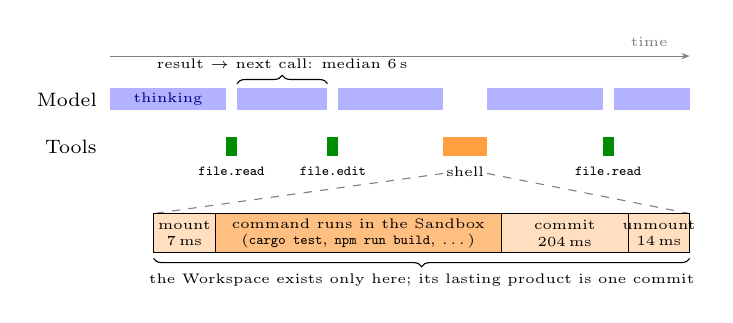
\begin{tikzpicture}[font=\scriptsize,x=0.92cm,y=1cm]
\node[anchor=east] at (-0.05,1.0) {Model};
\node[anchor=east] at (-0.05,0.4) {Tools};
\foreach \a/\b in {0/1.6, 1.75/3.0, 3.15/4.6, 5.2/6.8, 6.95/8.0}
  \fill[blue!30] (\a,0.86) rectangle (\b,1.14);
\node[font=\tiny,blue!50!black] at (0.8,1.0) {thinking};
\foreach \a/\t in {1.6/read, 3.0/edit, 6.8/read} {
  \fill[green!55!black] (\a,0.28) rectangle ++(0.15,0.24);
  \node[font=\tiny,anchor=north] at (\a+0.075,0.27) {\texttt{file.\t}};
}
\fill[orange!75] (4.6,0.28) rectangle (5.2,0.52);
\node[font=\tiny,anchor=north] at (4.9,0.27) {shell};
\draw[decorate,decoration={brace,amplitude=3pt}] (1.75,1.2) -- node[above=2pt,font=\tiny]
  {result $\rightarrow$ next call: median 6\,s} (3.0,1.2);
\draw[-{Stealth[length=3pt]},gray] (0,1.55) -- node[above,font=\tiny,pos=0.93]{time} (8.0,1.55);
% zoom into the shell call
\draw[dashed,gray] (4.6,0.06) -- (0.6,-0.45);
\draw[dashed,gray] (5.2,0.06) -- (8.0,-0.45);
\draw[fill=orange!25] (0.6,-0.95) rectangle (1.45,-0.45);
\node[align=center,font=\tiny] at (1.025,-0.7) {mount\\7\,ms};
\draw[fill=orange!50] (1.45,-0.95) rectangle (5.4,-0.45);
\node[align=center,font=\tiny] at (3.425,-0.7) {command runs in the Sandbox\\(\texttt{cargo test}, \texttt{npm run build}, \dots)};
\draw[fill=orange!25] (5.4,-0.95) rectangle (7.15,-0.45);
\node[align=center,font=\tiny] at (6.275,-0.7) {commit\\204\,ms};
\draw[fill=orange!25] (7.15,-0.95) rectangle (8.0,-0.45);
\node[align=center,font=\tiny] at (7.575,-0.7) {unmount\\14\,ms};
\draw[decorate,decoration={brace,amplitude=3pt,mirror}] (0.6,-1.02) -- node[below=2pt,font=\tiny]
  {the \ws{} exists only here; its lasting product is one commit} (8.0,-1.02);
\end{tikzpicture}
\caption{One agent turn, schematically. The model thinks most of the time
(median 84--85\% per session, Table~\ref{tab:premise}). File calls write to
the Store from the agent's process and need no computer. Only a shell call
borrows a \ws{}, for the length of one command; latencies are medians from
the nine-agent build (Table~\ref{tab:quarry-lat}).}
\label{fig:turn}
\end{figure}

Two observations follow. \textbf{Most time is spent in the model.} In
aggregate the model accounts for 64--69\% of active wall time, and in the
median session for 84--85\%; the median gap between a tool's result and the
next tool call is about six seconds. A computer held for the task idles
through all of it. \textbf{Most tool calls need no computer.} Agents issue
most calls \emph{as} shell commands---the coding agent chose its shell tool
for 89\% of file and shell calls even though it also offers file
tools---but more than half of those commands only read or search files.
Counting dedicated file tools, 62--63\% of calls are file operations that a
filesystem API can serve directly; about a third need to run a process.
Figure~\ref{fig:turn} shows what this means for one turn: a computer is
needed for a few short intervals, not for the whole task.

These numbers come from one developer's systems-heavy work, which inflates
build and test time, and we classify shell commands by their first program
word. They are indicative, not general; \S\ref{sec:discussion} lists what a
cleaner measurement would record.

\subsection{The cost of a computer per agent}

A sandbox held for a whole task pays for idle time while the model thinks,
and it is the sole home of the agent's work: losing it loses the state, and
branching it means copying it. Two common ways to avoid holding a sandbox
both fall short.

\textbf{Re-create from Git.} Cloning or checking out a commit is cheap only
because Git ignores the files that make a tree runnable: installed
dependencies, build outputs and caches. A fresh checkout must reinstall
before the first test can run, a cost measured in minutes for typical
JavaScript or Rust projects. Git also commits by scanning the working tree,
and it is not a mountable filesystem.

\textbf{Snapshot the sandbox.} Container layers, VM snapshots and
copy-on-write file systems capture everything, but at whole-file or
whole-image granularity, or only for in-place updates. Overlay filesystems
copy a file up in full on its first write~\cite{overlayfs}. Snapshot
filesystems such as Btrfs~\cite{btrfs} share extents that stay in place, but
a file rewritten whole---as editors, Git and package managers do when they
write a temporary file and rename it over the original---is new data.

\subsection{Agent filesystems today}

Several systems target agents directly. ovnfs~\cite{ovnfs} provides
disposable, Git-integrated agent checkouts through file-level copy-on-write
overlays with snapshots into a packed object store. AgentFS~\cite{agentfs}
stores a filesystem in SQLite as fixed 4\,KiB chunk rows with a per-session
delta database, but (in the version we studied, 0.6.4) keeps no version
history or snapshots. JuiceFS~\cite{juicefs} and earlier database-backed
filesystems~\cite{inversion,tablefs} keep metadata in a database but are not
versioned. None combines a complete mountable tree, per-call history and
fork-from-anywhere at low storage cost.

\subsection{Goals}

\begin{enumerate}
\item \textbf{Complete views.} A \ws{} is the whole tree, ignored files
  included, so commands run as in an installed checkout.
\item \textbf{Constant-cost bootstrap.} Mounting does not scan, copy or
  install; cost is independent of tree size.
\item \textbf{Commit cost follows the change}, not the size of the tree or
  of the edited file.
\item \textbf{Every step is history.} Every tool call that changes the tree
  is an immutable, forkable commit.
\item \textbf{Affordable history.} Storage grows with what changed, across
  steps, Branches and projects.
\item \textbf{Shared without a server.} Many processes and \ws{}s share one
  Store with no database server in the data path.
\end{enumerate}

\section{Ephemeral Workspaces, Shared History}
\label{sec:design}

\begin{figure}[t]
\centering
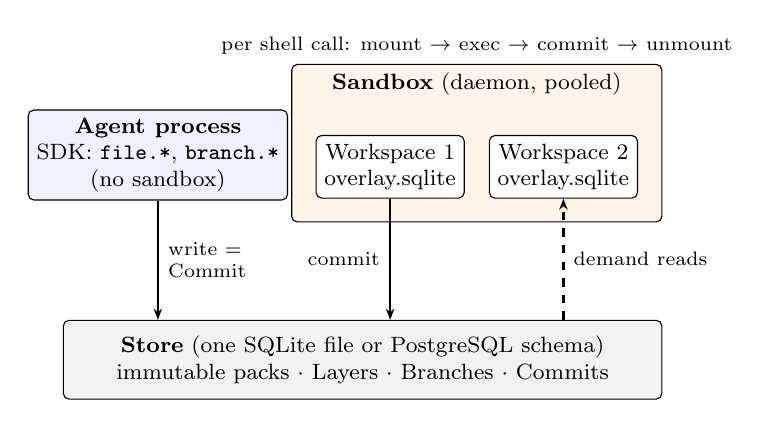
\begin{tikzpicture}[
  font=\footnotesize,
  box/.style={draw,rounded corners=2pt,align=center,inner sep=3pt},
  arr/.style={-{Stealth[length=4pt]},thick}]
\node[box,minimum width=7.6cm,minimum height=1.0cm,fill=gray!10] (store) at (0,0)
  {\textbf{Store} (one SQLite file or PostgreSQL schema)\\
   immutable packs $\cdot$ Layers $\cdot$ Branches $\cdot$ Commits};
\node[box,fill=blue!6,minimum width=2.4cm] (agent) at (-2.6,2.6)
  {\textbf{Agent process}\\SDK: \texttt{file.*}, \texttt{branch.*}\\(no sandbox)};
\node[box,fill=orange!8,minimum width=4.7cm,minimum height=2.0cm] (sbx) at (1.45,2.75) {};
\node[anchor=north,inner sep=3pt] at (sbx.north) {\textbf{Sandbox} (daemon, pooled)};
\node[box,fill=white] (w1) at (0.35,2.45) {\ws{} 1\\overlay.sqlite};
\node[box,fill=white] (w2) at (2.55,2.45) {\ws{} 2\\overlay.sqlite};
\draw[arr] (agent.south) -- node[right,align=left,font=\scriptsize]{write =\\Commit} (agent.south|-store.north);
\draw[arr] (w1.south) -- node[left,font=\scriptsize]{commit} (w1.south|-store.north);
\draw[arr,dashed] (w2.south|-store.north) -- node[right,font=\scriptsize]{demand reads} (w2.south);
\node[align=center,font=\scriptsize,anchor=south] at (sbx.north)
  {per shell call: mount $\rightarrow$ exec $\rightarrow$ commit $\rightarrow$ unmount};
\end{tikzpicture}
\caption{\sys{} architecture. State lives only in the Store. File calls run
in the agent's process. Shell calls borrow a \ws{}: a private overlay over a
committed root, created at mount and deleted at unmount.}
\label{fig:arch}
\end{figure}

\paragraph{Objects.} A \emph{project} is one source tree. Its committed
state lives in a \emph{Store}: one SQLite database file in WAL mode, or one
PostgreSQL schema, holding immutable content-addressed objects and the
history records that name them. A \emph{Branch} is a named line of
\emph{Commits}; each Commit names a filesystem root and its parent(s). The
distinguished Branch \texttt{main} is read-only and grows by \emph{Layers},
each a published state. Project initialization reads the source tree once,
including \texttt{.git}, dependencies, caches, symlinks and every
Git-ignored file, and makes it the first Layer.

\paragraph{Two execution paths.} Figure~\ref{fig:arch} shows the two ways an
agent touches state. \emph{File calls} (\texttt{file.read}, \texttt{file.write},
\texttt{file.edit}, and history calls such as \texttt{branch.fork} or
\texttt{file.blame}) run inside the caller's process, which opens the Store
directly. \emph{Shell calls} run in a \emph{Sandbox}: a long-lived daemon
plus an isolation environment (Linux namespaces and cgroups inside a VM or
container, or a host process on macOS). The orchestrator mounts a Branch as
a \ws{} in the Sandbox, runs the command, commits and unmounts.

\paragraph{What is ephemeral.} The unit created and destroyed per call is
the \ws{}---a private overlay database plus a kernel mount---not the Sandbox.
A Sandbox holds up to 16 \ws{}s, shares an object cache among them, and can
be discarded at any time: it never holds committed state, so losing it loses
only uncommitted overlays, and any Sandbox attached to the Store can mount
any Branch. This is what lets compute be pooled, replaced and scaled
independently of the agents whose state it serves.

\paragraph{What is durable.} History---every object, Commit, Branch and
Layer---lives only in the Store and is never rewritten. By \emph{durable}
we mean that it outlives every \ws{}, Sandbox and agent: losing any of them
loses no committed work. We do not mean crash-durable in the
\texttt{fsync} sense; the Store trades that for latency
(\S\ref{sec:durable}).

\paragraph{Interface.} One call table defines the whole interface: 73 calls
in ten families, from which the \texttt{layerfs} command line and the Node
and Python SDKs are generated, so \texttt{layerfs.file.write} in an SDK is
\texttt{layerfs file write} in a shell. Table~\ref{tab:api} groups the calls
an agent uses by the role they play; Appendix~\ref{app:cli} lists all of them.

\begin{table}[t]
\centering
\footnotesize
\begin{tabular}{@{}p{0.27\columnwidth}p{0.69\columnwidth}@{}}
\toprule
Role & Calls \\
\midrule
No computer: file calls, one Commit per write &
\texttt{file.read}, \texttt{write}, \texttt{edit}, \texttt{apply}, \texttt{cp},
\texttt{mv}, \texttt{rm}, \texttt{mkdir}, \texttt{stat}, \texttt{list},
\texttt{glob}, \texttt{grep} \\
\addlinespace
Borrowed compute: one shell call &
\texttt{workspace.mount}, \texttt{exec}, \texttt{commit}, \texttt{unmount};
\texttt{workspace.status}, \texttt{exec\_cancel} \\
\addlinespace
Compute pool &
\texttt{sandbox.create}, \texttt{close}, \texttt{get}, \texttt{list};
\texttt{machine.*} \\
\addlinespace
Recursive forks &
\texttt{branch.fork} (from any Branch, Commit or Layer), \texttt{merge},
\texttt{publish} \\
\addlinespace
Every step a checkpoint &
\texttt{commit.list}, \texttt{get}, \texttt{diff}; \texttt{branch.diff},
\texttt{commits}; \texttt{file.blame}, \texttt{revision}, \texttt{diff};
\texttt{file.read} at a Commit \\
\addlinespace
Shared state &
\texttt{store.create}, \texttt{connect} (PostgreSQL), \texttt{push},
\texttt{attach}; \texttt{project.init}, \texttt{export} \\
\addlinespace
Measurement &
\texttt{store.stats}, \texttt{project.stats},
\texttt{branch.commits --include-storage} \\
\bottomrule
\end{tabular}
\caption{The \sys{} 2.0 interface by role. A call written after a family
name belongs to that family (\texttt{write} is \texttt{file.write}).}
\label{tab:api}
\end{table}

\section{Ephemeral Workspaces}
\label{sec:workspaces}

\subsection{File calls without a computer}
\label{sec:filecalls}

A file call binds a private \ws{} that is never mounted. Its overlay is a
copy of the process's template; the call applies each change as overlay
jobs and then commits through exactly the same capture, construction, merge
and publication path as a mounted \ws{} (\S\ref{sec:commit}). A write is
therefore one atomic operation and one Commit. A write that leaves the tree
unchanged answers \texttt{UpToDate} and creates nothing. Because the caller
opens the Store itself, there is no server in the data path.

Opening a SQLite Store from several processes requires one kernel and a
local filesystem whose locking SQLite trusts (ext4, xfs or btrfs on Linux;
APFS on macOS); a guard refuses anything else as \texttt{Unsupported}. Hosts
that cannot open the Store directly forward each call once, with no retry
or replay, to a loopback worker on the Store's machine. With the PostgreSQL
backend, callers on different machines can open one Store, since
PostgreSQL arbitrates access instead of the local kernel.

\subsection{Constant-cost mount}
\label{sec:mount}

Mounting a Branch performs four steps: read the Branch's head from the
Store, decode and authenticate the root object, copy a pre-built,
schema-only overlay template into a fresh SQLite file, and attach a FUSE
session (Linux) or a loopback NFSv3 export (macOS). None of these steps
depends on the size of the tree: nothing is scanned, copied, restored or
installed. Directory pages, inode-table pages and file extents are fetched
on demand from the Store when first accessed, authenticated against their
object identifiers, and kept in a per-daemon cache keyed by identity and
shared by all \ws{}s of that daemon. The first read of a file still pays
real I/O; what mount avoids is work proportional to the tree.

\subsection{A private overlay per \ws{}}
\label{sec:overlay}

Each mounted \ws{} owns one SQLite overlay database configured for speed
over durability (in-memory journal, \texttt{synchronous=OFF}, exclusive
locking, in-memory temporary storage). It records only changes: names and
whiteouts, inodes, and file bytes as 4\,KiB cells and 32\,KiB dense runs.
\emph{Reference pieces} describe ranges equal to already-committed bytes
without copying them, so a small write to a large file stores only what was
written. Open-file, directory-position and kernel-reference state live in
daemon memory.

One lock guards a \ws{}'s connection. It is held for exactly one short
atomic job---at most one transaction---and never across Store I/O, a command
or a commit. Every job is bounded by a window (FUSE writes and reads of at
most 128\,KiB, 256\,KiB transfers on the NFS route, 1,024-row pages), so no file, edit or \ws{} size is capped by
resident memory. Workspaces share no overlay connection, writer, page cache
or memory budget; the only shared state is committed immutable content and
the Store.

FUSE kernel write-back caching is disabled: every \texttt{write(2)} is
published to the overlay before it returns. This makes capture exact---an
acknowledged write is always in the next commit---at the price of writing
new data through SQLite at write time (\S\ref{sec:eval-slow}).

\paragraph{Execution is not the filesystem's business.} Any process that
can see the mount uses ordinary system calls. The daemon supervises no
commands and registers no executions; the Sandbox runtime launches commands,
owns their streams and exit status, and places each in its own cgroup. A
commit captures what was published, not what a registered command did.

\subsection{Commit cost follows the change}
\label{sec:commit}

A commit proceeds in five steps.
\begin{enumerate}
\item \textbf{Capture.} The overlay's active generation is sealed as the
  published frontier and a new one opens. No rows are copied and nothing is
  filtered by process: changes from several commands, including background
  processes, are captured together.
\item \textbf{Construct.} One producer thread reads only the sealed rows and
  the immutable base. Unchanged directories keep their stored roots. A
  changed file applies localized edits to its extent tree: it splits stored
  extents at edit boundaries, chunks only the new bytes and rebuilds only
  the pages on the paths to the root (\S\ref{sec:edits}). A file recreated
  with identical bytes reuses its stored root.
\item \textbf{Merge.} If the Branch head moved since the \ws{}'s base, the
  candidate is merged three-way with the new head before publication.
\item \textbf{Publish.} A short \emph{publication lane}, holding the
  Store's single writer, re-checks the head, merges whatever landed in the
  meantime (bounded) and advances the Branch in one transaction.
\item \textbf{Install.} The \ws{}'s base is rebound to the new root without
  a tree walk; changes made after the capture remain on top.
\end{enumerate}
A commit with no changes answers \texttt{UpToDate} without capturing,
saving or taking the lane.

Commit captures a filesystem, not a process. Unflushed dirty
\texttt{mmap} pages and writes by still-running descendants that have not
reached the overlay are not captured; command exit is not treated as proof
that a command's descendants are finished.

\subsection{Unmount and reclamation}

Unmount refuses a \ws{} with uncommitted changes unless told to discard
them. It then detaches the kernel mount, drains in-flight requests, revokes
kernel references and deletes the overlay file as a whole. Committed history
is untouched. A \ws{} is therefore a disposable view whose only lasting
product is a commit.

\section{Shared History}
\label{sec:history}

History is the half of \sys{} that lasts. Every agent, Branch and project
on a Store shares one object graph and one record of Commits and Layers, so
forking, merging and many agents working at once are operations on
metadata.

\subsection{Recursive forks}
\label{sec:fork}

\begin{figure}[t]
\centering
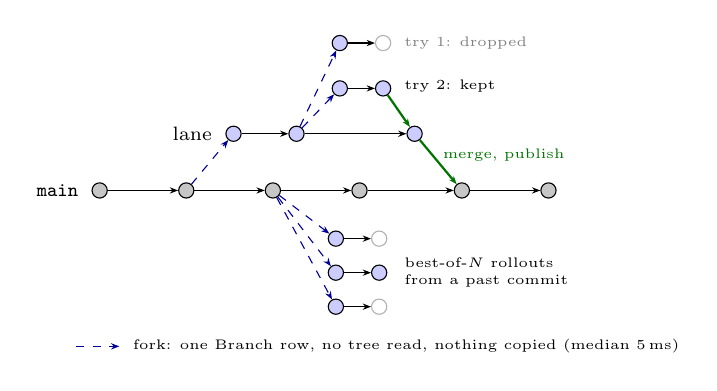
\begin{tikzpicture}[font=\scriptsize,x=1cm,y=0.72cm,
  c/.style={circle,draw,inner sep=0pt,minimum size=5.5pt},
  m/.style={c,fill=gray!45},
  b/.style={c,fill=blue!20},
  d/.style={c,fill=white,draw=gray!60},
  e/.style={-{Stealth[length=3pt]}},
  f/.style={-{Stealth[length=3pt]},dashed,blue!60!black},
  g/.style={-{Stealth[length=3pt]},thick,green!45!black}]
% main
\foreach \i/\x in {0/0,1/1.1,2/2.2,3/3.3,4/4.6,5/5.7}
  \node[m] (m\i) at (\x,0) {};
\foreach \i/\j in {0/1,1/2,2/3,3/4,4/5} \draw[e] (m\i) -- (m\j);
\node[anchor=east] at (-0.15,0) {\texttt{main}};
% lane, forked from main
\node[b] (a1) at (1.7,1) {}; \node[b] (a2) at (2.5,1) {}; \node[b] (a3) at (4.0,1) {};
\draw[f] (m1) -- (a1); \draw[e] (a1) -- (a2); \draw[e] (a2) -- (a3);
\node[anchor=east] at (1.55,1) {lane};
\draw[g] (a3) -- node[right,font=\tiny,pos=0.35]{merge, publish} (m4);
% forks of the fork
\node[b] (t1) at (3.05,2.6) {}; \node[d] (t2) at (3.6,2.6) {};
\node[b] (u1) at (3.05,1.8) {}; \node[b] (u2) at (3.6,1.8) {};
\draw[f] (a2) -- (t1); \draw[e] (t1) -- (t2);
\draw[f] (a2) -- (u1); \draw[e] (u1) -- (u2);
\draw[g] (u2) -- (a3);
\node[anchor=west,font=\tiny,gray] at (3.75,2.6) {try 1: dropped};
\node[anchor=west,font=\tiny] at (3.75,1.85) {try 2: kept};
% best-of-N from a past commit
\foreach \k/\y in {1/-0.85,2/-1.45,3/-2.05} {
  \node[b] (r\k) at (3.0,\y) {};
  \draw[f] (m2) -- (r\k);
}
\node[d] (r1x) at (3.55,-0.85) {}; \draw[e] (r1) -- (r1x);
\node[b] (r2x) at (3.55,-1.45) {}; \draw[e] (r2) -- (r2x);
\node[d] (r3x) at (3.55,-2.05) {}; \draw[e] (r3) -- (r3x);
\node[anchor=west,font=\tiny,align=left] at (3.75,-1.45)
  {best-of-$N$ rollouts\\from a past commit};
% legend
\draw[f] (-0.3,-2.75) -- (0.25,-2.75);
\node[anchor=west,font=\tiny] at (0.3,-2.75)
  {fork: one Branch row, no tree read, nothing copied (median 5\,ms)};
\end{tikzpicture}
\caption{Recursive forks. Any Commit or Layer can start a Branch,
including a past commit and a fork of a fork. A dropped fork costs only the
bytes it changed; a kept one is merged back and published.}
\label{fig:forks}
\end{figure}

\texttt{branch.fork(name, from)} writes one Branch row naming its start: the
newest Layer of \texttt{main}, another Branch's head, or any Commit or Layer
by identifier. It reads no tree and copies no object, so a fork of a fork of
a fork costs the same as the first, and its mount is the same
constant-cost bind (Figure~\ref{fig:forks}). This is what we mean by a
\emph{recursive} filesystem: a fork is a full peer of its parent, and
forking it again costs nothing more. Changes a fork makes are deduplicated against everything
already stored, so a losing fork costs only the bytes it changed. A winning
fork is folded back by \texttt{branch.merge} (a fast-forward when one side
contains the other) and published as \texttt{main}'s next Layer.

\subsection{Many agents, one Branch}
\label{sec:merge}

Agents do not lock files. Each commit merges with the Branch head it finds
when it publishes. Changes to different files land on top. A file changed
on both sides is merged three-way: text is line-merged and overlapping hunks
become a \emph{conflict}; binaries keep the local side. A conflict never
half-lands: nothing is published. In a \ws{}, the merged tree with marker
blocks is installed so the agent can resolve it with ordinary tools, and a
commit is refused while a complete marker block remains.

Some files are rewritten wholesale by tools---lockfiles, build outputs,
caches---and a line merge of them is meaningless. A \texttt{/.lww} file at
the tree root lists gitignore-style patterns; for matching paths changed on
both sides, the newer modification time wins with no conflict, and each
decision is recorded on the commit.

\subsection{Search over filesystem states}
\label{sec:search}

\begin{figure}[t]
\centering
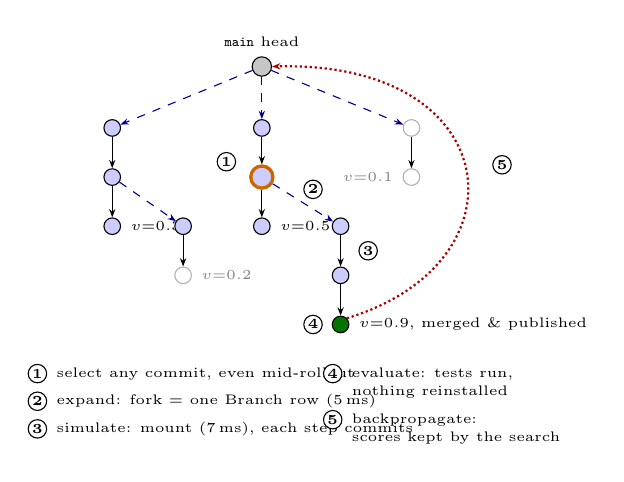
\begin{tikzpicture}[font=\scriptsize,x=1cm,y=0.78cm,
  c/.style={circle,draw,fill=blue!20,inner sep=0pt,minimum size=6pt},
  dr/.style={c,fill=white,draw=gray!60},
  win/.style={c,fill=green!45!black},
  e/.style={-{Stealth[length=3pt]}},
  f/.style={-{Stealth[length=3pt]},dashed,blue!60!black},
  st/.style={circle,draw,fill=white,inner sep=0.6pt,font=\tiny\bfseries},
  sc/.style={font=\tiny,anchor=west}]
% root
\node[c,fill=gray!45,minimum size=7pt] (R) at (2.5,0) {};
\node[anchor=south,font=\tiny] at (R.north) {\texttt{main} head};
% expanded children and their rollouts (every step is a commit)
\node[c] (A)  at (0.6,-1) {}; \node[c] (a1) at (0.6,-1.8) {}; \node[c] (a2) at (0.6,-2.6) {};
\node[c] (B)  at (2.5,-1) {}; \node[c,very thick,draw=orange!80!black,minimum size=8pt] (b1) at (2.5,-1.8) {};
\node[c] (b2) at (2.5,-2.6) {};
\node[dr] (C) at (4.4,-1) {}; \node[dr] (c1) at (4.4,-1.8) {};
\foreach \u/\v in {R/A,R/B,R/C} \draw[f] (\u) -- (\v);
\foreach \u/\v in {A/a1,a1/a2,B/b1,b1/b2,C/c1} \draw[e] (\u) -- (\v);
\node[sc] at (a2.east) {$v{=}0.3$};
\node[sc] at (b2.east) {$v{=}0.5$};
\node[font=\tiny,anchor=east,gray] at (c1.west) {$v{=}0.1$};
% deeper expansions, from mid-rollout commits
\node[c] (e1) at (1.5,-2.6) {}; \node[dr] (e2) at (1.5,-3.4) {};
\draw[f] (a1) -- (e1); \draw[e] (e1) -- (e2);
\node[sc,gray] at (e2.east) {$v{=}0.2$};
\node[c] (d1) at (3.5,-2.6) {}; \node[c] (d2) at (3.5,-3.4) {}; \node[win] (d3) at (3.5,-4.2) {};
\draw[f] (b1) -- (d1); \draw[e] (d1) -- (d2); \draw[e] (d2) -- (d3);
\node[sc] at (d3.east) {$v{=}0.9$, merged \& published};
% backpropagation
\draw[-{Stealth[length=3pt]},densely dotted,thick,red!65!black]
  (d3.north east) .. controls (5.9,-3.2) and (5.6,0.1) .. (R.east);
% step markers
\node[st] at (2.05,-1.55) {1};
\node[st] at (3.15,-2.0)  {2};
\node[st] at (3.85,-3.0)  {3};
\node[st] at (3.15,-4.2)  {4};
\node[st] at (5.55,-1.6)  {5};
% legend
\begin{scope}[shift={(-0.35,-5.0)}]
\node[st] at (0,0) {1}; \node[sc] at (0.12,0) {select any commit, even mid-rollout};
\node[st] at (0,-0.45) {2}; \node[sc] at (0.12,-0.45) {expand: fork = one Branch row (5\,ms)};
\node[st] at (0,-0.9) {3}; \node[sc] at (0.12,-0.9) {simulate: mount (7\,ms), each step commits};
\node[st] at (3.75,0) {4}; \node[sc] at (3.87,0) {evaluate: tests run,};
\node[sc] at (3.87,-0.3) {nothing reinstalled};
\node[st] at (3.75,-0.75) {5}; \node[sc] at (3.87,-0.75) {backpropagate:};
\node[sc] at (3.87,-1.05) {scores kept by the search};
\end{scope}
\end{tikzpicture}
\caption{Monte Carlo tree search over commits. Every node is a Commit---a
complete tree with dependencies and build outputs---and every rollout step
is a node, so search can expand from the middle of an earlier rollout
(orange). Dashed edges are forks, solid edges are steps; dropped Branches
(white) cost only the bytes they changed. Schematic; values are
illustrative.}
\label{fig:mcts}
\end{figure}

Because forks are recursive---one row at any depth---and every step is a
commit,
search algorithms that branch over environment states map directly onto
\sys{}. Figure~\ref{fig:mcts} shows Monte Carlo tree
search~\cite{uct,mctssurvey} over commits. A node is a Commit. Selection
picks any Commit by identifier. Expansion forks it. A simulation mounts a
\ws{} on the new Branch and lets the agent act; each step commits, adding a
median 0.9\,KB for an edit in the nine-agent build. Evaluation runs the
task's tests in the same \ws{} without reinstalling anything, because
ignored files are part of the state. Backpropagation updates statistics
the search keeps outside the tree; \sys{} stores no scores. A dropped
Branch costs only the bytes it changed, and the winner is merged and
published.

Two properties distinguish this from search over sandbox snapshots.
\emph{Every rollout step is a resumable node}: a search can later expand
from the middle of an earlier rollout without replaying it, whereas
container or VM snapshots cost seconds and gigabytes and are taken only at
chosen points. \emph{Expansion cost does not depend on depth}: a fork of a
fork writes one row and mounts in the same constant time as the first.
Siblings that write identical files---the same dependency install, the same
generated output---store them once, because deduplication spans every
Branch on the Store. The same pattern serves best-of-$N$
sampling~\cite{monkeys}, tree-of-thought search~\cite{tot}, reinforcement
learning rollouts whose environment is a source tree, and agents that try a
change to their own code in a fork before adopting it. These are
consequences of the design rather than measured results;
\S\ref{sec:discussion} lists the limits that wide searches would hit.

\subsection{Parallel objects, single-writer metadata}
\label{sec:store}

\begin{figure}[t]
\centering
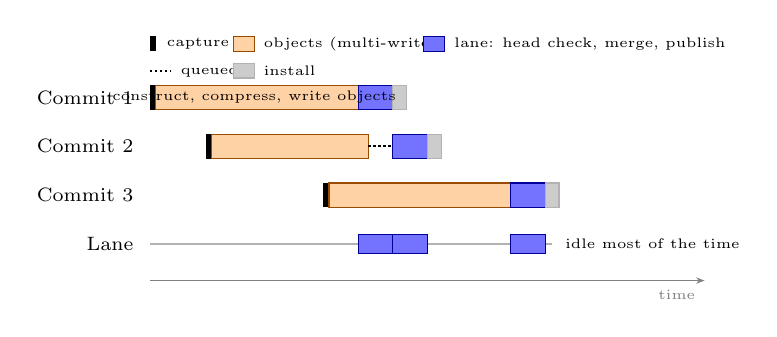
\begin{tikzpicture}[font=\scriptsize,x=0.88cm,y=0.62cm,
  par/.style={fill=orange!35,draw=orange!60!black},
  lane/.style={fill=blue!55,draw=blue!60!black},
  capt/.style={fill=black},
  ins/.style={fill=gray!40,draw=gray!60}]
\newcommand{\row}[7]{%
  \node[anchor=east] at (-0.1,#1) {#2};
  \fill[capt] (#3,#1-0.25) rectangle ++(0.08,0.5);
  \draw[par] (#3+0.08,#1-0.25) rectangle (#4,#1+0.25);
  \draw[densely dotted,thick] (#5,#1) -- (#6,#1);
  \draw[lane] (#6,#1-0.25) rectangle (#7,#1+0.25);
  \draw[ins] (#7,#1-0.25) rectangle ++(0.2,0.5);}
\row{3}{Commit 1}{0.0}{3.0}{3.0}{3.0}{3.5}
\row{2}{Commit 2}{0.8}{3.15}{3.15}{3.5}{4.0}
\row{1}{Commit 3}{2.5}{5.2}{5.2}{5.2}{5.7}
\node[font=\tiny] at (1.5,3) {construct, compress, write objects};
% lane occupancy
\node[anchor=east] at (-0.1,0) {Lane};
\draw[gray!60] (0,0) -- (5.8,0);
\draw[lane] (3.0,-0.2) rectangle (3.5,0.2);
\draw[lane] (3.5,-0.2) rectangle (4.0,0.2);
\draw[lane] (5.2,-0.2) rectangle (5.7,0.2);
\node[font=\tiny,anchor=west] at (5.85,0) {idle most of the time};
\draw[-{Stealth[length=3pt]},gray] (0,-0.75) -- node[below,font=\tiny,pos=0.95]{time} (8,-0.75);
% legend
\begin{scope}[shift={(0,4.1)}]
\fill[capt] (0,-0.15) rectangle ++(0.08,0.3); \node[anchor=west,font=\tiny] at (0.1,0) {capture};
\draw[par] (1.2,-0.15) rectangle ++(0.3,0.3); \node[anchor=west,font=\tiny] at (1.5,0) {objects (multi-writer)};
\draw[lane] (3.95,-0.15) rectangle ++(0.3,0.3); \node[anchor=west,font=\tiny] at (4.25,0) {lane: head check, merge, publish};
\draw[densely dotted,thick] (0,-0.55) -- ++(0.3,0); \node[anchor=west,font=\tiny] at (0.3,-0.55) {queued};
\draw[ins] (1.2,-0.7) rectangle ++(0.3,0.3); \node[anchor=west,font=\tiny] at (1.5,-0.55) {install};
\end{scope}
\end{tikzpicture}
\caption{Three overlapping commits. Object construction runs in parallel,
since immutable, content-addressed objects commute; on SQLite the pack
writes themselves serialize briefly. Only the short metadata step takes the
publication lane; commit~2 queues behind commit~1. Schematic.}
\label{fig:lane}
\end{figure}

The Store separates writes by whether they need an order.
\textbf{Object data is multi-writer.} Objects are immutable and
content-addressed: two writers that store the same object store the same
bytes, so object writes commute and need no global order. Every commit, in
any process, constructs, encodes, compresses and seals its packs on its own,
concurrently with other commits. With PostgreSQL, pack bodies are copied
into the Store before the lane row is locked. With SQLite, each pack batch
is a short write transaction that also takes the Store's directory lock
across processes, so the CPU work---construction, encoding, compression,
sealing---runs in parallel while the batch writes serialize briefly.
\textbf{Metadata is single-writer.} Order matters for the locator index
that makes an object addressable---an identifier is inserted only if
absent, which is unique because one writer inserts---and for history:
Branch heads, Commits and Layers. These go through one writer at a time,
enforced by an in-process FIFO turn and a directory lock across processes
(SQLite) or a lane row (PostgreSQL). A commit holds this \emph{publication
lane} only for its head check, a bounded merge of whatever landed meanwhile,
and the atomic publish; reads never take it (Figure~\ref{fig:lane}).
Writers queue for their turn
instead of failing at once; a writer that cannot get it within a bounded wait
is refused as \texttt{Busy}, and nothing is retried automatically. In the
nine-agent run, 0.66\% of writes were refused this way
(\S\ref{sec:eval-casestudy}).

This is the split used by lakehouse table formats, which write data files
in parallel and serialize commits to a metadata log~\cite{deltalake}, and by
Git, which writes objects freely and updates references atomically. We chose
it over sharding or a multi-writer metadata engine because agents' tool
calls are separated by model latency, so concurrent publications on one
Store are uncommon: the uncontended commit is the case to optimize, and
contention must only stay correct and bounded. Work that grows with tree
size, history length or Branch count inside the lane is treated as a
defect.

The SQLite Store runs in WAL mode with \texttt{synchronous=OFF}. It survives
process failure but not a kernel or VM crash, a deliberate trade for
latency that we discuss in \S\ref{sec:durable}.

\section{Recording Everything: Share First, Then Compress}
\label{sec:storage}

Every commit names a whole tree, dependencies and build outputs included,
so recording everything is practical only if what did not change costs
nothing. \sys{} stores committed state as a Merkle DAG of immutable,
content-addressed objects. It \emph{shares first}: unchanged subtrees,
files and chunks keep their identities and are reused, across steps,
Branches and projects. It \emph{compresses second}: what is genuinely new
is delta-encoded against one well-chosen base and compressed, inside the
commit that creates it. Section~\ref{sec:eval-granularity} shows which of
the two dominates depends on how often agents commit, and
Appendix~\ref{app:pipeline} traces the pipeline through 14 workload
patterns and two worked examples; Appendix~\ref{app:analysis} bounds the
time and storage each change costs and how storage grows over many
snapshots.

\subsection{Objects and identity}

Each object is a role-tagged value in a fixed envelope. Its identifier is
the BLAKE3 hash~\cite{blake3} of a domain string,
\texttt{layerfs/object/v2\textbackslash 0}, followed by the canonical
bytes. Thirteen roles form the tree: a
filesystem root names a B$^+$-tree inode table keyed by a stable serial; an
inode value names a content root and metadata; content is a whole-file
object, a file state over a B$^+$-tree of extent pages referencing chunks,
a directory B$^+$-tree from names to serials, or a symlink. Decoders accept
exactly one encoding per value, and references are derived from bytes,
never supplied by callers.

Physical representation---compression, delta base, pack location---is
outside the identifier. Every read rebuilds canonical bytes and re-hashes
them, so a corrupted or mis-decoded record is detected at read time.

\subsection{Structural sharing and exact reuse}
\label{sec:reuse}

\begin{figure}[t]
\centering
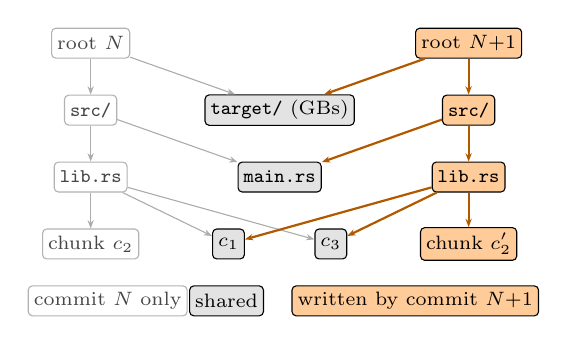
\begin{tikzpicture}[font=\scriptsize,x=1cm,y=0.85cm,
  n/.style={draw,rounded corners=1.5pt,inner sep=2pt,minimum height=0.38cm},
  old/.style={n,fill=white,draw=gray!60,text=gray!55!black},
  shared/.style={n,fill=gray!22},
  new/.style={n,fill=orange!40},
  e/.style={-{Stealth[length=3pt]},gray!65},
  ne/.style={-{Stealth[length=3pt]},orange!70!black,thick}]
\node[old]    (R)   at (0.8,3) {root $N$};
\node[new]    (R2)  at (5.6,3) {root $N{+}1$};
\node[old]    (B)   at (0.8,2) {\texttt{src/}};
\node[shared] (A)   at (3.2,2) {\texttt{target/} (GBs)};
\node[new]    (B2)  at (5.6,2) {\texttt{src/}};
\node[old]    (F3)  at (0.8,1) {\texttt{lib.rs}};
\node[shared] (F4)  at (3.2,1) {\texttt{main.rs}};
\node[new]    (F32) at (5.6,1) {\texttt{lib.rs}};
\node[old]    (C2)  at (0.8,0) {chunk $c_2$};
\node[shared] (C1)  at (2.55,0) {$c_1$};
\node[shared] (C3)  at (3.85,0) {$c_3$};
\node[new]    (C22) at (5.6,0) {chunk $c_2'$};
\draw[e] (R) -- (B);  \draw[e] (R) -- (A);
\draw[e] (B) -- (F3); \draw[e] (B) -- (F4);
\draw[e] (F3) -- (C2); \draw[e] (F3) -- (C1); \draw[e] (F3) -- (C3);
\draw[ne] (R2) -- (A); \draw[ne] (R2) -- (B2);
\draw[ne] (B2) -- (F4); \draw[ne] (B2) -- (F32);
\draw[ne] (F32) -- (C1); \draw[ne] (F32) -- (C22); \draw[ne] (F32) -- (C3);
\node[old,anchor=west]    (L1) at (0.0,-0.85) {commit $N$ only};
\node[shared,anchor=west] (L2) at (2.05,-0.85) {shared};
\node[new,anchor=west]    (L3) at (3.35,-0.85) {written by commit $N{+}1$};
\end{tikzpicture}
\caption{Structural sharing after a one-line edit to \texttt{lib.rs}.
Commit $N{+}1$ writes only the path from the changed chunk to the root;
every other object, including all of \texttt{target/}, is referenced, not
copied. Simplified: directories, the inode table and large files are
B$^+$-trees, so the new path is a few pages.}
\label{fig:sharing}
\end{figure}

A commit rebuilds only the paths from changed entries to the root.
Unchanged directories keep their stored roots, an inode-table page that no
change reaches is not rewritten, and an unchanged file keeps its content
root, so committing a 9\,GB tree after a one-line edit writes a few pages
(Figure~\ref{fig:sharing}).
Publishing \texttt{main}'s next Layer names an existing root rather than
copying it.


Objects reach storage in batches (\emph{waves}). Duplicates within a wave
are compared byte for byte. An object already stored with the same
identifier, role and length is reused without reading it back; integrity is
deferred to the read path, which authenticates every decoded object.
Concurrent writers are arbitrated by insert-if-absent locators, and a losing
writer compares its bytes with the winner's. Reuse spans the whole Store:
across steps, Branches and projects.

\subsection{Chunking and localized edits}
\label{sec:edits}

Files below a per-Store cutoff (128\,KiB by default) are single whole-file
objects. Larger files are split by a FastCDC-style~\cite{fastcdc} GEAR
scanner with an 8\,KiB minimum, 16\,KiB normalization point and 32\,KiB
maximum. The chunking profile is hashed into every file state so the
partition cannot drift silently. Runs of zeros exploit the scanner's
32\,KiB period: interior zero chunks become a repeat count and identical
mapping pages are reused, so construction work grows with tree height rather
than hole length.

A \emph{localized edit} splits stored extents at its boundaries, discards
the replaced middle unread, chunks only the replacement bytes and rebuilds
pages only on the join paths. Unchanged extents keep their identities,
including slices of stored chunks, so the same overwrite reads 3 pages on an
8\,MB file and 4 on a 24\,MB file. The price is that equal bytes can have
different roots depending on edit history; diff and merge therefore compare
bytes (skipping shared extents) rather than roots.

\subsection{Delta bases from filesystem events}
\label{sec:delta}

Each new payload object (whole file or chunk) first receives an independent
record: zstd~\cite{zstd} level~3, or raw when a 1\,KiB probe predicts no
gain. Selection then makes \emph{at most one} delta trial: a zstd frame
compressed with a single base payload as prefix. The delta is kept only if
its full record, including the 32-byte base identifier, is strictly smaller.

The single base is chosen from \emph{filesystem events} rather than content
search:
\begin{itemize}
\item \textbf{Localized edits.} An aligner walks the old extent map and
  offers each new chunk the old chunk it overlaps most.
\item \textbf{Rename-over.} Git, editors and package managers save by
  writing a temporary file and renaming it over the original, producing a
  new inode that an edit-based scheme never connects to the old file. The
  \ws{} overlay records the replaced file when \texttt{rename()} runs and
  offers it as the base.
\item \textbf{Recreate at a path.} A file deleted and recreated at the same
  path is offered the file the base held there.
\item \textbf{Similarity fallback.} Whole files with no event-derived base
  consult a bounded, persisted resemblance index of eight-hash bottom-$k$
  signatures (8,192 entries, 704\,KiB in total), in the spirit of
  super-features~\cite{shilane,finesse}.
\end{itemize}
Rename-over tracking reduced bytes stored for a replayed agent's Git index
churn by 80\% (1,463,988 to 297,095 bytes), and small-file base selection on
rename-over and recreate cut payload by 44\% on a new-path-per-version
workload (\S\ref{sec:eval-mech}).

\subsection{Bounded chains}

Deltas create read dependencies. Chains are bounded by depth (16 for whole
files, 8 for chunks and metadata) and by work: a payload chain's decoded
bytes must stay within 4\X{} the cutoff and its encoded bytes within
2\X{}. When a candidate's chain reaches a limit, the dependent re-bases
onto the chain's independent root rather than being stored in full. A base
whose delta trials keep losing---for example the old last chunk offered to
every appended chunk---is backed off after eight losses. There is no
background repacking or garbage collection: a representation chosen at
commit time is permanent, and the selection must therefore be cheap and
bounded.

\subsection{Metadata}

Per-commit cost on small edits is dominated by metadata, not payload. Inode
values are pooled, with leaves storing (serial, ordinal) pairs; values live
in immutable, field-packed, checksummed blocks of at most 4,000 bytes. Inode
table branches, directory pages and extent pages may be stored as
COPY/INSERT programs against the page they replace, under the metadata depth
cap.

\subsection{Packs}

New records are grouped by lane (tree pages, chunks, compact whole files,
singletons), sealed into append-only packs of at most 256\,KiB, and stored as
database rows; triggers forbid updating or deleting a sealed pack. A locator
row maps each identifier to its pack, group and record.

\section{Implementation and Performance Engineering}
\label{sec:impl}

\sys{} is written in Rust, with a Node.js SDK and a command-line client.
On Linux it serves \ws{}s through FUSE using \texttt{fuser} 0.18 with three
small patches (signed timestamps, explicit session lifecycle, and receive
buffers sized to \texttt{max\_write} rather than 16\,MiB); on macOS it serves
a loopback NFSv3 export. It negotiates 128\,KiB reads and writes and keeps
kernel write-back off. We optimized by instrumenting exact counters (SQL
statements, Store round trips, overlay jobs, delta trials) and removing
work, keeping one construction producer per commit.

\paragraph{Isolating \ws{}s.} The first daemon served all \ws{}s through one
overlay database owned by a single thread with class queues and admission
credits; it saturated near 7,000 file operations per second. Giving each
\ws{} its own overlay file and a single short-hold lock cut statements by
12--61\% across our case set and a four-\ws{} commit from 67.4\,s to 13.4\,s
(one sample; one dense-rewrite case regressed by 45\%).

\paragraph{Flat commits on long histories.} Commit cost first grew with
Branch length, because each commit re-read every inode leaf under an edited
branch page. Storing inode values as Store rows and reading only children a
change reaches reduced pack reads per commit from 2,198 to 15 at 2,000 prior
commits; mounted commit latency stayed at a 13--16\,ms median from 0 to 950
earlier commits.

\paragraph{Reads never wait for writes.} Removing an accidental dependency
of reads on the publication lane cut p95 read latency in a multi-agent
replay from 96\,ms to 10\,ms.

\paragraph{Large new data.} Appending 500\,MiB once took 6.9\,s to commit.
Seven fixes---a producer thread feeding the Save through a
bounded queue, backing off losing delta bases (26,966 trials to 22), batched
locator lookups (53,500 calls to 144), hashing each pack once, reading
overlay rows in whole windows, moving WAL checkpoints off the commit path,
and reclaiming after the reply---brought it to 1.40\,s. An eighth trades 1\%
more storage for 37\% faster log-append commits; we report both.

\paragraph{Import and exec.} A 500\,MiB import from macOS into the Linux
worker fell from 32.1\,s to 5.0\,s after replacing base64 frame encoding
with binary attachments and pipelining parts. Restoring file timestamps when
unpacking Sandbox images stopped Python from recompiling every import,
cutting a typical edit step from about 105\,ms to 62\,ms.

\section{Evaluation}
\label{sec:eval}

We start with a 13-hour build by nine agents that used \sys{} as their
only filesystem, then ask: (1) how much does recording everything cost
compared with agent and snapshot filesystems; (2) which storage mechanism
does the work, and when; (3) how fast is the per-call lifecycle; (4) where
is \sys{} slower; and (5) is it correct.

\subsection{Setup and methodology}

All measurements ran on an Apple M3 Max (14 cores, 36\,GiB) under macOS,
with \sys{} and baselines inside Docker Desktop's Linux VM (8 vCPUs,
7.75--8\,GiB), using SQLite Stores, one construction worker, and binaries,
bundles and images pinned by hash. The host was shared with other workloads
(1-minute load 4--29). Storage figures are exact byte counts. Most timings
are single samples and we treat them as diagnostics; the ovnfs comparison
uses three samples per case and reports medians, with a verified cold
boundary before every commit and read: each system's files are flushed and
evicted with \texttt{posix\_fadvise(DONTNEED)}, and a boundary counts only
when \texttt{fincore} reports zero resident bytes (1,014 of 1,014 did).
Daemon caches, VM metadata caches and the host cache beneath the VM disk
were not controlled. Every Branch head was verified against an oracle.
\dnote{Before submission: rerun on dedicated native Linux, same route into
every system, $N\geq5$ samples with intervals.}

\paragraph{Driving \sys{}.} Every harness drives \sys{} only through the
public command line (Appendix~\ref{app:cli}), in the sequence below; times
in \S\ref{sec:eval} include each command's process launch and routing.

{\footnotesize
\begin{verbatim}
# once per case
layerfs store create s     # or: store connect s <url>
layerfs machine start m    # docker or a VM
layerfs store push s m     # Store next to the Sandboxes
layerfs project init s/p <folder>
layerfs sandbox create s/p box m
# once per shell call
layerfs workspace mount box <branch>
layerfs workspace exec <ws> '<command>'
layerfs workspace commit <ws>
layerfs workspace unmount <ws>
# measurement and teardown
layerfs store stats s; layerfs project stats s/p
layerfs sandbox close box; layerfs store remove s
\end{verbatim}
}

\paragraph{Baselines.} ovnfs~\cite{ovnfs} (commit \texttt{5d54cb0}), which
packs, compresses and delta-encodes its store, run on ext4 (no reflinks).
Btrfs with zstd, with and without offline deduplication (bees), from an
earlier unpaired run. Git packs as an offline storage reference: Git is not
a live filesystem and its commit scans the tree, so we compare only its
packed size.

\paragraph{Workloads.} (i) \emph{History shapes}: a real 65.0\,MB,
9,404-file repository with a seeded edit model (70\% line edits, 10\% new
files, 5\% deletes, 10\% renames, 5\% appends; five operations per commit)
on one or several Branches. (ii) \emph{Large files}: 100\,B overwrites,
inserts and 16\,KiB appends on 5--500\,MiB incompressible files, and
500\,MiB create, append, remove and truncate. (iii) \emph{Real history}:
157 snapshots of a public agent-harness repository (every 100th of 15,632
commits), replayed by rewriting each changed file whole. (iv)
\emph{Single-mechanism micro cases}. (v) \emph{Multi-agent runs} of an
open-source coding harness on \sys{}: a 13-hour, nine-agent build on a 2.0
release build (\S\ref{sec:eval-casestudy}) and two earlier runs on 1.x.

\subsection{A 13-hour, nine-agent build}
\label{sec:eval-casestudy}

\begin{table}[t]
\centering
\small
\setlength{\tabcolsep}{3pt}
\begin{tabular}{l r r r r}
\toprule
\multicolumn{5}{l}{\textbf{Run}: 9 agents, 13\,h 22\,min, 4,354 commits, 211 Branches} \\
\midrule
Commit kind & Commits & New & Stored & Total \\
 & & (median) & (median) & stored \\
\midrule
File edits      & 3,051 & 29\,KB  & \textbf{0.9\,KB} & 0.07\,GB \\
Builds, tests   & 1,195 & 9.8\,MB & 1.3\,MB & 4.68\,GB \\
Merges          & 67    & 188\,KB & 16\,KB  & 0.002\,GB \\
\bottomrule
\end{tabular}
\caption{Storage of the nine-agent build by commit kind (totals in
Figure~\ref{fig:quarrybytes}). Every commit records the whole project tree,
about 9\,GB including build folders. \sys{} at
\texttt{c5e58735bb}, release build, SQLite Store.}
\label{tab:quarry}
\end{table}

\begin{figure}[t]
\centering
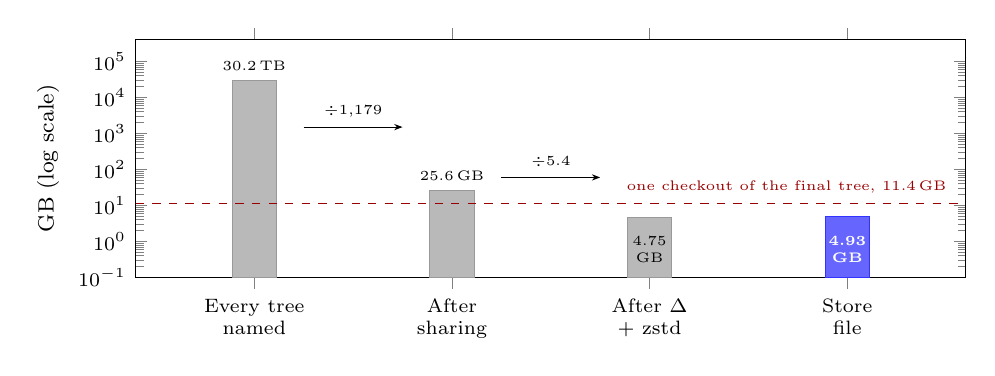
\begin{tikzpicture}
\begin{axis}[
  ybar, bar width=16pt, width=\columnwidth, height=4.6cm,
  ymode=log, log origin=infty, ymin=0.1, ymax=4e5,
  ylabel={GB (log scale)}, ylabel style={font=\footnotesize},
  xtick={0,1,2,3}, xmin=-0.6, xmax=3.6,
  xticklabels={Every tree\\named, After\\sharing, After $\Delta$\\+ zstd, Store\\file},
  xticklabel style={font=\scriptsize,align=center},
  yticklabel style={font=\scriptsize},
  ytick={0.1,1,10,100,1000,10000,100000},
  clip=false]
\addplot+[fill=gray!55,draw=gray!80,mark=none,bar shift=0pt] coordinates {(0,30200) (1,25.6) (2,4.75)};
\addplot+[fill=blue!60,draw=blue!80,mark=none,bar shift=0pt] coordinates {(3,4.93)};
\draw[dashed,red!60!black] (axis cs:-0.6,11.4) -- (axis cs:3.6,11.4);
\node[font=\tiny,red!60!black,anchor=south east] at (axis cs:3.55,11.4) {one checkout of the final tree, 11.4\,GB};
\node[font=\tiny,anchor=south] at (axis cs:0,30200) {30.2\,TB};
\node[font=\tiny,anchor=south] at (axis cs:1,25.6) {25.6\,GB};
\node[font=\tiny,align=center] at (axis cs:2,0.6) {4.75\\GB};
\node[font=\tiny,align=center,white] at (axis cs:3,0.6) {\textbf{4.93}\\\textbf{GB}};
\draw[-{Stealth[length=3pt]}] (axis cs:0.25,1500) -- node[above,font=\tiny]{$\div$1,179} (axis cs:0.75,1500);
\draw[-{Stealth[length=3pt]}] (axis cs:1.25,60) -- node[above,font=\tiny]{$\div$5.4} (axis cs:1.75,60);
\end{axis}
\end{tikzpicture}
\caption{Where the nine-agent build's bytes went. 4,354 commits name
30.2\,TB of whole trees; sharing removes all but 25.6\,GB, deltas and
compression leave 4.75\,GB, and the Store file is smaller than one checkout
of the final tree.}
\label{fig:quarrybytes}
\end{figure}

\begin{table}[t]
\centering
\small
\begin{tabular}{l r r r}
\toprule
Call & Median & p90 & Calls \\
\midrule
\texttt{workspace.mount}   & 7\,ms   & 16\,ms  & 1,121 \\
\texttt{workspace.unmount} & 14\,ms  & 35\,ms  & 1,121 \\
\texttt{workspace.commit}  & 204\,ms & 1.06\,s & 1,186 \\
\texttt{file.read}         & 6\,ms   & 10\,ms  & 4,926 \\
\texttt{file.edit}         & 14\,ms  & 25\,ms  & 982 \\
\texttt{branch.fork}       & 5\,ms   & 8\,ms   & 93 \\
\texttt{branch.merge}      & 263\,ms & 479\,ms & 67 \\
\texttt{branch.publish} (11\,GB tree) & 7\,ms & 11\,ms & 39 \\
\bottomrule
\end{tabular}
\caption{\sys{} call latency in the nine-agent build, after the release
build was installed mid-run.}
\label{tab:quarry-lat}
\end{table}

Nine agents---a lead and eight workers in four lanes---built a
SQLite-compatible database engine in Rust through an open-source agent
harness, with \sys{} as their only filesystem. Every shell call ran in a
\ws{} (mount, run, commit, unmount); each lane worked on its own Branch, and
the lead merged lanes on an integration Branch and published to
\texttt{main}. The run ended when a terminal check passed on a fresh fork of
\texttt{main}: 15 crates and about 87,000 lines of Rust, 1,567 passing tests,
and 16 of 16 acceptance checks against the reference \texttt{sqlite3}.

\paragraph{Storage.} Every commit recorded the whole tree, about 9\,GB
including \texttt{target/}. The 4,354 commits on 211 Branches name 30.2\,TB
of trees, which reduce to 25.6\,GB of distinct content and then to 4.75\,GB
after deltas and compression. The Store file is 4.93\,GB, less than half of
one checkout of the final tree (Figure~\ref{fig:quarrybytes}). Edits are
nearly
free: the 3,051 file-edit commits stored a median 0.9\,KB each, although
every one recorded a 9\,GB tree. Builds produced 98.5\% of the stored
bytes. Keeping ignored files and build outputs therefore costs what the
agents \emph{produce}, not what the tree \emph{holds}.

\paragraph{Latency.} Table~\ref{tab:quarry-lat} shows \sys{} calls over the
run. Borrowing a \ws{} cost a median 7\,ms to mount and 14\,ms to unmount
across 1,121 shell calls. Forks took 5\,ms, and publishing an 11\,GB tree to
\texttt{main} took 7\,ms because a Layer names an existing root. Commits
took a median 204\,ms because many carried fresh build outputs.

\paragraph{State outlives compute.} Midway through the run, a settings save
in the host application reloaded the harness plugin and ended the live run.
No work was lost: every agent's state was in its Branches, and the run
resumed from them.

\paragraph{What went wrong.} Of 59,331 \sys{} calls, 1.2\% were refused,
and 35 of 5,312 writes (0.66\%) were refused because the Store was busy.
Concurrent writes to the Store were sometimes refused with an operating
system \texttt{NotFound} error, which agents worked around by retrying.
Stopping an agent's turn left its command running in the Sandbox while
\ws{} status reported it idle. Copying a warm \texttt{target/} with a file
call took about a minute. Two \sys{} changes were installed while the agents
kept working: a release build replacing a debug build of the Linux bundle,
and a fix that stopped unmount from waiting for a commit's deferred cleanup;
the latencies above are from after both. The harness's operator checked the
run every 10--15 minutes and steered it when it stalled.

\begin{table*}[t]
\centering
\small
\begin{tabular}{l l r r r r r r}
\toprule
& & \multicolumn{2}{c}{Stored at end (MB)} & \multicolumn{2}{c}{Added per commit} &
\multicolumn{2}{c}{Commit, cold (ms)} \\
\cmidrule(lr){3-4}\cmidrule(lr){5-6}\cmidrule(lr){7-8}
Case & Shape & ovnfs & \sys{} & ovnfs & \sys{} & ovnfs & \sys{} \\
\midrule
S1 & 1 Branch $\times$ 40 commits        & 26.37 & \textbf{23.97} & 32.2\,KB & \textbf{5.1\,KB} & 83.8 & \textbf{41.9} \\
S2 & 5 Branches $\times$ 3 commits       & 26.09 & \textbf{23.88} & 66.6\,KB & \textbf{5.5\,KB} & 77.5 & \textbf{35.8} \\
S3 & fork chain 4 deep $\times$ 3        & 25.59 & \textbf{23.81} & 41.6\,KB & \textbf{6.5\,KB} & 73.7 & \textbf{39.1} \\
S4 & 5 Branches, same commit             & 25.62 & \textbf{23.78} & 105.7\,KB & \textbf{4.9\,KB} & 70.6 & \textbf{46.0} \\
\midrule
L100 & 100\,MiB, 100\,B overwrite $\times$10 & 1,154.7 & \textbf{106.3} & 104.9\,MB & \textbf{5.3\,KB} & 221.1 & \textbf{24.5} \\
L10  & 10\,MiB, 100\,B overwrite $\times$20  & 221.5 & \textbf{10.9} & 10.5\,MB & \textbf{5.5\,KB} & 190.9 & \textbf{24.4} \\
I10  & 10\,MiB, 100\,B insert $\times$10     & 116.6 & \textbf{10.9} & 10.5\,MB & \textbf{5.3\,KB} & 197.9 & \textbf{25.5} \\
A5   & 5\,MiB, 16\,KiB append $\times$20     & 18.7 & \textbf{5.9} & 613\,KB & \textbf{18.4\,KB} & 145.2 & \textbf{19.5} \\
L500 & 500\,MiB, 100\,B overwrite $\times$5  & 3,146.9 & \textbf{530.4} & 524.3\,MB & \textbf{7.4\,KB} & 603.9 & \textbf{28.1} \\
\bottomrule
\end{tabular}
\caption{\sys{} versus ovnfs on code-edit histories (S1--S4, from a 65\,MB,
9,404-file tree) and large-file edits. Medians of three samples; commit
times are measured after a verified cold boundary and include each system's
route (CLI-to-worker for \sys{}, \texttt{docker exec} for ovnfs). \sys{} at
\texttt{b9c4adcb}; ovnfs at \texttt{5d54cb0}.}
\label{tab:ovnfs}
\end{table*}

\subsection{Storage against agent filesystems}
\label{sec:eval-storage}

Table~\ref{tab:ovnfs} compares \sys{} with ovnfs. On code-edit histories
the imported base tree dominates the total, and ovnfs ends 7.6--10\% larger.
The per-commit cost differs far more: ovnfs adds 32--106\,KB per commit and
\sys{} 4.9--6.5\,KB, a 6--22\X{} gap. About two thirds of \sys{}'s
per-commit bytes are metadata. On large files the gap is structural: ovnfs
stores each overwritten or inserted-into version in full (about 100\% of raw
bytes), while \sys{} stores the original plus 5--7\,KB per commit (5--17\%
of raw); the 100\,B overwrite itself costs 153\,B of payload at every file
size, and the rest is metadata (Figure~\ref{fig:comparison} contrasts
whole-file copy-up, block copy-on-write and \sys{} for this edit). Appends are the one large-file case where ovnfs compresses well
(16\% of raw); \sys{} stores the incompressible appended bytes nearly as is
and ends at 5\%.

\begin{figure}[t]
\centering
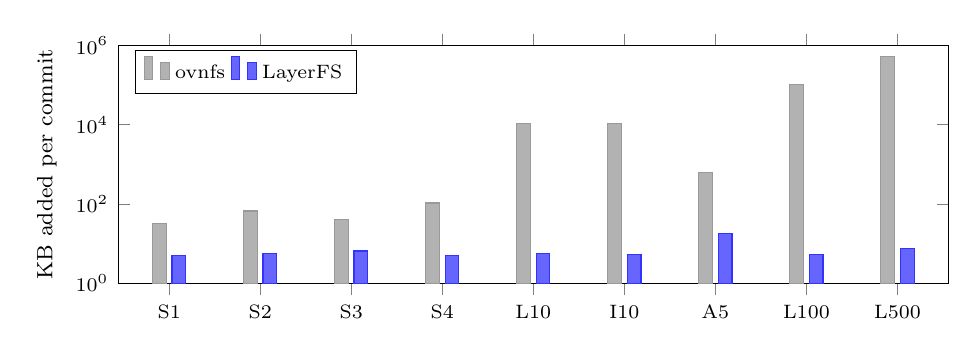
\begin{tikzpicture}
\begin{axis}[
  ybar, bar width=5pt, width=\columnwidth, height=4.6cm,
  ymode=log, log origin=infty, ymin=1, ymax=1e6,
  ylabel={KB added per commit}, ylabel style={font=\footnotesize},
  symbolic x coords={S1,S2,S3,S4,L10,I10,A5,L100,L500},
  xtick=data, ticklabel style={font=\scriptsize},
  legend style={font=\scriptsize,at={(0.02,0.98)},anchor=north west,legend columns=2},
  enlarge x limits=0.07]
\addplot+[fill=gray!60,draw=gray!80] coordinates
  {(S1,32.2) (S2,66.6) (S3,41.6) (S4,105.7) (L10,10500) (I10,10500) (A5,613) (L100,104900) (L500,524300)};
\addplot+[fill=blue!60,draw=blue!80] coordinates
  {(S1,5.1) (S2,5.5) (S3,6.5) (S4,4.9) (L10,5.5) (I10,5.3) (A5,18.4) (L100,5.3) (L500,7.4)};
\legend{ovnfs, \sys{}}
\end{axis}
\end{tikzpicture}
\caption{Bytes added per commit (log scale), from Table~\ref{tab:ovnfs}.}
\label{fig:percommit}
\end{figure}

\subsection{Recording everything on real histories}
\label{sec:eval-history}

\paragraph{157 snapshots of a real repository.} Replaying 157 snapshots of a
public agent-harness repository (4.94\,GB of trees; 75,929 distinct files
totalling 892\,MB; two thirds of distinct files under 8\,KiB), \sys{} keeps
every snapshot as a mountable commit in 100.1\,MB, 49\X{} less than the
trees. Btrfs with zstd snapshots required 1,994.6\,MB (19.9\X{}), and adding
the bees deduplicator raised it to 2,068.9\,MB including its state, because
sharing metadata grew by more than the data it merged. A Git pack of the
same states is 55.1\,MB, smaller than \sys{}. The replay rewrites each
changed file whole, which removes Btrfs's in-place extent sharing by
construction, and the Btrfs run was not paired with this \sys{} build; we
rerun it in the final evaluation. \dnote{Release-labelled v1.0.0 run at
\texttt{e5c7aaae05}; rerun on 2.0.}

\begin{table}[t]
\centering
\small
\setlength{\tabcolsep}{2pt}
\begin{tabular}{l r r r r r}
\toprule
Case & Raw & Stored & Raw/ & Dedup & $\Delta$+zstd \\
 & MB & MB & stored & & \\
\midrule
D10 17 states & 561 & 47.9 & 11.7\X & 1.48\X & 9.26\X \\
D03 53 states & 1,677 & 61.0 & 27.5\X & 2.84\X & 11.6\X \\
H01 500 commits & 32,477 & 26.5 & 1,226\X & -- & -- \\
H03 50 same Br. & 3,316 & 23.8 & 139\X & -- & -- \\
H05 20 proj./1 Store & 7,802 & 28.3 & 276\X & -- & -- \\
H06 20 proj./20 Stores & 7,802 & 471.4 & 16.6\X & -- & -- \\
\bottomrule
\end{tabular}
\caption{Reduction on real and seeded histories (SQLite, \texttt{7691ac20}).
\emph{Dedup} is raw over new canonical bytes; \emph{delta+zstd} is new
canonical over new stored bytes. H rows start from a 65\,MB imported base.}
\label{tab:history}
\end{table}

\paragraph{History shapes.} Table~\ref{tab:history} breaks down the
reduction. On the real history at two sampling strides (D10, D03), exact
deduplication contributes 1.5--2.8\X{} and delta encoding plus compression
9.3--11.6\X; Store overhead (database pages, indexes and free space around
the packs) adds 17--20\%. Against the offline Git reference, \sys{} is
1.15--1.27\X{} larger. On seeded histories over a 65\,MB base, 500 commits
add about 5.9\,KB each (2,990\,B of new packs, two thirds metadata); fifty
identical Branches add about 270\,KB in total; and twenty projects sharing
one Store need 16.7\X{} less space than twenty separate Stores.

\paragraph{Earlier multi-agent runs.} Two earlier runs of the same harness,
on a 1.x build, used \sys{} as the agents' only filesystem. Building a
trip-planning web application (1 lead and 7 worker agents, 56 minutes)
produced 147 commits on 31 Branches, whose snapshots total 91.5\,MB, in a
1.21\,MB Store. Building a SQL database in Rust with every build's
\texttt{target/} directory committed (8 agents, 4 hours 16 minutes)
produced 913 commits on 56 Branches whose snapshots total 4.93\,TB, in an
8.90\,GB Store---less than one copy of the final tree (13.5\,GB).
\dnote{Site-reported v1 runs; cite the run record.}

\subsection{Commit granularity decides what saves space}
\label{sec:eval-granularity}

\begin{figure}[t]
\centering
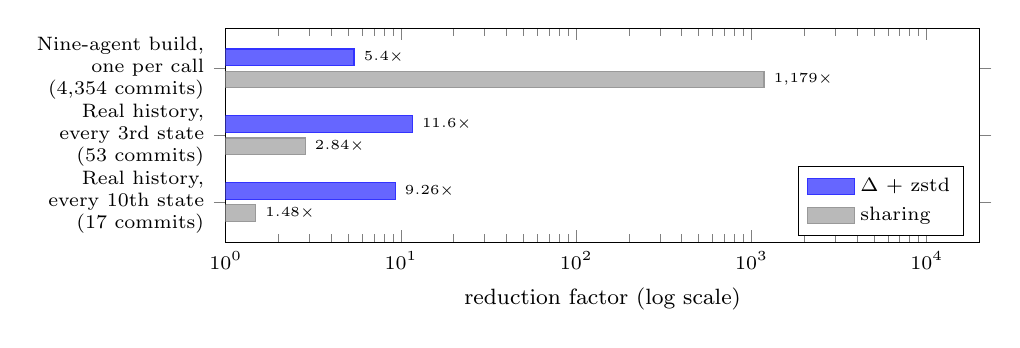
\begin{tikzpicture}
\begin{axis}[
  xbar, bar width=6pt, width=0.92\columnwidth, height=4.3cm,
  xmode=log, log origin=infty, xmin=1, xmax=2e4,
  xlabel={reduction factor (log scale)}, xlabel style={font=\footnotesize},
  ytick={0,1,2}, ymin=-0.6, ymax=2.6,
  yticklabels={{Real history,\\every 10th state\\(17 commits)},
               {Real history,\\every 3rd state\\(53 commits)},
               {Nine-agent build,\\one per call\\(4,354 commits)}},
  yticklabel style={font=\scriptsize,align=right},
  xticklabel style={font=\scriptsize},
  legend style={font=\scriptsize,at={(0.98,0.03)},anchor=south east},
  legend cell align=left,
  point meta=rawx,
  nodes near coords={\pgfmathprintnumber[fixed,precision=2]{\pgfplotspointmeta}\X},
  nodes near coords style={font=\tiny,black,anchor=west},
  nodes near coords align={horizontal},
  area legend, reverse legend,
  enlarge y limits=0]
\addplot+[fill=gray!55,draw=gray!80,mark=none] coordinates {(1.48,0) (2.84,1) (1179,2)};
\addplot+[fill=blue!60,draw=blue!80,mark=none] coordinates {(9.26,0) (11.6,1) (5.4,2)};
\legend{sharing, $\Delta$ + zstd}
\end{axis}
\end{tikzpicture}
\caption{Which mechanism does the work. \emph{Sharing} is logical bytes
over distinct canonical bytes; \emph{delta + zstd} is distinct canonical
bytes over stored bytes. Per-call commits make sharing dominant; coarse snapshots
shift the load to deltas.}
\label{fig:granularity}
\end{figure}

Figure~\ref{fig:granularity} splits the reduction into the two stages of
\S\ref{sec:storage}. When agents commit after every tool call, consecutive
states differ in a few files, so nearly every object in the next commit
already exists: sharing reduces 30.2\,TB of trees to 25.6\,GB, a 1,179\X{}
reduction, and deltas plus compression contribute a further 5.4\X{}, mostly
on fresh build outputs. When the same kind of source tree is snapshotted
coarsely---every 3rd or 10th of 157 historical states, with each changed
file rewritten whole---many files change between snapshots, each a new
version close to an old one. Sharing then contributes only 1.5--2.8\X{} and
delta encoding carries the load (9.3--11.6\X). The per-call model that makes
\ws{}s ephemeral is also what makes sharing so effective; delta encoding
matters for rewritten files, build outputs and coarse imports. The two
workloads differ in more than granularity---the build includes compiled
outputs, the replay does not---so we read the figure as indicative.
\dnote{Control for content: replay the nine-agent run's states at strides
1, 3 and 10.}

\subsection{Mechanism contributions}
\label{sec:eval-mech}

\begin{table}[t]
\centering
\small
\setlength{\tabcolsep}{3pt}
\begin{tabular}{l r r r}
\toprule
Micro case & Raw/stored & Dedup & Delta+zstd \\
\midrule
M01 10,000 tiny files        & 0.91\X & 0.94\X & 1.05\X \\
M02 tree + 10 copies         & 16.97\X & 11.90\X & 1.45\X \\
M03 1\% in-place edits       & 29.27\X & 1.00\X & 32.12\X \\
M04 same, rename-over        & 28.02\X & 1.00\X & 32.04\X \\
M05 same, new path           & 25.15\X & 1.00\X & 30.07\X \\
M06 64\,MiB random + 5 edits & 5.87\X & 5.90\X & 1.00\X \\
M07 random / zeros / text    & 4.29\X & 2.99\X & 1.45\X \\
M08 SQLite DB, 1\% churn     & 13.73\X & 3.21\X & 4.44\X \\
\bottomrule
\end{tabular}
\caption{Single-mechanism cases (SQLite Store, \texttt{7691ac20}).}
\label{tab:micro}
\end{table}

Table~\ref{tab:micro} isolates mechanisms. Copies (M02) are absorbed by
exact reuse; small edits to text files (M03) by deltas, whether the editor
writes in place, renames over the original (M04) or writes a new path (M05,
which falls back to the similarity index); edits to a large random file
(M06) by chunk reuse, with each edit adding one or two chunks; and a SQLite
database under row churn (M08) by both. Tiny files (M01) are the one case
where the Store exceeds raw bytes, by about 10\%, because per-object
metadata outweighs the content.

Event-sourced base selection matters most where content search fails. Before
rename-over tracking, a replayed agent's Git index---rewritten through
\texttt{index.lock} on every Git command---received no delta base; with it,
stored bytes for that workload fell from 1,463,988 to 297,095 (\S\ref{sec:delta}).
A storage round that changed only base selection, metadata programs and
layout (with the codec frozen) cut net Store bytes by 27--45\% on
small-file edit sequences (comparing closed Stores), by 3--18\% on SQLite
history workloads with payload unchanged, and per-commit metadata by
19--41\%. \dnote{Add controlled ablations: CDC off, deltas off, similarity
index off, rename predecessor off, metadata deltas off; cutoff and depth
sweeps.}

\subsection{Per-call latency}
\label{sec:eval-latency}

\begin{table}[t]
\centering
\small
\begin{tabular}{l r}
\toprule
Operation (Docker, SQLite Store) & Time \\
\midrule
Mount a Branch as a \ws{}              & 18.8 (13--32)\,ms \\
Fork + mount                            & 31--41\,ms \\
Run a no-op command (route included)    & 22--42\,ms \\
Commit, no change (\texttt{UpToDate})   & 11--15\,ms \\
Commit, small edit (warm / cold)        & 20--33 / 36--46\,ms \\
Commit, 100\,B edit in a 500\,MiB file  & 15--28\,ms \\
Unmount                                 & 16.9 (12--50)\,ms \\
\midrule
Sandbox create, warm VM$^\dagger$       & 0.39 (0.29--0.90)\,s \\
Sandbox create, first on a fresh VM     & 3.4--5.3\,s \\
\bottomrule
\end{tabular}
\caption{Per-call lifecycle costs through the public CLI, including client
launch and routing. Mount, unmount and warm create are medians (ranges) over
32 test rows of one campaign; other rows are single samples, except cold
commits (median of 3). Mount takes 17--18\,ms in Lima and Apple container
VMs as well. $^\dagger$Earlier per-container Sandbox route; warm create on
the current namespaces route is not yet measured.}
\label{tab:lifecycle}
\end{table}

Table~\ref{tab:lifecycle} shows the lifecycle of one shell call. Mount,
an unchanged commit and unmount each take a median of 11--19\,ms, so the per-call
overhead of borrowing a \ws{} is tens of milliseconds---small next to a
model call. Creating a Sandbox is three orders of magnitude slower, which is
why Sandboxes are pooled and only \ws{}s are per call. Under real agent
load the per-call costs were lower still: a median 7\,ms mount and 14\,ms
unmount across 1,121 shell calls (Table~\ref{tab:quarry-lat}). Commit latency is
also flat in history length: the median mounted commit stayed at 13--16\,ms
from 0 to 950 earlier commits on one Branch (\S\ref{sec:impl}). Against
ovnfs, \sys{} ran the edit step of each code-history commit 1.3--1.7\X{}
faster and committed 1.5--2.2\X{} faster cold (Table~\ref{tab:ovnfs}); on
large files it ran the edit 1.5--4.9\X{} faster and committed 7.4--21\X{}
faster, because ovnfs copies the whole file up on first write and re-hashes
it at snapshot. \dnote{Missing: mount and commit latency vs tree size
(10\textsuperscript{3}--10\textsuperscript{6} files) and vs fork depth; time
to first passing test vs clone + install.}

\subsection{Where \sys{} is slower}
\label{sec:eval-slow}

\begin{table}[t]
\centering
\small
\setlength{\tabcolsep}{4pt}
\begin{tabular}{l r r}
\toprule
Case (cold, median of 3) & ovnfs & \sys{} \\
\midrule
Read 9,404-file tree (65\,MB)     & \textbf{3.53\,s} & 5.31\,s \\
Same tree after 40 commits        & \textbf{3.96\,s} & 5.32\,s \\
Read one 500\,MiB file            & \textbf{0.56\,s} & 3.33\,s \\
Same file after 5 commits         & \textbf{0.58\,s} & 3.31\,s \\
\midrule
Write new 500\,MiB file / commit  & \textbf{1.76 / 1.00\,s} & 2.67 / 1.36\,s \\
Truncate 500\,MiB / commit        & 0.97 / 0.59\,s & \textbf{0.05 / 0.05\,s} \\
\bottomrule
\end{tabular}
\caption{Cold reads and bulk data. History depth barely affects \sys{}
reads (under 1\%).}
\label{tab:slow}
\end{table}

Table~\ref{tab:slow} shows the costs of \sys{}'s design. \textbf{Reads}:
a cold read of a 500\,MiB file reaches 158\,MB/s against ovnfs's 943\,MB/s,
and warm reads are similarly slow, which points at the request path rather
than storage: \sys{} negotiates 128\,KiB reads with one outstanding
background request, so read-ahead is serialized through the daemon. History
depth is not the cause---reading after five overwrite commits differs by
under 1\%. Cold whole-tree reads are 1.3--1.5\X{} slower because each file's
content is a separate Store read with no directory-level prefetch.
\textbf{New data} is written twice: once into the overlay at
\texttt{write(2)} time (write-back is off so capture is exact) and again into
the Store at commit. \textbf{Import} of a 65\,MB tree takes 2.2--3.1\,s,
6--8\X{} slower than ovnfs, partly because \sys{}'s route crosses the
Docker Desktop port forward while ovnfs imports from inside its container;
import is a one-time cost per project. \dnote{Profile and fix the read
path before submission; this is the weakness reviewers will press.}

Against JuiceFS with PostgreSQL metadata on the same VM (JuiceFS's own
\texttt{bench}, four workers), \sys{} wrote small files 8.8\X{}, read them
3.6\X{} and stat'ed them 2.6\X{} faster, but streamed 1\,GiB files at
0.26--0.30\X{} JuiceFS's throughput. The comparison is not
durability-matched: JuiceFS ran with \texttt{fsync} and synchronous commit
on, \sys{} with its disposable profile.

\subsection{Correctness}

The format deliberately omits set-id bits, extended attributes, FIFOs,
sockets and device files; within that scope we ran three suites. fsx ran
3.06 million operations across seven variants (256\,KiB--64\,MiB files,
including \texttt{mmap} and \texttt{O\_DIRECT}) with zero miscompares on a
1.0 build, and its current-build subset passes in all nine platform and
backend configurations. Four fsstress workers performed 40,000 concurrent
operations; committing, forking and remounting the result reproduced all
3,755 entries exactly. On the current build, fsstress passes 8 of 8
configurations; an intermediate build lacking support for hard links to
symbolic links failed 7 of 9. A pjdfstest subset (29 assertions over
\texttt{open}, \texttt{rename}, \texttt{chmod} and \texttt{symlink}) passes
in all nine configurations. \dnote{Run full pjdfstest and an xfstests
generic subset; independent committed-content verification was skipped in
the six-suite campaign.}

\section{Discussion and Limitations}
\label{sec:discussion}

\paragraph{What ``durable'' means here.}\label{sec:durable} History is
durable in that it outlives every \ws{}, Sandbox and agent: losing any of
them loses no committed work, as the nine-agent run showed when its live
session ended mid-run. It is not crash-durable in the \texttt{fsync} sense.
The SQLite Store runs WAL with \texttt{synchronous=OFF} and \ws{} overlays
are never synced, so committed history survives process crashes but not
kernel or VM crashes. For agent workloads, where the costliest loss is the
agent's time and a recent commit can be recomputed, we chose latency; a
crash-durable profile exists but was not evaluated.

\paragraph{No garbage collection.} The Store only grows; deleting a Branch
does not reclaim its objects, and representations chosen at commit time are
never improved by repacking. Both are future work.

\paragraph{Single-writer metadata.} Object construction proceeds in
parallel, but publications on one Store are serialized through the lane,
and on SQLite each pack batch also takes SQLite's write lock and the Store
directory lock briefly. With
nine agents, 0.66\% of writes were refused as busy after a bounded wait; we
have not yet measured contention systematically as the number of agents
grows.

\paragraph{Search at scale.} Section~\ref{sec:search} argues from the
design. Wide searches would stress three limits. Every Branch on a Store
shares one publication lane, so thousands of concurrent rollouts that commit
every step put the lane in the contended regime it was not sized for
(\S\ref{sec:store}). A Sandbox hosts a bounded number of \ws{}s, so wide
fan-out needs a pool of Sandboxes. Without garbage collection, dropped
rollouts stay stored, each costing only its changed bytes. A node also
restores files, not processes: services a rollout started must be started
again. \dnote{Experiment: synthetic MCTS driver, branching 8, depth 4
(about 4,700 nodes): fork, mount and commit latency against depth and
fan-out; bytes per node; lane wait and Busy refusals against concurrency;
time to first test from a deep node against clone + install.}

\paragraph{Semantics.} Commit captures the filesystem, not processes,
memory, sockets or output; unflushed \texttt{mmap} pages and still-running
descendants are not fenced. Because the filesystem does not supervise
commands, stopping an agent's turn can leave its command running while \ws{}
status reports idle; the Sandbox runtime, not the filesystem, must cancel
it. On macOS, the NFS route cannot host SQLite in WAL mode inside a \ws{}.

\paragraph{Open issues.} The nine-agent run exposed concurrent writes
refused with an operating system \texttt{NotFound} error on the Docker
Store, and slow file-call copies of large build directories (about a minute
for a warm \texttt{target/}). Both are open.

\paragraph{Premise data.} Our agent-time analysis covers one developer's
runs and classifies shell commands heuristically. A cleaner study would
record, per tool call, monotonic start and end times and a harness-assigned
intent class; per model call, request, first-token and last-token times;
per shell call, whether it touched only \ws{} files (from a filesystem
trace); and task identifiers across many users and codebases.

\paragraph{Evaluation scope.} All numbers come from one Apple-silicon host
running Docker Desktop, mostly single samples, with different routes into
\sys{} and ovnfs; the nine-agent build is one run, steered by an operator. Several key claims---mount cost independent of tree size,
fork cost independent of depth, time to first passing test without
reinstalling, and rollout throughput---follow from the design but still
need direct measurement.

\section{Related Work}

\paragraph{Deduplication and delta compression.} LBFS~\cite{lbfs} introduced
content-defined chunking for file systems; Venti~\cite{venti} and Data
Domain~\cite{datadomain} built content-addressed archival and backup stores;
FastCDC~\cite{fastcdc} is the chunker family \sys{} uses. Resemblance
detection with super-features~\cite{shilane,finesse} selects delta bases by
content; \sys{} prefers bases derived from filesystem events and uses
resemblance only as a fallback. Git~\cite{git} delta-compresses offline in
\texttt{gc}; \sys{} decides once, inline, under bounded work.

\paragraph{Versioning file systems.} Elephant~\cite{elephant},
ext3cow~\cite{ext3cow}, WAFL~\cite{wafl} and Btrfs~\cite{btrfs} keep
snapshots of a live file system. They share blocks that stay in place;
\sys{} additionally shares content across rewritten files, paths, Branches
and projects, and makes every tool call a named, forkable state.

\paragraph{Containers and serverless.} Overlay and layered container
filesystems~\cite{overlayfs,slacker} make container start-up fast but copy
whole files on write. Serverless platforms~\cite{berkeleyserverless,sock}
and snapshot-restore systems~\cite{firecracker,catalyzer,reap} make compute
ephemeral for stateless functions; \sys{} applies the same separation to
stateful agents by moving the state into a versioned store. Image-based
sandbox filesystems have moved from FUSE over overlayfs to lazily served
block devices with block-level copy-on-write, as in Modal's two
generations~\cite{modalimagefs,modalvmfs}; Appendix~\ref{app:modal} compares
them with \sys{}.

\paragraph{Database-backed file systems.} Inversion~\cite{inversion},
TableFS~\cite{tablefs} and JuiceFS~\cite{juicefs} keep file system state in
databases. AgentFS~\cite{agentfs} stores an agent's files in SQLite without
history. \sys{} uses a database as the single home of an immutable,
versioned object graph.

\paragraph{Agent infrastructure.} Agent benchmarks and
frameworks~\cite{swebench,sweagent,openhands} run each task in its own
container. Sampling and search methods~\cite{monkeys,tot} multiply the number
of trajectories per task; \sys{} makes each trajectory a Branch.

\section{Conclusion}

\sys{} is a recursive filesystem for ephemeral computing: it gives agents
ephemeral \ws{}s over durable shared history. File calls
need no computer; shell calls borrow a complete \ws{}---dependencies, build
outputs and ignored files included---for milliseconds, commit, and go away;
and every step becomes a commit that any agent can fork, at any fork depth,
without copying data. Recording everything is affordable because commits
share structure first and compress second: in a nine-agent build, 4,354
whole-tree commits fit in less than half of one checkout. Because agents
commit at every tool call, sharing does most of the work.

\balance
\bibliographystyle{plain}
\IfFileExists{appendix.bib}{\bibliography{references,appendix}}{\bibliography{references}}
\IfFileExists{appendix.tex}{% Appendix for the LayerFS paper. Included by layerfs.tex after the bibliography.
% Status: Research; informative and not a product contract.
% Code identity: origin/layerfs_v2_0_0 at 8cfb6e2734. Notes behind every claim:
% docs/research/paper/notes/appendix/ (G, O, S, R, M, P).

\clearpage
\appendix
\usetikzlibrary{patterns,decorations.pathmorphing}
\usepgfplotslibrary{groupplots}
\onecolumn
\section*{Appendices}
\addcontentsline{toc}{section}{Appendices}

These appendices describe \sys{} 2.0 (branch \texttt{layerfs\_v2\_0\_0}, commit
\texttt{8cfb6e2734}) at the level of data structures, algorithms and architecture.
Constants are the source's defaults. Pseudocode follows the source's control flow and
omits error paths, counters and cache plumbing.

% ---------------------------------------------------------------------------
\section{System Architecture and Concurrency}
\label{app:arch}

\paragraph{Layers and crates.} \sys{} 2.0 is 26 Rust crates in four layers,
\texttt{core} $<$ \texttt{engine} $<$ \texttt{control} $<$ \texttt{api}; a layer depends
only on layers below it, and a guard script enforces this. Core holds environment-free
algorithms. Engine turns them into a persistent Store and mounted \ws{}s. Control knows
which machines, Stores and Sandboxes exist and where each call runs. The API layer is
one call table (73 calls in 10 families) behind the CLI, Node and Python front ends
(Table~\ref{tab:crates}).

\begin{table}[h]
\centering
\small
\begin{tabular}{p{0.07\linewidth} p{0.32\linewidth} p{0.53\linewidth}}
\toprule
Layer & Crate (\texttt{layerfs-} omitted) & Responsibility \\
\midrule
core & content & Objects and identities, CDC files, trees, diff, three-way merge, \texttt{.lww} \\
core & storage & Delta and zstd encoding, packs, Saves, authenticated reads \\
core & history & LayerStacks, Branches, Commits, Layers \\
core & telemetry & Timing trees \\
engine & persistence & The global Store (SQLite or PostgreSQL), admission, writer lock, publication lane \\
engine & store-service & In-process Store calls, Commit publication, private \ws{}s \\
engine & project & Project initialization (directory $\rightarrow$ first Layer) \\
engine & overlay & Per-\ws{} disposable SQLite overlay \\
engine & workspace & \ws{} semantics, shared object cache, Commit construction \\
engine & mount-ports, fuse, nfs & Kernel routes: shared ports, FUSE (Linux), loopback NFSv3 (macOS) \\
engine & bridge, daemon & Authenticated channel (Noise KK); the Sandbox daemon \\
control & home, machine, store, sandbox, control & Records and locks; machines and workers; Stores; Sandboxes and exec \\
control & platform, sandbox-backend, bucket & Drivers: platform adapters; namespaces or host-process Sandboxes; backups \\
api & api, cli, node, python & Call table and front ends \\
\bottomrule
\end{tabular}
\caption{Crates at \texttt{8cfb6e2734}.}
\label{tab:crates}
\end{table}

\paragraph{Processes.} The agent's SDK process runs every Store call---file reads and
writes, fork, merge, publish---in-process, opening the Store directly. A file write
commits through a private, never-mounted \ws{} (up to 64 per process) using the same
Commit pipeline as a mount. A \emph{Sandbox} is one daemon on a machine's kernel plus the
commands run beside it. The daemon opens the same Store, holds up to 16 \ws{}s and
serves each through FUSE (Linux) or a loopback NFSv3 export (macOS). Each \ws{} has its
own SQLite overlay file, lock and kernel mount. All \ws{}s of a daemon share one 64\,MiB
object cache keyed by object identifier, so \ws{}s on different Branches reuse identical
objects with no invalidation protocol. Commands run through the Sandbox runtime
(namespaces and a cgroup on Linux, a host process on macOS); the daemon only serves
files. When a SQLite Store lives on a kernel the caller cannot share (a Docker, Lima or
Apple-container VM, or Windows), calls go once to that machine's \emph{worker}, which
listens on loopback, authenticates a secret, accepts one request per connection and
never retries.

\paragraph{Parallel objects, single-writer metadata.} Writes are ordered at two levels:
within a process by a FIFO admission queue (waiting is readiness, never a retry), and
across processes by an exclusive \texttt{flock} on the Store's directory followed by
\texttt{BEGIN IMMEDIATE} (SQLite), or by \texttt{SELECT \ldots{} FOR UPDATE} on a one-row
\texttt{store\_lane} table (PostgreSQL). Coordinated writers queue rather than fail; on
PostgreSQL the wait is bounded by \texttt{lock\_timeout} (30\,s), after which the call
fails \texttt{Busy}. Reads never take either lock: packs, locators and value blocks are
immutable once visible.

A Commit splits its work around a \emph{publication lane}, the writer lock plus an
admission turn held by one thread across several short transactions. Everything that
grows with the Commit runs before the lane: capture, construction on one producer
thread, encoding, compression and pack sealing, a full three-way merge when the head has
moved, and validation. The Save publishes packs as it goes, in batches of at most
4\,MiB (SQLite) or 16\,MiB (PostgreSQL), each an ordinary short write. On PostgreSQL the
pack bodies are copied in \emph{before} the lane row is locked, so only locator inserts
wait on it; on SQLite the CPU work runs in parallel across Commits while the batch
writes themselves serialize on the directory lock. Inside the lane the Commit re-reads
the head, merges only what landed since its pre-lane read (at most 1,024 inodes, else
\texttt{LaneMerge}) and advances the Branch in one transaction that checks the expected
head. Figure~\ref{fig:twocommits} shows two concurrent Commits.

\begin{figure}[h]
\centering
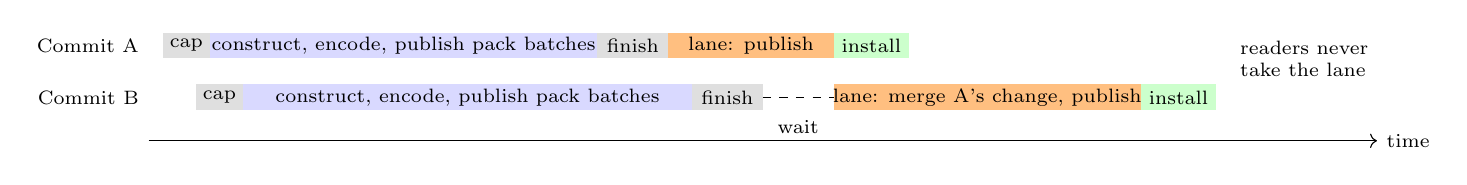
\begin{tikzpicture}[font=\scriptsize,x=0.6cm,y=0.55cm]
\draw[->] (0,0) -- (26,0) node[right]{time};
% Commit A
\node[anchor=east] at (0,2.2) {Commit A};
\fill[gray!25] (0.3,1.9) rectangle (1.3,2.5); \node at (0.8,2.2) {cap};
\fill[blue!15] (1.3,1.9) rectangle (9.5,2.5); \node at (5.4,2.2) {construct, encode, publish pack batches};
\fill[gray!25] (9.5,1.9) rectangle (11,2.5); \node at (10.25,2.2) {finish};
\fill[orange!50] (11,1.9) rectangle (14.5,2.5); \node at (12.75,2.2) {lane: publish};
\fill[green!20] (14.5,1.9) rectangle (16.1,2.5); \node at (15.3,2.2) {install};
% Commit B
\node[anchor=east] at (0,1.0) {Commit B};
\fill[gray!25] (1,0.7) rectangle (2,1.3); \node at (1.5,1.0) {cap};
\fill[blue!15] (2,0.7) rectangle (11.5,1.3); \node at (6.75,1.0) {construct, encode, publish pack batches};
\fill[gray!25] (11.5,0.7) rectangle (13,1.3); \node at (12.25,1.0) {finish};
\draw[dashed] (13,1.0) -- (14.5,1.0); \node[below] at (13.75,0.7) {wait};
\fill[orange!50] (14.5,0.7) rectangle (21,1.3); \node at (17.75,1.0) {lane: merge A's change, publish};
\fill[green!20] (21,0.7) rectangle (22.6,1.3); \node at (21.8,1.0) {install};
\node[anchor=west,align=left] at (22.9,1.9) {readers never\\take the lane};
\end{tikzpicture}
\caption{Two concurrent Commits on one Branch. Construction, compression and pack
batches overlap; only the lane serializes, and B merges only the change A published.}
\label{fig:twocommits}
\end{figure}

\paragraph{Read path.} A read that misses the kernel page cache (1) arrives as a FUSE
request of at most 128\,KiB, with one background request outstanding; (2) runs one
overlay job under the \ws{} lock that decides locally written bytes; (3) reads inherited
bytes \emph{outside} that lock from the shared object cache; (4) on a miss, issues one
batched Store demand, plus 8\,MiB of read-ahead for sequential streams (at most 16\,MiB
held per reader); and (5) decodes delta bases and zstd frames through a 2\,MiB pack
cache, re-hashing every object against its identifier. Mount reads only the root object.
Per-request round trips and decoding, not history depth, dominate read cost.

\paragraph{Lifecycles and custody.} A Sandbox lives from creation until it is explicitly
closed or its machine stops. A \ws{} is mounted, serves any number of processes and
Commits, and is unmounted; unmount refuses uncommitted changes unless told to discard
them. A Commit ends \texttt{Committed} (possibly after merging a moved head),
\texttt{UpToDate}, \texttt{Conflict} (marker blocks become the \ws{}'s local base and the
next Commit is refused while complete markers remain), or uncertain. Every hop makes one
attempt; a lost reply is reported as unknown and its custody (published outcome,
captured reader, operation intent) is retained until inspected. Committed history
survives a daemon or Sandbox loss, which loses only the disposable overlays. Under the
only permitted SQLite profile (WAL, \texttt{synchronous=OFF}) the Store survives process
termination, but a kernel or VM crash can lose or damage it.

% ---------------------------------------------------------------------------
\section{Committed State: Objects, Trees and Packs}
\label{app:objects}

All committed state of a Store lives in one SQLite file or PostgreSQL schema as two kinds
of data: immutable, content-addressed \emph{objects} that encode filesystem trees, and a
small set of mutable \emph{history} rows that name tree roots.

\paragraph{Objects.} Every object is a canonical byte string in a fixed envelope
(Table~\ref{tab:layouts}). Its identifier is
$\mathrm{BLAKE3}(\texttt{"layerfs/object/v2\textbackslash 0"} \,\|\, \text{canonical
bytes})$, 32 bytes. The value begins with an 8-byte role magic, so equal payload bytes
under different roles have different identifiers. Thirteen roles exist: whole file,
chunk, extent leaf and branch, file state, inode leaf and branch, directory leaf and
branch, filesystem root, attribute leaf and branch, and symlink. Identity-bearing integers
are big-endian. Decoders refuse padding, trailing bytes, nonzero flags, unknown versions
and unsorted rows rather than repairing them, so each logical value has exactly one
encoding, and references are always derived from the bytes, never supplied by a caller.

\begin{table}[h]
\centering
\small
\begin{tabular}{l p{0.7\linewidth}}
\toprule
Structure & Layout (bytes) \\
\midrule
Envelope (13) & \texttt{"LFSO"} [0:4] $\cdot$ kind \texttt{0x01} [4] $\cdot$ payload\_len u32 [5:9] $=$ value\_len$+4$ $\cdot$ value\_len u32 [9:13] $\cdot$ value \\
Tree-page header (31) & magic [0:8] $\cdot$ version u16 $\cdot$ role $\cdot$ level $\cdot$ flags$=0$ $\cdot$ count u16 $\cdot$ two subtree totals u64 \\
Whole file & \texttt{"LFS5SML\textbackslash 0"} $\cdot$ version u16 $\cdot$ payload (canonical $=$ raw $+$ 23) \\
Chunk & \texttt{"LFS4CHK\textbackslash 0"} $\cdot$ payload $\leq$ 32,768 \\
File state (93) & \texttt{"LFS4MAP\textbackslash 0"} $\cdot$ version $\cdot$ length u64 $\cdot$ extents u64 $\cdot$ level $\cdot$ profile id (32) $\cdot$ mapping root (32) \\
Extent leaf entry (40) & chunk id (32) $\cdot$ offset into chunk u32 $\cdot$ length u32 \\
Extent branch entry (48) & cumulative end bytes u64 $\cdot$ cumulative end extents u64 $\cdot$ child id (32) \\
Inode value (73) & kind (bit 7 $=$ inline) $\cdot$ link count u64 $\cdot$ content root (32) $\cdot$ \{attribute root (32) $|$ mode u32 $\cdot$ mtime s i64 $\cdot$ ns u32 $\cdot$ 16 zero\} \\
Filesystem root (116) & \texttt{"LFS6FSR\textbackslash 0"} $\cdot$ version $\cdot$ role $\cdot$ profile id (32) $\cdot$ scope id (32) $\cdot$ root serial u64 $\cdot$ inode-table root (32) \\
\bottomrule
\end{tabular}
\caption{Canonical byte layouts.}
\label{tab:layouts}
\end{table}

\paragraph{Trees.} A filesystem root names an inode table: a B$^+$-tree keyed by 64-bit
serial whose leaves hold 50--100 rows of (serial, 73-byte inode value) and whose
branches hold 64--127 (maximum serial, child) rows. A directory's content root is its own
B$^+$-tree from raw-byte name to serial; a name binds a serial, never an object, so a
hard link is two names for one serial. Tree pages are at most 8,192 bytes, and directory
and attribute pages are at least 40\% full except at the root. A regular file below the
cutoff (128\,KiB by default) is one whole-file object; a larger file is a file state over
an extent B$^+$-tree of 64--128 entries per page whose leaves map logical ranges to
\emph{slices}---(chunk, offset, length)---of content-defined chunks
(Figure~\ref{fig:tree}). Slices let a localized edit keep the untouched parts of boundary
chunks, and cumulative totals in branch entries locate an offset with one binary search
per level. Holes are not special: a run of zeros is a sequence of identical all-zero
32\,KiB chunks whose identical mapping pages are shared by identity. Profile identities
hashed from the frozen chunking and page parameters are embedded in each file state and
root and checked on decode. Updates rewrite only root-to-change paths; every unread
subtree keeps its identity.

\begin{figure}[h]
\centering
\small
\begin{verbatim}
FilesystemRoot --> InodeLeaf (root page of the inode table)
                    1: Dir   --> DirectoryLeaf { "a.bin" -> 2, "b.txt" -> 3 }
                    2: File  --> FileState(len, extents, level 1, profile)
                    3: File  --> WholeFile "LFS5SML\0" | bytes
FileState --> ExtentBranch [(end0,n0,L0) (end1,n1,L1)]
                L0 ExtentLeaf [(C1,0,len1) (C2,0,len2) ...]      (64-128 entries)
                L1 ExtentLeaf [(C2,4096,len) (C9,0,len9) ...]    <- a slice of C2
                     |
                Chunk C1, C2, C9 ...   (shared across files, versions, Branches, projects)
\end{verbatim}
\caption{One directory and one chunked file.}
\label{fig:tree}
\end{figure}

\paragraph{Physical records.} Identity excludes physical form. Payload objects (whole
files and chunks) are stored as \texttt{FULL} (a zstd frame), \texttt{STORED} (raw bytes,
chosen by an incompressibility probe) or \texttt{PREFIX} (a zstd frame compressed against
one base object's payload, recording the 32-byte base identifier). Inode branches and
directory and extent pages may be stored as a COPY/INSERT program against a predecessor
page (\texttt{COPY} $=$ 0 $\cdot$ offset u32 $\cdot$ length u32; \texttt{INSERT} $=$ 1
$\cdot$ length u32 $\cdot$ bytes), kept only when strictly smaller. Inode leaves are
pooled: each 73-byte value is replaced by a 4-byte ordinal, and values live in
append-only, field-packed blocks of at most 4,000 bytes and 255 entries ending in a
CRC32C. Every read rebuilds canonical bytes, base first along a delta chain, and hashes
each element against its identifier.

\paragraph{Packs.} Records are grouped (at most 8,191 records and 64\,KiB per group) into
immutable packs of at most 256\,KiB in four lanes: ordinary (tree pages, optionally
zstd-compressed per group), chunk, whole file, and singleton for one record too large for
a pack. A pack is a 24-byte header (\texttt{"LFPACK"}, version, group count, used
length), a directory of group offsets, encoded and decoded lengths and codecs, and the
group bodies; its key is the SHA-256 of its sealed bytes. A locator row maps each object
identifier to (role, canonical length, pack, group, record).

\begin{table}[h]
\centering
\small
\begin{tabular}{p{0.08\linewidth} p{0.24\linewidth} p{0.40\linewidth} p{0.18\linewidth}}
\toprule
Group & Table & Key $\rightarrow$ contents & Written by \\
\midrule
Physical & \texttt{pack} & pack id $\rightarrow$ SHA-256, length, body (update and delete refused by trigger) & object batches \\
 & \texttt{object\_location} & object id $\rightarrow$ role, canonical length, pack, group, record & object batches (insert if absent) \\
 & \texttt{inode\_value\_block} & first ordinal $\rightarrow$ $\leq$255 packed values $+$ CRC32C & object batches \\
 & \texttt{content\_signature} & ring slot $\rightarrow$ object id, 32-byte sketch & object batches (upsert) \\
 & \texttt{store\_policy}, \texttt{store\_totals} & cutoff, depth caps, next pack id and ordinal; byte totals & reservation, publication \\
History & \texttt{layer\_stack} & id $\rightarrow$ name, scope, profile, head Layer & init, \texttt{add\_layer} \\
 & \texttt{layer} & id $\rightarrow$ stack, parent, root, source Branch and Commit & \texttt{add\_layer} \\
 & \texttt{commit} & id $\rightarrow$ root, parent(s), base Layer, message, statistics, \texttt{.lww} decisions & publication lane \\
 & \texttt{branch} & id $\rightarrow$ name, base Layer, forked-from node, head Commit & fork, merge, lane \\
 & \texttt{scope\_allocator} & scope $\rightarrow$ serial high-water mark & serial reservation \\
Lineage & \texttt{layer\_lineage}, \texttt{commit\_lineage}, \ldots & heights, first-parent runs, absorption & with each Layer or Commit \\
Hints & \texttt{binding\_hint\_block}, \texttt{file\_digest} & name-binding hints; file-bytes digest $\rightarrow$ root & before the lane \\
\bottomrule
\end{tabular}
\caption{Store tables (SQLite; PostgreSQL is equivalent). Object batches run outside the
publication lane; only Commit insertion and head moves run inside it.}
\label{tab:schema}
\end{table}

\paragraph{History and invariants.} History identifiers are domain-separated BLAKE3
digests with a one-byte kind tag; a Commit identifier covers its root, parents, base
Layer and message but not its timestamp. Lineage tables record each Commit's
first-parent run and depth, so ancestry queries walk run segments rather than individual
Commits. The Store maintains six invariants: (i) every read authenticates; (ii) one
encoding per value; (iii) references are derived from bytes; (iv) packs, locators and
value blocks are append-only; (v) pack identifiers and inode serials are never reused;
(vi) Commits and Layers are immutable, and only Branch and stack heads move, by
expected-head checks. (Mutable rows besides heads are counters, the similarity ring and
the file-digest hint table.)

% ---------------------------------------------------------------------------
\section{Workspace Overlay and Request Path}
\label{app:overlay}

\paragraph{Overlay database.} Each mounted \ws{} owns one SQLite file created by a byte
copy of a schema-only template built at daemon start; mount therefore costs a fixed-size
file copy and one root-object read, independent of the tree. The file runs a disposable
profile (\texttt{journal\_mode=MEMORY}, \texttt{synchronous=OFF},
\texttt{locking\_mode=EXCLUSIVE}, 4\,KiB pages, no mmap, \texttt{busy\_timeout=0}) and
holds only changes (Table~\ref{tab:overlay}). All tables are \texttt{STRICT}; all except
the payload table and two single-key tables are \texttt{WITHOUT ROWID}. \texttt{fs\_data}
keeps a rowid so live runs can be overwritten in place with incremental blob I/O.

\begin{table}[h]
\centering
\small
\begin{tabular}{p{0.30\linewidth} p{0.62\linewidth}}
\toprule
Table & Rows \\
\midrule
\texttt{fs\_inode(inode, generation)} & One row per changed inode per generation: size, mode, mtime, kind, \texttt{inherited\_cutoff} \\
\texttt{fs\_entry(parent, name, generation)} & One row per changed name; a NULL inode is a whiteout \\
\texttt{fs\_data} & File bytes as 4\,KiB cells with a per-byte validity mask, or dense runs of whole cells inside one aligned 32\,KiB slot \\
\texttt{fs\_data\_ref} & \emph{Reference pieces}: ranges declared equal to committed bytes of a content root; no bytes stored \\
\texttt{fs\_truncate} & A shrink ``staircase'' so stale cells can be identified by epoch \\
\texttt{fs\_predecessor} & The file a rename replaced; an advisory delta base for the next Commit \\
\texttt{fs\_digest}, \texttt{cleanup\_task} & Append-only BLAKE3 digests; the reclamation queue \\
\bottomrule
\end{tabular}
\caption{Overlay schema (selected tables).}
\label{tab:overlay}
\end{table}

\paragraph{Layered view.} A \ws{}'s view is the committed base root plus overlay rows
with $\mathit{installed} < \mathit{generation} \leq \mathit{active}$. Each inode row
carries an \texttt{inherited\_cutoff}: bytes below it not written in that generation fall
through to the next lower layer and finally to the base file. Reads compose at most four
local layers newest-first and return the locally decided bytes, an \emph{inherited}
bitmask with one covering span, and reference ranges; the request then reads the span
and ranges from the immutable Store \emph{after} releasing the \ws{} lock.

\begin{figure}[h]
\centering
\resizebox{\linewidth}{!}{% Layered view of one file and the generation counters. Input by appendix.tex.
\begin{tikzpicture}[font=\scriptsize, x=1cm, y=1cm,
  cell/.style={draw, fill=orange!55, minimum height=0.42cm, inner sep=0},
  ref/.style={draw, pattern=north east lines, pattern color=blue!60, minimum height=0.42cm},
  ext/.style={draw, fill=gray!18, minimum height=0.42cm, inner sep=0},
  lbl/.style={anchor=east, align=right, font=\scriptsize},
  ar/.style={-{Stealth[length=4pt]}, thick}]
% ---------------- panel (a)
\node[font=\scriptsize\bfseries, anchor=west] at (-2.6,3.55) {(a) One file seen through the overlay};
% base file: committed extents (chunk slices)
\node[lbl] at (-0.15,0) {base file\\(committed root)};
\foreach \a/\b/\n in {0/1.6/c1, 1.6/2.9/c2, 2.9/4.7/c3, 4.7/5.9/c4, 5.9/7.6/c5, 7.6/9.0/c6}{
  \draw[fill=gray!18] (\a,-0.21) rectangle (\b,0.21); \node at ({(\a+\b)/2},0) {\n};}
% captured generation g
\node[lbl] at (-0.15,1.1) {generation $g$\\(captured)};
\draw[dotted] (0,0.89) rectangle (9.0,1.31);
\draw[fill=orange!55] (2.0,0.89) rectangle (2.25,1.31);
\draw[pattern=north east lines, pattern color=blue!60] (5.0,0.89) rectangle (6.6,1.31);
\node[font=\scriptsize, above] at (5.8,1.31) {reference piece};
\node[font=\scriptsize, above] at (2.12,1.31) {cell};
% active generation g+1, after a truncate and re-extension
\node[lbl] at (-0.15,2.2) {generation $g{+}1$\\(active)};
\draw[dotted] (0,1.99) rectangle (8.2,2.41);
\draw[fill=orange!55] (3.3,1.99) rectangle (4.1,2.41);
\node[font=\scriptsize, above] at (3.7,2.41) {32\,KiB run};
\draw[very thick, red!70!black] (7.0,1.85) -- (7.0,2.55);
\node[font=\scriptsize, red!70!black, above] at (7.0,2.55) {cutoff};
\fill[white] (7.0,1.99) rectangle (8.2,2.41);
\draw[dotted] (7.0,1.99) rectangle (8.2,2.41);
\node[font=\scriptsize] at (7.6,2.2) {zeros};
% composed view
\node[lbl] at (-0.15,-1.2) {what READ\\returns};
\foreach \a/\b/\c in {0/2.0/gray!18, 2.0/2.25/orange!55, 2.25/3.3/gray!18, 3.3/4.1/orange!55, 4.1/5.0/gray!18, 7.0/8.2/white}{
  \draw[fill=\c] (\a,-1.41) rectangle (\b,-0.99);}
\draw[pattern=north east lines, pattern color=blue!60] (5.0,-1.41) rectangle (6.6,-0.99);
\draw[fill=gray!18] (6.6,-1.41) rectangle (7.0,-0.99);
\node[font=\scriptsize] at (7.6,-1.2) {zeros};
\draw[decorate, decoration={brace, amplitude=3pt, mirror}] (0,-1.5) -- (8.2,-1.5)
  node[midway, below=3pt, font=\scriptsize, align=center] {one job under the \ws{} lock decides orange and zero bytes;\\gray and hatched bytes are read from the Store after it is released};
\draw[ar] (9.45,2.3) -- node[right, align=left, font=\scriptsize] {newest\\first} (9.45,0.0);
% ---------------- panel (b)
\begin{scope}[xshift=10.5cm]
\node[font=\scriptsize\bfseries, anchor=west] at (-0.3,3.55) {(b) Generation counters};
\draw[->] (0,2.4) -- (5.0,2.4) node[right] {gen};
\foreach \x/\t in {0.8/installed, 2.3/captured, 3.8/active}{
  \draw (\x,2.3) -- (\x,2.5); \node[above, font=\scriptsize] at (\x,2.5) {\t};}
\node[align=left, anchor=north west, text width=5.2cm] at (-0.3,2.0) {
\textbf{Visible rows}: $\mathit{installed} < \mathit{gen} \leq \mathit{active}$.\\[2pt]
\textbf{Capture} (Commit start): seal \emph{active} as \emph{captured};
new writes go to $\mathit{active}{+}1$. No row is copied.\\[2pt]
\textbf{Construct}: read only the sealed generation, in pages of $\leq$1,024 rows.\\[2pt]
\textbf{Install} (after publish): base root $\gets$ new root;
$\mathit{installed} \gets \mathit{captured}$ in one SQL step.\\[2pt]
\textbf{Reclaim}: rows at or below the floor are deleted after the reply, in small steps.};
\end{scope}
\end{tikzpicture}
}
\caption{(a) A file seen through the overlay: two generations of rows over the committed file. A READ composes them newest first, deciding locally written and zero bytes under the \ws{} lock and reading inherited and referenced bytes from the Store after releasing it. (b) Capture and install move counters, not rows.}
\label{fig:overlayview}
\end{figure}

\paragraph{Request path.} All state of one \ws{} sits behind one mutex. A job holds it
for at most one transaction and performs no Store I/O; base facts a job lacks are
returned as \emph{needs}, read without the lock, and supplied to a second job that
decides over the then-current rows. Kernel lookup counts, open descriptors, directory
cookies and read windows live in in-memory maps that commit or roll back with the job's
SQL. Windows bound each job, not files: a FUSE WRITE carries at most 128\,KiB (the
negotiated \texttt{max\_write}; the 256\,KiB job window is the NFS transfer size), a read
at most 128\,KiB, a page of rows at most 1,024. Algorithms~\ref{alg:write}
and~\ref{alg:read} show WRITE and READ.

\begin{algorithm}[h]
\caption{FUSE WRITE$(s, \mathit{off}, d)$, $|d| \leq 128$\,KiB}
\label{alg:write}
\small
\begin{algorithmic}[1]
\State $\mathit{claims} \gets$ \Call{Recognize}{$s, \mathit{off}, d$} \Comment{optional, bounded, no lock}
\Loop
  \State lock($W$) \Comment{one job, at most one transaction}
  \State $o \gets$ newest row of $s$ with generation in $(\mathit{installed}, \mathit{active}]$, else base facts
  \If{$o$ unknown} unlock; fetch base inode of $s$ without the lock; \textbf{continue} \EndIf
  \State \textbf{begin}; if no row $(s, \mathit{active})$, insert one with cutoff $\gets o.\mathit{size}$
  \ForAll{32\,KiB slots overlapping $[\mathit{off}, \mathit{off}+|d|)$}
    \State whole cells: overwrite the live dense run in place, or replace it with one run
    \State partial cell: point read, merge, set validity bits \Comment{no base read}
  \EndFor
  \State cells in $\mathit{claims}$ $\rightarrow$ reference pieces (no bytes)
  \State size $\gets \max(o.\mathit{size}, \mathit{off}+|d|)$; revision $\mathrel{+}= 1$; \textbf{commit}; unlock
  \State reply $|d|$; \textbf{return}
\EndLoop
\end{algorithmic}
\end{algorithm}

\begin{algorithm}[h]
\caption{FUSE READ$(s, \mathit{off}, n)$, $n \leq 128$\,KiB}
\label{alg:read}
\small
\begin{algorithmic}[1]
\State lock($W$) \Comment{read-only job}
\State $L \gets$ newest $\leq 4$ rows of $s$ with generation in $(\mathit{installed}, \mathit{active}]$
\ForAll{$\ell \in L$, newest first}
  \State copy live cells and runs of $\ell$ into undecided bytes
  \State mark bytes covered by $\ell$'s reference pieces as reference ranges
  \State mark bytes $\geq \ell.\mathit{cutoff}$ below EOF decided (zero if unwritten)
\EndFor
\State $r \gets$ base root at this instant; unlock
\If{every byte decided} reply \EndIf
\State read the inherited span of the base file at $r$ and the reference ranges \Comment{outside the lock}
\State reply
\end{algorithmic}
\end{algorithm}

\paragraph{No copy-up.} The first write to a committed file inserts one inode row whose
cutoff is the base length and stores only the written cells; no base byte is read or
copied, and partially written cells keep unwritten bytes inherited through their masks.
A truncate edits at most one 32\,KiB row, adds one staircase step and lowers the cutoff.
Appends past the old length skip even the row-shape read. Renames, including directory
renames and rename-over, change at most four inode rows and two name rows and move no
bytes; a rename-over records the replaced file as a predecessor. Hard links share one
serial and hence one kernel inode.

\paragraph{Capture and install.} A Commit seals the active generation by an in-memory
state change: \emph{active} becomes \emph{captured} and new mutations go to
$\mathit{active}+1$; no row is copied. Capture waits until every earlier mutation's reply
has been attempted, and later mutations wait behind it, so the captured frontier is
finite. Construction reads only the sealed generation, in pages of at most 1,024 rows.
After publication, install is one SQL step that sets the new base root and raises the
floor to the captured generation, plus a pointer swap of the base view; no tree is
walked. Rows written after the capture remain on top of the view, because their cutoffs
were taken from the sealed layer that the new root reproduces. Rows of the retired
generation are deleted after the Commit replies, in steps of at most 14 cells or 64 rows.

\begin{table}[h]
\centering
\small
\begin{tabular}{p{0.20\linewidth} p{0.22\linewidth} p{0.24\linewidth} p{0.12\linewidth} p{0.10\linewidth}}
\toprule
Operation & Overlay cost & Base cost & In tree size & In file size \\
\midrule
Mount & fixed template copy & one root object & $O(1)$ & -- \\
LOOKUP, GETATTR & $O(\log R)$ & $O(\log D + \log N)$ pages if unchanged & logarithmic & $O(1)$ \\
READ $w$ & $O(w + L\log R)$ & $O(w) + O(\log F)$ mapping pages & $O(1)$ & logarithmic \\
WRITE $w$ & $O(w + \log R)$ & none & $O(1)$ & $O(1)$ \\
Truncate & one $\leq$32\,KiB row $+ O(\log h)$ & none & $O(1)$ & $O(1)$ \\
CREATE, UNLINK, RENAME, LINK & $\leq$4 inode $+$ $\leq$2 name rows & name facts & $O(1)$ rows & $O(1)$ \\
Capture, install & in memory / one SQL step & one root object & $O(1)$ & $O(1)$ \\
\bottomrule
\end{tabular}
\caption{Per-request cost. $R$ changed rows, $N$ inodes, $D$ directory entries, $F$ file
size, $L \leq 4$ layers, $h$ staircase height. Logarithmic base costs follow from the
B$^+$-tree layout.}
\label{tab:overlaycost}
\end{table}

\paragraph{Limits.} Kernel write-back caching is off, so each \texttt{write(2)} is a
synchronous FUSE WRITE published to the overlay, and dirty shared-mapping pages not yet
sent are outside a capture. FLUSH and FSYNC answer \texttt{ENOSYS} once: durability
exists only at Commit. Extended attributes, READDIRPLUS, remote locks, \texttt{fallocate}
and \texttt{copy\_file\_range} are not implemented. Per-\ws{} open state (lookups,
descriptors, readers) is the one resident structure without a cap.

% ---------------------------------------------------------------------------
\IfFileExists{appendix-pipeline.tex}{% Input by appendix.tex. Notes: notes/appendix/P-pipeline.md.
\section{From \texttt{write(2)} to Stored Bytes}
\label{app:pipeline}

\sys{} turns filesystem calls into Store objects in two phases. At write time it records
\emph{what changed}, cheaply and without reading committed data. At Commit time it turns
that record into the smallest set of new immutable objects it can find in bounded work.
This appendix follows one byte range through content addressing, chunking, deduplication,
compression and delta encoding. Measurements are the evaluation's single samples
(Section~\ref{sec:eval}); stored bytes are exact.

\begin{figure}[h]
\centering
\resizebox{\linewidth}{!}{% write(2) -> stored bytes pipeline. Input by appendix-pipeline.tex.
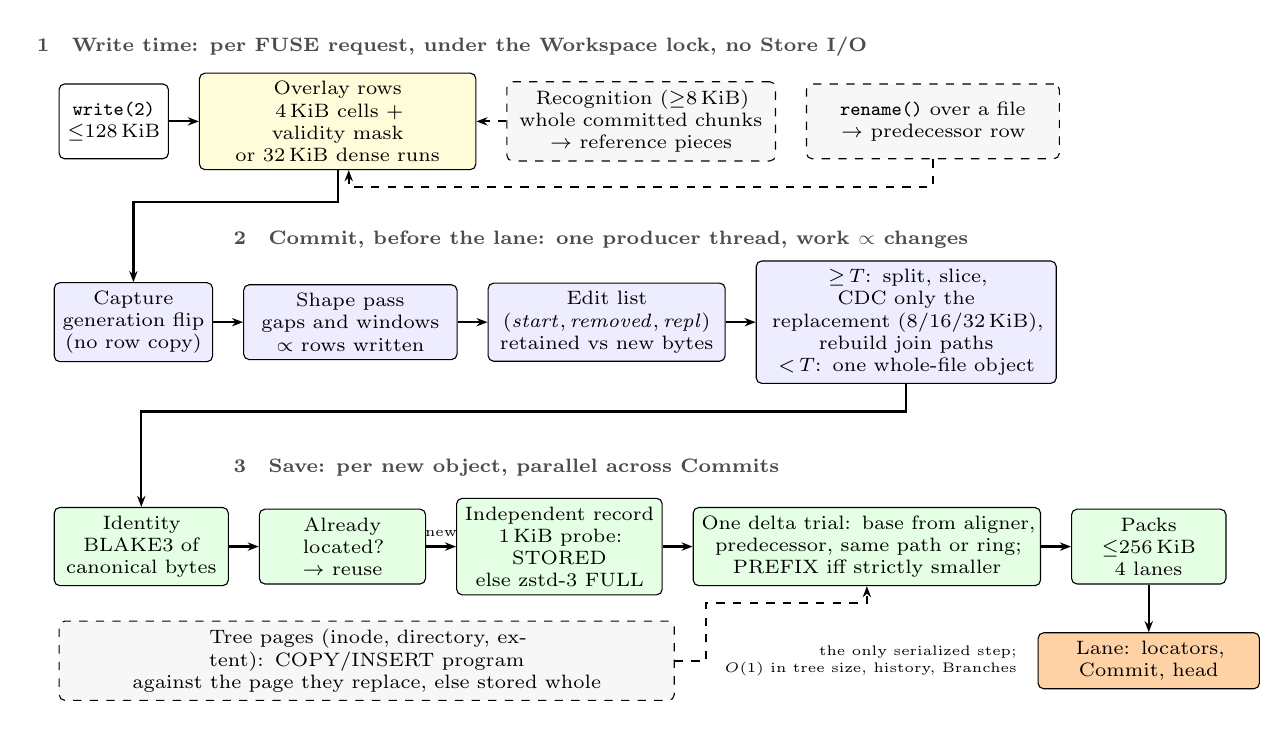
\begin{tikzpicture}[
  font=\scriptsize,
  box/.style={draw, rounded corners=2pt, align=center, inner sep=3pt, minimum height=0.95cm, fill=white},
  st/.style={box, fill=blue!7},
  ov/.style={box, fill=yellow!15},
  sv/.style={box, fill=green!10},
  ln/.style={box, fill=orange!35},
  side/.style={box, dashed, fill=gray!6},
  ar/.style={-{Stealth[length=4pt]}, thick},
  lane/.style={font=\scriptsize\bfseries, anchor=west, text=black!70},
  node distance=0.32cm and 0.38cm
]
% ---- row 1: write time
\node[lane] (l1) at (-0.2,0.95) {1\;\; Write time: per FUSE request, under the \ws{} lock, no Store I/O};
\node[box] (w) at (0.9,0) {\texttt{write(2)}\\$\leq$128\,KiB};
\node[ov, right=of w, text width=3.3cm] (cells) {Overlay rows\\4\,KiB cells $+$ validity mask\\or 32\,KiB dense runs};
\node[side, right=of cells, text width=3.2cm] (rec) {Recognition ($\geq$8\,KiB)\\whole committed chunks\\$\rightarrow$ reference pieces};
\node[side, right=of rec, text width=3.0cm] (pred) {\texttt{rename()} over a file\\$\rightarrow$ predecessor row};
\draw[ar] (w) -- (cells);
\draw[ar,dashed] (rec) -- (cells);
\draw[ar,dashed] (pred.south) |- ++(0,-0.35) -| ([xshift=4pt]cells.south);
% ---- row 2: commit, before the lane
\node[lane] (l2) at (2.3,-1.5) {2\;\; Commit, before the lane: one producer thread, work $\propto$ changes};
\node[st, text width=1.8cm] (cap) at (1.15,-2.55) {Capture\\generation flip\\(no row copy)};
\node[st, right=of cap, text width=2.5cm] (shape) {Shape pass\\gaps and windows\\$\propto$ rows written};
\node[st, right=of shape, text width=2.8cm] (edits) {Edit list\\$(\mathit{start}, \mathit{removed}, \mathit{repl})$\\retained vs new bytes};
\node[st, right=of edits, text width=3.6cm] (build) {$\geq$\,$T$: split, slice, CDC only the\\replacement (8/16/32\,KiB),\\rebuild join paths\\$<$\,$T$: one whole-file object};
\draw[ar] (cells.south) -- ++(0,-0.4) -| (cap.north);
\draw[ar] (cap) -- (shape);
\draw[ar] (shape) -- (edits);
\draw[ar] (edits) -- (build);
% ---- row 3: Save
\node[lane] (l3) at (2.3,-4.4) {3\;\; Save: per new object, parallel across Commits};
\node[sv, text width=2.0cm] (id) at (1.25,-5.4) {Identity\\BLAKE3 of\\canonical bytes};
\node[sv, right=of id, text width=1.9cm] (dedup) {Already\\located?\\$\rightarrow$ reuse};
\node[sv, right=of dedup, text width=2.4cm] (ind) {Independent record\\1\,KiB probe: STORED\\else zstd-3 FULL};
\node[sv, right=of ind, text width=4.2cm] (delta) {One delta trial: base from aligner,\\predecessor, same path or ring;\\PREFIX iff strictly smaller};
\node[sv, right=of delta, text width=1.75cm] (pack) {Packs\\$\leq$256\,KiB\\4 lanes};
\draw[ar] (build.south) -- ++(0,-0.35) -| (id.north);
\draw[ar] (id) -- (dedup);
\draw[ar] (dedup) -- node[above,font=\tiny]{new} (ind);
\draw[ar] (ind) -- (delta);
\draw[ar] (delta) -- (pack);
% ---- row 4: pages and lane
\node[side, text width=7.6cm, minimum height=0.6cm, anchor=west] (pages) at (0.2,-6.85) {Tree pages (inode, directory, extent): COPY/INSERT program\\against the page they replace, else stored whole};
\node[ln, text width=2.6cm, minimum height=0.6cm] (lane) at (pack |- pages) {Lane: locators,\\Commit, head};
\draw[ar] (pack) -- (lane);
\draw[ar, dashed] (pages.east) -- ++(0.4,0) |- ([yshift=-6pt]delta.south) -- ([yshift=0pt]delta.south);
\node[font=\tiny, anchor=east, align=right] at ([xshift=-4pt]lane.west) {the only serialized step;\\$O(1)$ in tree size, history, Branches};
\end{tikzpicture}
}
\caption{From \texttt{write(2)} to stored bytes. Row 1 runs per request without Store I/O; rows 2 and 3 run before the publication lane, in parallel across Commits; only the lane is serialized.}
\label{fig:pipeline}
\end{figure}

\paragraph{Write time: localized-edit capture.} Kernel write-back is off, so every
\texttt{write(2)} reaches the daemon and is published into the \ws{}'s overlay
(Appendix~\ref{app:overlay}) before it returns. Bytes are kept as 4\,KiB cells, whose
per-byte validity mask distinguishes a written zero from a hole, or as dense runs of up
to 32\,KiB. Holes cost no rows, a shrink is one staircase row, and a write never reads
the committed bytes it partly covers. Two kinds of provenance are kept beside the bytes.
A \emph{reference piece} says that a range equals bytes of a committed file: \emph{write
recognition} creates one when a write of at least 8\,KiB contains whole chunks the file
already had, as when a program rewrites a file in place, and stops after 1\,MiB of
unmatched bytes. A \emph{predecessor} row records that \texttt{rename()} put one file
over another, which is how editors, Git and package managers save.

\paragraph{Capture to edit list.} A Commit seals the overlay generation without copying
rows. For each changed file a first pass reads only row \emph{shapes}: an unchanged
region is one indexed gap, so the pass grows with rows written, not with file length. A
one-pass script turns the spans into an ordered edit list in result coordinates. Bytes
inherited from the file's own base, or reference pieces of it, are \emph{retained};
everything else is new. Overwrites, appends (one trailing insert), truncations (one
trailing delete), holes (zero runs) and shifted rewrites (pieces plus a small residue,
with up to 64\,KiB at each edge compared against the base and trimmed where equal) all
come out in this one form, and a rewrite that reproduces the base exactly returns the
base root.

\paragraph{Construction.} Content applies the edits to the stored extent tree
(Algorithm~\ref{alg:edit}): it splits extents at each boundary, drops the replaced
middle unread, chunks only the replacement, and rebuilds pages only on the join paths.
Unchanged extents keep their chunk identities, possibly as slices. A file the base did
not hold---a new path, a renamed-over temporary file, a recreated path---is built from
scratch; because chunking is content-defined, its unchanged chunks resynchronize and are
the same objects as before. \emph{Small files} below the per-Store cutoff (128\,KiB by
default; any power of two up to 1\,MiB) are single whole-file objects, rebuilt whole on
every edit, so their natural delta base is the previous version of the whole file.

\paragraph{Storage.} Each object's identity is the BLAKE3 hash of its canonical bytes,
so identical files, chunks, pages and subtrees are stored once across Commits, Branches
and projects. The Save reuses any object already located, then gives each new payload
one representation trial (Algorithm~\ref{alg:select}). The independent record is a
level-3 zstd frame, or raw when a 1\,KiB probe saves at most 1/32. At most one delta base
is tried, and the delta is kept only if strictly smaller. Bases come from filesystem
events rather than search: the edited version, the aligned old chunk, the renamed-over
file or the file previously at the same path; a similarity sketch is the fallback for
whole files only. Tree pages get COPY/INSERT programs against the page they replace.
Chains are bounded in depth and decode work, and a chain that reaches a bound is
re-based onto its root. Records are grouped into append-only 256\,KiB packs inside the
single Store database; the ordinary lane compresses tree-page groups with zstd level~1.

\paragraph{The codec is frozen deliberately.} An offline study of 9,386 files under
128\,KiB found zstd-6 4.4\% smaller than zstd-3 at 2.6\X{} the compression CPU, a
trained dictionary 14\% smaller but requiring a new frame format, and 256\,KiB group
compression 22\% smaller but forcing 256\,KiB of decoding to serve a 2\,KB file.
\sys{} keeps per-object, random-access records and spends its effort on base selection
and metadata instead. The cost is visible: per-chunk frames lose cross-chunk context, so
64\,MiB of synthetic text stores 1.25\X{} larger than a whole-file \texttt{zstd -3}.

\begin{table}[h]
\centering
\small
\begin{tabular}{p{0.24\linewidth} p{0.33\linewidth} p{0.35\linewidth}}
\toprule
Workload pattern & Absorbed by & Measured \\
\midrule
Copy of a 50\,MB tree & File-digest relink, content addressing & Copy Commit of 500\,MB: 15.9\,KB, no payload; 11.9\X{} over 10 copies \\
Small text edit in place & Whole-file PREFIX delta against the edited version & delta$+$zstd 32.1\X{} (100 files, 20 Commits of 1\% edits) \\
Rename-over save, small file & Predecessor recorded at \texttt{rename()} & 32.0\X{}; payload equal to in-place editing \\
Rename-over save, large file & Content addressing $+$ aligned chunk bases & Git index churn $-$80\% (1.46\,MB $\rightarrow$ 0.30\,MB) \\
New path per version & Same-path base, similarity ring & 30.1\X{} \\
100\,B overwrite, 500\,MiB file & Cell row, one edit, one new chunk & 153\,B payload, 5.9\,KB stored per Commit \\
100\,B insert shifting a 10\,MiB tail & Recognition $\rightarrow$ reference pieces & 153\,B payload, 4.0\,KB metadata per Commit \\
16\,KiB append, 5\,MiB file & Trailing insert, losing-base back-off & 17.0\,KB per Commit ($+$0.3\% payload) \\
Truncate 500\,MiB to 0 & Split and discard & 8.4\,KB, metadata only \\
500\,MiB of random data & Raw after probe & $+$0.11\% payload \\
64\,MiB of zeros & Zero runs, repeated pages & 76\,B payload, 684\,B metadata \\
SQLite page churn & In-place page edits, chunk deltas & 13.7\X{} raw$\div$stored (a Git pack is 2.3\X{} smaller) \\
Tiny files & Whole-file objects, pooled metadata & 0.91\X{}: Store larger than raw \\
20 projects in one Store & Store-wide content addressing & 16.7\X{} smaller than 20 Stores \\
\bottomrule
\end{tabular}
\caption{Which mechanism absorbs which workload pattern.}
\label{tab:patterns}
\end{table}

\paragraph{Example 1: a 100-byte overwrite in a 500\,MiB file.} The write produces one
cell row in the overlay (two if it crosses a 4\,KiB boundary) and reads nothing from the
Store; recognition is skipped below 8\,KiB. At Commit the shape pass finds one local
window between two inherited gaps and emits a single overwrite edit. The edit reads the
mapping pages on the path to that offset---about 27,000 extents in a three-level tree,
by calculation---and the one stored chunk under the range, finds that the bytes differ,
splits the chunk's extent into two slices, scans the 100 bytes into one new chunk, and
rebuilds only that leaf, its ancestors and the 93-byte file state. Each rebuilt page is
offered its predecessor as a COPY/INSERT base, and the old overlapping chunk is offered
as the new chunk's delta base (random data stays raw). The parent directory is
untouched, because directory entries bind inode serials rather than content. Over five
Commits each stored 153\,B of payload and 5.7\,KB of metadata; the Store grew 7.4\,KB per
Commit and a cold Commit took 28\,ms, against 524\,MB and 0.6\,s for a whole-file
copy-up overlay. The same edit on 10\,MiB and 100\,MiB files stores the same 153\,B; in a
unit test, a larger file adds one page read per tree level (3 pages at 8\,MB, 4 at
24\,MB, the same three payloads).

\paragraph{Example 2: a rename-over save of a small file.} An editor writes
\texttt{f.tmp} (a new inode, say 40\,KiB) and calls \texttt{rename(f.tmp, f)}. The overlay
stores the new bytes as dense runs, rebinds the name \texttt{f} to the new serial and
records the old serial as its predecessor; no Store I/O happens. At Commit the new file
has no base of its own, so it is built from scratch as one whole-file object, and the
old file's root is declared as an explicit delta base without being read. The Save tries
one zstd frame with the old version as prefix (the 256\,KiB window covers both) and keeps
it if smaller. The directory page that maps \texttt{f} gets a COPY/INSERT program against
the page it replaces. On 100 such files with 1\% line edits, 20 Commits stored about
613\,B per file version (32.0\X{}, against 32.1\X{} for in-place editing); on a smaller
suite of 25 files the rename-over and in-place payloads are byte-identical. For a large
file saved this way, such as Git's index, the new file is re-chunked in full, unchanged
chunks dedupe by identity, and the aligner offers each new chunk the old chunk at the
same position: index churn fell 80\%, with 110 of 120 chunks stored as deltas.

\paragraph{Costs.} Tiny files cost about 200\,B each beyond their bytes, so a Store of
2\,KB files is about 10\% larger than the raw data. Metadata is about two-thirds of a
typical small Commit; fitted per-operation costs are 414\,B per edit, 1,360\,B per new
file, 1,111\,B per delete and 464\,B per rename. New data is written twice, once to the
overlay and again to the Store, so a 500\,MiB random write commits more slowly than in a
copy-up overlay (1.36\,s against 1.0\,s cold). A large file saved under a new inode is
re-chunked in full: storage stays small, but CPU does not, because recognition covers
only same-inode writes. Edits fragment the mapping into slices with no defragmentation,
and equal bytes may then have different roots, which is why diff and merge compare
bytes. Nothing is garbage-collected or repacked: removing a 500\,MiB file frees nothing
until a collector exists.
}{}

% ---------------------------------------------------------------------------
\section{Algorithms}
\label{app:algorithms}

\subsection{Content-defined chunking}

\sys{} uses a FastCDC-style GEAR scanner~\cite{fastcdc} with minimum 8\,KiB, target
16\,KiB and maximum 32\,KiB, two bytes per step, and normalization level~2: the cut
probability per byte is $2^{-16}$ between 8 and 16\,KiB and $2^{-12}$ between 16 and
32\,KiB. The first 8\,KiB of each chunk are copied without hashing. Scanner state
(chunk buffer, hash, and a pending odd byte) persists across reads, so read-buffer
boundaries never move a cut. The profile (sizes, masks, seed and table) is digested into
every file state.

\emph{Zero runs.} For a run of zeros the scanner state repeats with period 32\,KiB. A hole
of length $\ell$ is handled as one 32\,KiB scan, a repeat count $n = \lfloor(\ell -
32\,\mathrm{KiB})/32\,\mathrm{KiB}\rfloor$ of one all-zero chunk, and the remainder; the
mapping builder emits \emph{one} uniform page of 128 identical entries to stand for every
full page and recurses on the next level. A hole of any length therefore costs
$O(32\,\mathrm{KiB})$ scanning plus $O(h \cdot 128)$ mapping work for tree height $h =
O(\log_{128}(\ell/32\,\mathrm{KiB}))$, and yields the same partition and root as
byte-by-byte scanning.

\subsection{Localized edits and the aligner}

Edits are $(\mathit{start}, \mathit{removed}, \mathit{replacement})$ in result
coordinates. Algorithm~\ref{alg:edit} applies them to a chunked file. The removed middle
is discarded unread; only replacement bytes are chunked, with a fresh scanner, so CDC
never resynchronizes across an edit boundary and the two boundary chunks become slices.
Each edit costs two splits and two concatenations, each touching $O(h)$ pages on one
root-to-boundary path. The cost is therefore independent of file size: the same
overwrite reads 3 mapping pages on an 8\,MB file and 4 on a 24\,MB file.

\begin{figure}[h]
\centering
\resizebox{0.82\linewidth}{!}{% Localized edit on a file's extent tree: path copying with slices. Input by appendix.tex.
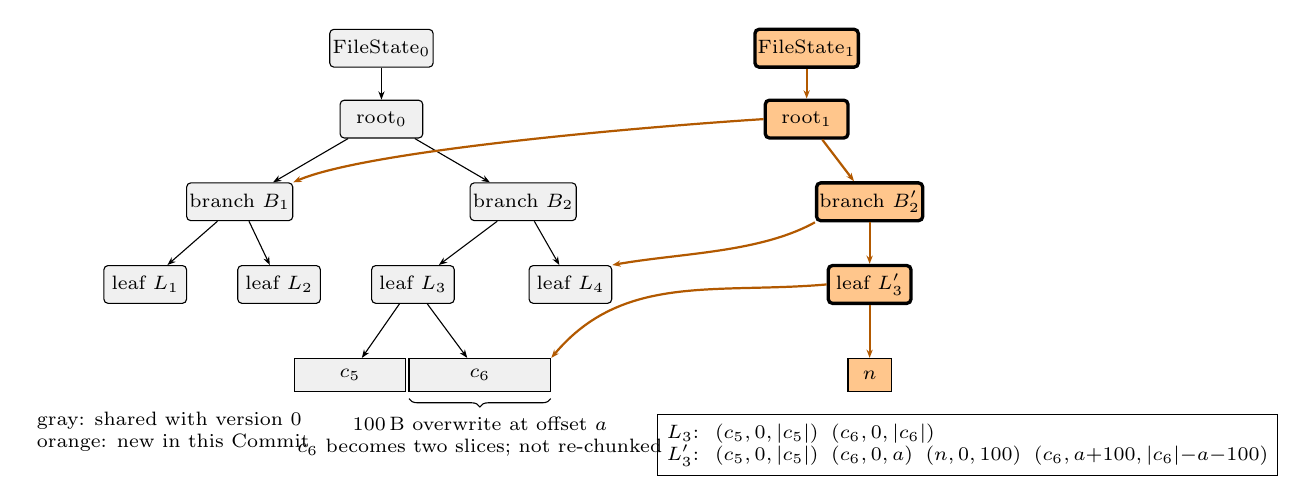
\begin{tikzpicture}[font=\scriptsize,
  pg/.style={draw, rounded corners=1.5pt, minimum width=1.05cm, minimum height=0.48cm, inner sep=1pt, fill=gray!12},
  nw/.style={pg, fill=orange!45, very thick},
  ch/.style={draw, minimum height=0.42cm, inner sep=1pt, fill=gray!12},
  chn/.style={ch, fill=orange!45},
  e/.style={-{Stealth[length=3pt]}},
  en/.style={-{Stealth[length=3pt]}, orange!70!black, thick}]
% old version (gray) and new version (orange) share every page off the edit path
\node[pg] (s0) at (3.2,3.2) {FileState$_0$};
\node[nw] (s1) at (8.6,3.2) {FileState$_1$};
\node[pg] (r0) at (3.2,2.3) {root$_0$};
\node[nw] (r1) at (8.6,2.3) {root$_1$};
\node[pg] (b1) at (1.4,1.25) {branch $B_1$};
\node[pg] (b2) at (5.0,1.25) {branch $B_2$};
\node[nw] (b2n) at (9.4,1.25) {branch $B_2'$};
\foreach \i/\x in {1/0.2,2/1.9,3/3.6,4/5.6}{\node[pg] (l\i) at (\x,0.2) {leaf $L_\i$};}
\node[nw] (l3n) at (9.4,0.2) {leaf $L_3'$};
\draw[e] (s0) -- (r0); \draw[e] (r0) -- (b1); \draw[e] (r0) -- (b2);
\draw[e] (b1) -- (l1); \draw[e] (b1) -- (l2); \draw[e] (b2) -- (l3); \draw[e] (b2) -- (l4);
\draw[en] (s1) -- (r1); \draw[en] (r1) -- (b2n); \draw[en] (b2n) -- (l3n);
\draw[en] (r1.west) .. controls (6.5,2.2) and (3.0,1.9) .. (b1.north east);
\draw[en] (b2n.south west) .. controls (8.0,0.6) and (7.0,0.6) .. (l4.north east);
% chunks under L3 and L3'
\node[ch, minimum width=1.4cm] (k5) at (2.8,-0.95) {$c_5$};
\node[ch, minimum width=1.8cm] (k6) at (4.45,-0.95) {$c_6$};
\draw[e] (l3) -- (k5); \draw[e] (l3) -- (k6);
\node[chn, minimum width=0.55cm] (n) at (9.4,-0.95) {$n$};
\draw[en] (l3n.south) -- (n);
\draw[en] (l3n.west) to[out=185,in=50] (k6.north east);
% leaf entries
\node[draw, fill=white, anchor=north west, align=left, font=\scriptsize] at (6.7,-1.45) {
$L_3$:\; $(c_5, 0, |c_5|)\;\; (c_6, 0, |c_6|)$\\
$L_3'$:\; $(c_5, 0, |c_5|)\;\; (c_6, 0, a)\;\; (n, 0, 100)\;\; (c_6, a{+}100, |c_6|{-}a{-}100)$};
\draw[decorate, decoration={brace, amplitude=3pt, mirror}] (3.55,-1.25) -- (5.35,-1.25)
  node[midway, below=3pt, font=\scriptsize, align=center] {100\,B overwrite at offset $a$\\$c_6$ becomes two slices; not re-chunked};
% legend
\node[anchor=north west, align=left, font=\scriptsize] at (-1.3,-1.3) {gray: shared with version 0\\orange: new in this Commit};
\end{tikzpicture}
}
\caption{A 100\,B overwrite inside chunk $c_6$. The Commit writes only the orange path (leaf, branch, root, file state) and one 100\,B chunk $n$; $c_6$ is kept as two slices, and every other page and chunk is shared with version 0.}
\label{fig:edittree}
\end{figure}

\begin{algorithm}[h]
\caption{Apply localized edits to a chunked file}
\label{alg:edit}
\small
\begin{algorithmic}[1]
\Function{ReplaceChunked}{$\mathit{base}, E$}
  \State $T \gets$ mapping tree of $\mathit{base}$; $A \gets$ \Call{Aligner}{$\mathit{base}$}; $\mathit{shift} \gets 0$
  \ForAll{$e \in E$ in ascending order}
    \State $(L, R_0) \gets$ \Call{Split}{$T, e.\mathit{start}$}; $(X, R) \gets$ \Call{Split}{$R_0, e.\mathit{removed}$} \Comment{$X$ discarded unread}
    \State $M \gets \bot$
    \If{$e.\mathit{replacement} > 0$}
      \State $A$.anchor($e.\mathit{start}$, $e.\mathit{start} - \mathit{shift}$)
      \State $M \gets$ CDC-build(replacement bytes, delta hint $\gets A$.offer)
    \EndIf
    \State $\mathit{shift} \mathrel{+}= e.\mathit{replacement} - e.\mathit{removed}$
    \State $T \gets \textsc{Concat}(\textsc{Concat}(L, M), R)$ \Comment{rebuild join paths only}
  \EndFor
  \State \Return new file state over $T$
\EndFunction
\Statex
\Function{Offer}{$\mathit{start}, \mathit{len}, \mathit{id}$} \Comment{aligner: delta base for a new chunk}
  \State $[f, t) \gets$ old byte range $[\mathit{start} - \mathit{shift}, \mathit{start} - \mathit{shift} + \mathit{len})$
  \If{an old extent in the window has payload $\mathit{id}$}
    \State re-anchor $\mathit{shift}$ at it; \Return $\bot$ \Comment{unchanged chunk: exact reuse}
  \EndIf
  \State \Return the old chunk with the largest overlap with $[f, t)$, else the successor of the last anchor
\EndFunction
\end{algorithmic}
\end{algorithm}

\subsection{Choosing a representation}

Each new payload object first receives an independent record: \texttt{STORED} if a
1\,KiB zstd probe saves at most 1/32, else a level-3 zstd frame (falling back to
\texttt{STORED} if the frame is not smaller). Algorithm~\ref{alg:select} then makes at
most one delta trial. Candidates come from filesystem events first: the aligner for
edited files; for fresh files, the rename-over predecessor recorded by the overlay, else
the file the base held at the same path. Only whole files with no event-derived base
consult the similarity ring. $T$ is the Store's whole-file cutoff (128\,KiB by default).

\begin{algorithm}[h]
\caption{Representation selection for one payload object}
\label{alg:select}
\small
\begin{algorithmic}[1]
\Function{Select}{$\mathit{id}, \mathit{raw}, \mathit{role}, \mathit{advisory}$}
  \State $\mathit{full} \gets$ \Call{Independent}{$\mathit{raw}$}; $\mathit{cap} \gets 16$ (whole file) or $8$ (chunk)
  \If{$\mathit{role} = $ chunk}
    \State $c \gets \mathit{advisory}[0]$; \textbf{if} $c$ is in back-off \textbf{then return} $\mathit{full}$
  \Else
    \State $c \gets$ first eligible advisory base, else \Call{Ring.Propose}{$\mathit{id}$, signature($\mathit{raw}$)}
  \EndIf
  \If{$c = \bot$ or ineligible} \Return $\mathit{full}$ \EndIf
  \If{$c$ is at the depth cap or its chain exceeds the budgets}
    \State $c \gets$ root of $c$'s chain \Comment{re-base: new object lands at depth 1}
  \EndIf
  \If{$\Sigma$decoded$(c) + |\mathit{raw}| > 4T$ or $\Sigma$encoded$(c) + |\mathit{raw}| > 2T$} \Return $\mathit{full}$ \EndIf
  \State $b \gets$ \Call{Acquire}{$c$} \Comment{authenticated, charged to the budgets}
  \State $p \gets$ zstd-3($\mathit{raw}$, prefix $=$ payload($b$)) \Comment{exactly one trial}
  \If{$\mathit{role} = $ chunk} record a win for $c$ iff $p$ saves at least $|\mathit{full}|/8$ \EndIf
  \If{$|p| < |\mathit{full}|$} \Return \texttt{PREFIX}$(c, p)$ \Comment{strictly smaller; ties keep FULL} \EndIf
  \State \Return $\mathit{full}$
\EndFunction
\end{algorithmic}
\end{algorithm}

\emph{Back-off.} A chunk base whose trials keep losing---for example the old last chunk
offered to every appended chunk---is skipped starting at the eighth consecutive loss,
with the skip doubling per further loss up to $2^{16}$; a win forgets it. On a 500\,MiB
append this reduced delta trials from 26,966 to 22 with identical stored bytes.

\emph{Similarity ring.} A whole file's signature is the bottom-8 of a splitmix-finalized
Rabin--Karp hash over 16-byte windows~\cite{broder}, folded to 32 bits. The ring holds
8,192 slots and a 65,536-entry reference table (704\,KiB in total, persisted with the
Store). A proposal requires at least two of the eight hashes to overlap and prefers the
newest entry, so the latest version of a lineage is proposed. Only objects that found no
other base, or won against a ring-proposed base admitted before the current Save, enter
the ring. A false proposal costs one trial and is harmless under the strictly-smaller
rule.

\begin{figure}[h]
\centering
\resizebox{\linewidth}{!}{% Delta chains: depth cap and re-base; chunk back-off. Input by appendix.tex.
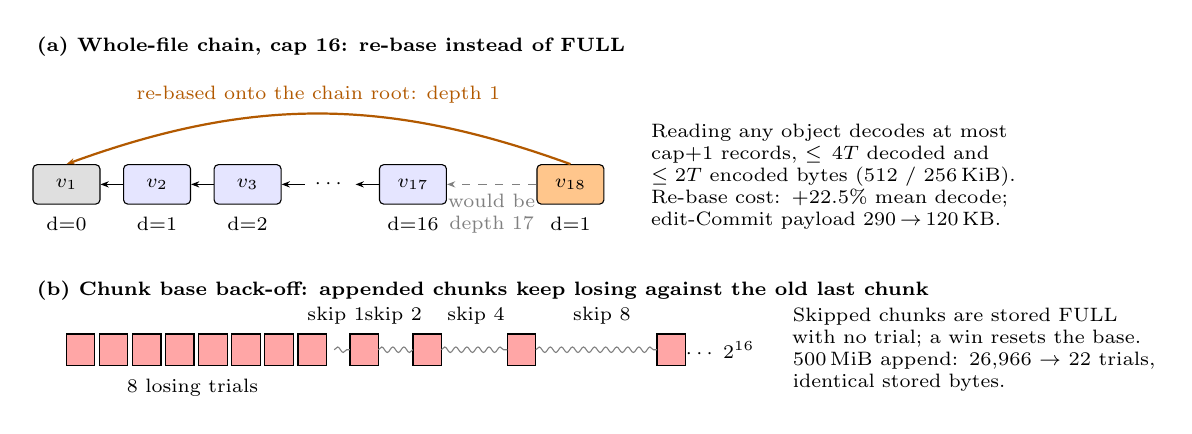
\begin{tikzpicture}[font=\scriptsize,
  ob/.style={draw, rounded corners=1.5pt, minimum width=0.85cm, minimum height=0.5cm, inner sep=1pt},
  full/.style={ob, fill=gray!25},
  pre/.style={ob, fill=blue!10},
  bk/.style={-{Stealth[length=3pt]}}]
\node[font=\scriptsize\bfseries, anchor=west] at (-0.5,1.75) {(a) Whole-file chain, cap 16: re-base instead of FULL};
\node[full] (v1) at (0,0) {$v_1$};
\node[pre] (v2) at (1.15,0) {$v_2$};
\node[pre] (v3) at (2.3,0) {$v_3$};
\node (dots) at (3.35,0) {$\cdots$};
\node[pre] (v16) at (4.4,0) {$v_{17}$};
\node[pre, fill=orange!45] (v17) at (6.4,0) {$v_{18}$};
\draw[bk] (v2) -- (v1); \draw[bk] (v3) -- (v2); \draw[bk] (dots) -- (v3); \draw[bk] (v16) -- (dots);
\draw[bk, orange!70!black, thick] (v17.north) to[out=160,in=20] node[above, font=\scriptsize]{re-based onto the chain root: depth 1} (v1.north);
\draw[bk, dashed, gray] (v17) -- node[below, font=\scriptsize, align=center]{would be\\depth 17} (v16);
\foreach \n/\d in {v1/0, v2/1, v3/2, v16/16, v17/1}{\node[font=\scriptsize, below=1pt of \n] {d=\d};}
\node[anchor=west, align=left, font=\scriptsize, text width=4.6cm] at (7.3,0.1) {Reading any object decodes at most cap$+1$ records, $\leq 4T$ decoded and $\leq 2T$ encoded bytes (512 / 256\,KiB). Re-base cost: $+$22.5\% mean decode; edit-Commit payload 290\,$\rightarrow$\,120\,KB.};
% (b) back-off
\begin{scope}[yshift=-2.1cm]
\node[font=\scriptsize\bfseries, anchor=west] at (-0.5,0.75) {(b) Chunk base back-off: appended chunks keep losing against the old last chunk};
\foreach \i in {1,...,8}{\draw[fill=red!35] ({(\i-1)*0.42},-0.2) rectangle ++(0.36,0.4);}
\node[font=\scriptsize, below] at (1.6,-0.25) {8 losing trials};
\foreach \x/\g in {3.6/1, 4.4/2, 5.6/4, 7.5/8}{
  \draw[fill=red!35] (\x,-0.2) rectangle ++(0.36,0.4);
  \node[font=\scriptsize, above] at ({\x-0.25*\g*0.3-0.1},0.2) {skip \g};}
\draw[gray, decorate, decoration={snake, amplitude=1pt, segment length=4pt}] (3.4,0) -- (3.6,0);
\draw[gray, decorate, decoration={snake, amplitude=1pt, segment length=4pt}] (3.96,0) -- (4.4,0);
\draw[gray, decorate, decoration={snake, amplitude=1pt, segment length=4pt}] (4.76,0) -- (5.6,0);
\draw[gray, decorate, decoration={snake, amplitude=1pt, segment length=4pt}] (5.96,0) -- (7.5,0);
\node at (8.3,0) {$\cdots\;2^{16}$};
\node[anchor=west, align=left, font=\scriptsize, text width=4.6cm] at (9.1,0) {Skipped chunks are stored FULL with no trial; a win resets the base. 500\,MiB append: 26,966 $\rightarrow$ 22 trials, identical stored bytes.};
\end{scope}
\end{tikzpicture}
}
\caption{Bounding delta work. (a) A whole-file object that would exceed the depth cap is delta-encoded against the chain root instead of being stored FULL. (b) A chunk base that keeps losing is skipped for exponentially growing gaps.}
\label{fig:deltachain}
\end{figure}

\subsection{Exact reuse and chain reads}

Objects reach storage in waves. Duplicate identifiers within a wave are compared byte for
byte. An identifier already located with the same role and canonical length is reused
without reading it back; integrity is deferred to the read path. Concurrent writers are
arbitrated by insert-if-absent locators, and a losing writer compares its bytes with the
winner's (a mismatch is a collision error). Reading an object resolves its delta chain
iteratively, rejects cycles and chains longer than the role's cap, enforces the decoded
and encoded budgets, reconstructs base first, and authenticates every element against
its identifier.

\subsection{Commit}

\begin{algorithm}[h]
\caption{Commit of a \ws{}}
\label{alg:commit}
\small
\begin{algorithmic}[1]
\Function{Commit}{$\mathit{ws}, \mathit{force}$}
  \If{another Commit of $\mathit{ws}$ is in flight} \Return \texttt{Busy} \EndIf
  \If{no dirty rows, no pending merge, and head and base unchanged since bind} \Return \texttt{UpToDate} \EndIf
  \State $G \gets$ \Call{Capture}{} \Comment{seal generation; no row copied}
  \State producer thread: construct changed inodes of $G$ over the immutable base $\rightarrow$ bounded queue (32 batches) $\rightarrow$ Save
  \State $\mathit{cur} \gets$ head; \textbf{if} $\mathit{cur}$ moved and $\neg\mathit{force}$ \textbf{then} $\mathit{root} \gets$ \Call{Merge}{bound root, candidate, $\mathit{cur}$}
  \State Save.finish; validate; prepare install
  \State \textbf{acquire publication lane}
  \State \quad $\mathit{now} \gets$ head; \textbf{if} $\mathit{now} \neq \mathit{cur}$ \textbf{then} $\mathit{root} \gets$ \Call{Merge}{$\mathit{cur}$, $\mathit{root}$, $\mathit{now}$} bounded to 1,024 inodes
  \State \quad \textbf{if} conflicted: install merged tree with markers as local base; publish nothing
  \State \quad \textbf{else} one write transaction: check expected head, insert Commit, advance Branch
  \State \textbf{release lane}; install new base; retire $G$ after the reply
\EndFunction
\end{algorithmic}
\end{algorithm}

Capture is $O(1)$. Construction and Save work is proportional to the captured changes.
The lane holds two head reads, an optional merge of at most 1,024 changed inodes with
byte comparison capped at 1\,MiB per file, and one write transaction, independent of
tree size, history length and Branch count.

\subsection{Three-way merge and byte equality}

Merge walks the inode-table difference between the base and one side in windows of 256
\emph{serials}, not paths, so a move on one side and an edit on the other compose (the
edit lands at the new path). For an inode changed on both sides it decides in order:
identical change or one side unchanged; a \texttt{/.lww} rule (newer modification time
wins, ours on a tie); a three-way line merge for text files up to 1\,MiB, with
Git-compatible marker blocks per conflicting hunk; ours for binaries (recorded as a
conflict); kept side wrapped in deletion markers for modify/delete; and a type conflict
otherwise. The inode-table difference reads only pages whose child identifiers differ.

Because localized edits make a file's root depend on its edit history, equal bytes can
have different roots, so ``same'' means same bytes. Byte equality walks both files'
extent cursors, skips extents that are identical in chunk, offset, length and position
without reading them, and compares only the remaining ranges in 256\,KiB windows with
early exit.

% ---------------------------------------------------------------------------
\IfFileExists{appendix-analysis.tex}{% Input by appendix.tex. Numbers: notes/E-evaluation.md, notes/appendix/P-pipeline.md.
\section{Time and Storage Analysis}
\label{app:analysis}

This appendix derives the time and storage cost of each operation from the structures
in Appendices~\ref{app:objects}--\ref{app:algorithms} and checks each bound against
measurements. Measurements come from the evaluation's campaigns
(Section~\ref{sec:eval}). Each is one sample unless noted; storage bytes are exact and
times are wall clock.

\paragraph{Notation.} A tree has $N$ inodes. A file has length $F$ and $C \approx
F/\bar{c}$ chunks, with measured mean chunk size $\bar{c} \approx 19$\,KB. Pages hold at
most $P = 8$\,KiB. The mapping tree of a file has height $h_F = \lceil \log_{64} C \rceil$
or less (3 for 500\,MiB), the inode table $h_N = O(\log_{50} N)$, and a directory with $D$
entries $h_D = O(\log D)$. A Commit captures a set $\Delta$ of changed inodes; changed
file $i$ received $w_i$ written bytes in $e_i$ separate edit runs. $T$ is the whole-file
cutoff (128\,KiB). $H$ is history length and $B$ the number of Branches.

\subsection{Time}

\begin{table}[h]
\centering
\small
\begin{tabular}{p{0.15\linewidth} p{0.30\linewidth} p{0.17\linewidth} p{0.28\linewidth}}
\toprule
Operation & Cost & Grows with & Measured (median) \\
\midrule
Mount & Template copy $+$ one root object & nothing & 17--43\,ms across machines \\
WRITE $w$ & $O(w + \log R)$ overlay rows; no Store I/O & $w$ & -- \\
READ $w$, cold & $O(w + h_F + h_N)$ pages; $\leq$ cap$+1$ records and $\leq 4T$ decoded per object & $w$; $\log F$, $\log N$ & 158\,MB/s large file; flat across history ($<$1\%) \\
Capture & Generation flip & nothing & -- \\
Commit, construction & $O\big(\sum_{i\in\Delta}(w_i + e_i h_F P) + |\Delta| h_N P\big)$ & changes only & 100\,B edit: 24.4 / 24.5 / 28.1\,ms at 10 / 100 / 500\,MiB \\
Commit, lane & 2 head reads, $\leq$1,024-inode merge, one transaction & nothing ($N$, $H$, $B$) & no-change Commit 15--21\,ms \\
Commit, new data & $O(w)$ chunking, hashing, zstd, packing & $w$ & 500\,MiB: 1.36\,s ($\approx$385\,MB/s) \\
Fork & One Branch row & nothing & -- \\
Merge & Pages whose child ids differ, windows of 256 serials; $\leq$1\,MiB byte compare per text file & changed serials & -- \\
Unmount & Drain, close, delete overlay file & open state & 14--31\,ms \\
\bottomrule
\end{tabular}
\caption{Time per operation. Mount, Commit and unmount times are CLI calls including
process launch and routing, which costs 26--54\,ms alone; the Commit times are cold.}
\label{tab:time}
\end{table}

\paragraph{File size does not enter a Commit.} A localized edit touches one
root-to-boundary path per edit boundary, so its construction cost is $O(w + e\,h_F P)$,
and $h_F$ grows by one level per 64--128$\times$ growth in $F$. A 50$\times$ increase in
file size (10 to 500\,MiB) raised the cold Commit of a 100\,B overwrite from 24.4 to
28.1\,ms; a copy-up overlay grew from 191 to 604\,ms over the same range, and its time is
$\Theta(F)$. In a unit test the same three-extent overwrite read 3 mapping pages on an
8\,MB file and 4 on a 24\,MB file.

\paragraph{Tree size, history and Branch count do not enter the lane.} The publication
lane holds two head reads, a merge bounded to 1,024 inodes, and one transaction that
inserts a Commit and advances one Branch head. None of these reads the tree beyond the
bounded merge, walks history or enumerates Branches. Work that does grow---capture of
large changes, construction, compression, pack writes, and a full merge when the head
has moved---runs before the lane, so concurrent Commits overlap in all of it
(Figure~\ref{fig:twocommits}).

\paragraph{Reads are bounded by structure, not history.} A cold read of $w$ bytes costs
$O(w)$ plus one root-to-leaf path in the inode table and in the file's mapping tree. Each
stored object resolves a delta chain of at most 16 (whole file) or 8 (chunk) records,
decoding at most $4T = 512$\,KiB and reading at most $2T = 256$\,KiB encoded; a chain
that would exceed these bounds is re-based onto its root when written. Reads of a 65\,MB
tree and of a 500\,MiB file were within 1\% of each other before and after 40 and 5
Commits of history. Large-file reads are slow in absolute terms (158\,MB/s cold against
943\,MB/s for ovnfs) because each 128\,KiB FUSE request is a round trip with one
background request outstanding; that is a kernel-route cost, not a history cost.

\paragraph{Per-call overhead.} For per-tool-call \ws{}s, the cost added to each call is
mount, Commit and unmount. On a Docker machine with a SQLite Store the clean tiny-workload
row measured 19.2, 16.0 and 16.8\,ms, about 52\,ms in all with process launch included.
Sandbox creation is separate and amortized over many calls: 0.39\,s median on Docker,
44--68\,ms natively on macOS and in Apple containers. File calls that need no process
pay neither, because they run in the SDK's process (Section~\ref{sec:filecalls}).

\paragraph{Where time is lost.} New data is written twice, once into the overlay and
again into the Store, so a 500\,MiB random write committed in 1.36\,s against 1.0\,s for
a copy-up overlay. FUSE publication of every \texttt{write(2)} makes write bandwidth a
small fraction of a kernel overlay's (Appendix~\ref{app:modal}). Large files saved under
a new inode are re-chunked in full at Commit.

\subsection{Storage}

\begin{figure}[h]
\centering
\resizebox{\linewidth}{!}{% Measured time and storage. Input by appendix-analysis.tex.
\begin{tikzpicture}
\begin{groupplot}[group style={group size=3 by 1, horizontal sep=1.55cm},
  width=5.9cm, height=4.6cm,
  tick label style={font=\tiny}, label style={font=\scriptsize}, title style={font=\scriptsize\bfseries},
  legend style={font=\tiny, draw=none, fill=none}, ymode=log, grid=major, grid style={gray!20}]
% (a) Commit time vs file size
\nextgroupplot[title={(a) Cold Commit, 100\,B overwrite}, xmode=log, xlabel={file size (MiB)}, ylabel={ms},
  xtick={10,100,500}, xticklabels={10,100,500}, ymin=10, ymax=1000, legend pos=north west]
\addplot[mark=square*, orange!80!black, thick] coordinates {(10,190.9) (100,221.1) (500,603.9)};
\addlegendentry{copy-up (ovnfs)}
\addplot[mark=*, blue!70!black, thick] coordinates {(10,24.4) (100,24.5) (500,28.1)};
\addlegendentry{\sys{}}
% (b) store growth per Commit
\nextgroupplot[title={(b) Store growth per Commit}, ybar, bar width=4pt, ylabel={bytes},
  symbolic x coords={L10,L100,L500,I10,A5,DEL500}, xtick=data, x tick label style={rotate=40, anchor=east, font=\tiny},
  ymin=1e3, ymax=1e12, legend pos=north west, enlarge x limits=0.12]
\addplot[fill=orange!60, draw=orange!80!black] coordinates {(L10,10.5e6) (L100,104.9e6) (L500,524.3e6) (I10,10.5e6) (A5,613e3) (DEL500,524.3e6)};
\addlegendentry{copy-up (ovnfs)}
\addplot[fill=blue!40, draw=blue!70!black] coordinates {(L10,5.5e3) (L100,5.3e3) (L500,7.4e3) (I10,5.3e3) (A5,18.4e3) (DEL500,8.2e3)};
\addlegendentry{\sys{}}
% (c) logical / stored
\nextgroupplot[title={(c) Logical $\div$ stored bytes}, xbar, bar width=5pt, xmode=log, ymode=normal,
  symbolic y coords={M01 tiny files,M08 SQLite DB,D10 repo replay,M02 tree copies,D03 repo replay,M03 text edits,H05 20 projects,H01 500 Commits},
  ytick=data, y tick label style={font=\tiny}, xmin=0.5, xmax=4000, xlabel={ratio (SQLite Store)},
  nodes near coords, nodes near coords style={font=\tiny, anchor=west}, point meta=explicit symbolic,
  enlarge y limits=0.08]
\addplot[fill=blue!40, draw=blue!70!black] coordinates {
 (0.91,M01 tiny files) [0.91] (13.73,M08 SQLite DB) [13.7] (11.71,D10 repo replay) [11.7] (16.97,M02 tree copies) [17.0]
 (27.48,D03 repo replay) [27.5] (29.27,M03 text edits) [29.3] (275.5,H05 20 projects) [276] (1225.9,H01 500 Commits) [1226]};
\end{groupplot}
\end{tikzpicture}
}
\caption{Measured time and storage. (a) Cold Commit time of a 100\,B overwrite is flat in file size for \sys{} and grows with it for a copy-up overlay. (b) Store growth per Commit for large-file edits (log scale; DEL500 truncates 500\,MiB). (c) Logical snapshot bytes over stored bytes across workloads; tiny files are the one case where the Store is larger than the data.}
\label{fig:charts}
\end{figure}

\paragraph{Cost of one change.} Store growth from a Commit is new payload plus new
metadata plus pack and locator overhead. Unchanged files, chunks, pages and subtrees
cost nothing, because identities are content hashes and updates rewrite only paths to
changes.
\begin{itemize}[leftmargin=*,nosep]
\item \emph{Payload.} A localized edit of $w$ bytes in a chunked file creates between
$\lceil w/32\,\mathrm{KiB}\rceil$ and $\lceil w/8\,\mathrm{KiB}\rceil + 1$ new chunks,
because only the replacement is chunked and boundary chunks become slices of existing
chunks. Payload is therefore at most $w$ plus per-record framing (or a smaller delta),
independent of $F$. A 100\,B random overwrite stored 153\,B of payload at 10, 100 and
500\,MiB. A small file ($< T$) is rewritten whole, so its payload is a delta against
the previous version, bounded by its compressed size.
\item \emph{Metadata.} A changed file rewrites at most $h_F$ mapping pages, a 93\,B file
state, $h_N$ inode-table pages and a 116\,B root; a name change also rewrites $h_D$
directory pages. Canonically this is $O((h_F + h_N + h_D)P)$, 17--26\,KB for a
mid-file overwrite of a large file. Each rewritten page is stored as a COPY/INSERT
program against the page it replaces, so 3.7--5.7\,KB is stored. Across mixed histories
a least-squares fit gives 414\,B per edit, 526\,B per append, 464\,B per rename,
1,111\,B per delete and 1,360\,B per new file.
\item \emph{Store overhead.} SQLite pages, locators and indexes add 1--20\% over the
stored records (1.01--1.20\X{}; PostgreSQL 1.05--1.39\X{}). Per object the floor is
about 200\,B, which dominates only for tiny files.
\end{itemize}

\begin{table}[h]
\centering
\small
\begin{tabular}{p{0.32\linewidth} p{0.20\linewidth} p{0.38\linewidth}}
\toprule
Change & Cost bound & Measured \\
\midrule
100\,B overwrite of a 500\,MiB file & $O(w + h_F P)$ & 7.4\,KB growth per Commit (copy-up overlay: 524.3\,MB) \\
16\,KiB append to a 5\,MiB file & $O(w)$ & 18.4\,KB per Commit (613\,KB) \\
Truncate 500\,MiB off a 1,000\,MiB file & $O(h_F P)$ & 8.2\,KB (524.3\,MB) \\
Remove a 500\,MiB file & $O(h_N P)$ & 24.6\,KB; frees nothing \\
Copy a 50\,MB tree 10 times & $O(\text{metadata})$ & 15.9\,KB per copy Commit, 0 payload \\
Fork a Branch & one row; first Commit pays its paths & 5.4\,KB per identical Branch \\
Second project in a shared Store & $O(\text{metadata})$ for shared content & 220\,KB per Init (first: 23.6\,MB) \\
Commit in a 65\,MB tree (5 mixed ops) & $O(\sum$ changes$)$ & 5.9\,KB growth per Commit over 500 Commits \\
\bottomrule
\end{tabular}
\caption{Store growth per change. Copy-up figures are ovnfs on the same host.}
\label{tab:storagechange}
\end{table}

\paragraph{Cost of a history.} Store size after $k$ Commits is the initial tree plus
the sum of per-change costs; it does not grow with the size of each snapshot. Over 500
Commits on a 65\,MB tree (32.5\,GB of logical snapshots) the Store reached 26.5\,MB:
23.6\,MB of initial tree plus 5.9\,KB per Commit, a ratio of 1,226\X{} between logical
and stored bytes. Table~\ref{tab:ksnap} compares the growth of $k$ snapshots in which
each snapshot changes $m$ files of size $F$ by $w$ bytes. Copy-up overlays and
whole-file snapshot images grow with $F$; block copy-on-write grows with the touched
blocks, but has no cross-file deduplication or deltas; \sys{} grows with $w$ plus a
logarithmic path. A fully repacked Git pack is the tightest point of reference---1.10 to
1.31\X{} smaller on the measured histories, because one global repack deltas across all
versions---but Git keeps no live mountable view and must repack to reach that size.

\begin{table}[h]
\centering
\small
\begin{tabular}{p{0.30\linewidth} p{0.27\linewidth} p{0.33\linewidth}}
\toprule
System & Growth for $k$ snapshots & Measured point \\
\midrule
Copy-up overlay; whole-file snapshot images & $k\,m\,F$ & 100\,B edits to 100\,MiB file: 1.15\,GB after 10 \\
Block copy-on-write (Btrfs, ImageFS-blk) & $k\,m\,\lceil w/b\rceil b$ $+$ metadata & 4\,KiB change to 512\,MiB file: about 36\,KiB (Btrfs; recovered report) \\
Git after full repack & $\approx k\,m\,\delta(w)$, after repack & 1.10--1.31\X{} smaller than \sys{} \\
\sys{} & $k\,(m(w + c\,h_F P') + h_N P')$ & same 10 edits: 106.3\,MB, of which 104.9\,MB is the initial file \\
\bottomrule
\end{tabular}
\caption{Growth over $k$ snapshots. $b$ is the block size, $\delta(w)$ a delta of $w$
bytes, and $P'$ the stored size of a page program.}
\label{tab:ksnap}
\end{table}

\paragraph{Trade-offs taken.} Several storage choices were made, or refused, on their
time cost, following the rule that a large speed loss is not traded for a small storage
gain (Table~\ref{tab:tradeoffs}).

\begin{table}[h]
\centering
\small
\begin{tabular}{p{0.30\linewidth} p{0.30\linewidth} p{0.30\linewidth}}
\toprule
Choice & Time effect & Storage effect \\
\midrule
Re-base at the chain bound & $+$22.5\% mean decode; max 520,575\,B $\leq$ 4$T$ budget & Edit Commit payload 290\,KB $\rightarrow$ 120\,KB \\
Losing-base back-off & 500\,MiB append: 26,966 $\rightarrow$ 22 trials, 7.9 $\rightarrow$ 5.5\,s & Identical bytes \\
Win saving $<$1/8 counts as loss & 100\,MiB log append 1,540 $\rightarrow$ 977\,ms & $+$1.04\% stored \\
zstd-3, not zstd-6 (refused) & zstd-6 costs 2.6\X{} compression CPU & zstd-6 would save 4.4\% \\
Per-object records, no group compression (refused) & Group: decode 256\,KiB to serve 2\,KB & Group would save 22\% \\
Per-chunk frames & Random-access reads & Text 1.25\X{} larger than whole-file zstd \\
No garbage collection or repack & No background work & Deleted data is retained \\
\bottomrule
\end{tabular}
\caption{Speed and storage trade-offs, from the design records.}
\label{tab:tradeoffs}
\end{table}
}{}

% ---------------------------------------------------------------------------
\section{Comparison with Image-FUSE and Overlayfs Sandboxes}
\label{app:modal}

Agent sandboxes commonly build their root filesystem from a lazily loaded, read-only
image and a writable copy-on-write layer. Modal's design is a well-documented example
with two generations~\cite{modalvmfs,modalimagefs,modallaunch}. \emph{ImageFS} serves
images through a FUSE server backed by a whole-file content-addressed cache spanning
memory, local SSD, zonal caches, a CDN and blob storage, with a kernel overlayfs upper on
XFS above it; whole-file copy-up in that arrangement can, in Modal's words, cost
gigabytes of overhead to write individual bytes. For VM sandboxes, Modal reports that
exposing this stack over virtio-fs made metadata-heavy work several times slower
(recursive \texttt{chown} from about 4\,s to over a minute) and replaced it with
\emph{ImageFS-blk}: the host synthesizes a sparse ext4 image, serves its blocks lazily
over virtio-blk, and records guest writes block by block in a per-VM sparse file with a
dirty bitmap, so the guest kernel owns all metadata~\cite{modalvmfs,modalvm}. Snapshots
are exposed as images that store the modified files, with an alpha memory snapshot that
also captures processes; filesystem snapshots expire after 30 days by default and cannot
be listed~\cite{modalsnap}. Table~\ref{tab:modal} compares the designs.

\begin{table}[h]
\centering
\small
\begin{tabular}{p{0.14\linewidth} p{0.24\linewidth} p{0.24\linewidth} p{0.26\linewidth}}
\toprule
& FUSE image $+$ overlayfs & Block image (ImageFS-blk) & \sys{} \\
\midrule
Lower layer & Read-only image, whole-file content addressing & Synthesized sparse ext4 image & Any committed root of any Branch \\
Lazy-load unit & Whole file; 32\,MB read-ahead & Block, mapped to file ranges & Tree page, whole file $<$128\,KiB, 8--32\,KiB chunk; authenticated \\
Write target & overlayfs upper on XFS & Per-VM sparse file, dirty bitmap & Per-\ws{} SQLite overlay \\
Copy-up unit & Whole file & One block & None: 4\,KiB cells; references for unchanged chunks \\
Metadata ops & Copy-up of lower files unless \texttt{metacopy} & In guest (\texttt{chown} $\approx$2\,\textmu s) & One overlay row; one FUSE round trip \\
Snapshot output & Image of modified files & Image of modified files (dirty bitmap) & Immutable Commit; chunk dedup and deltas \\
Snapshot cost & $\propto$ bytes of modified files & Not published & $\propto$ changed paths and bytes \\
Fork, history, merge & New sandbox from image; no history & Same & Fork is one row; diff, merge, blame \\
Distribution & Fleet-wide cache tiers & Fleet-wide cache tiers & One Store (one kernel, or PostgreSQL) \\
Steady-state I/O & Kernel page cache and overlayfs & Guest ext4 and page cache & FUSE; write-back off; 128\,KiB requests \\
POSIX coverage & Full & Full (Docker inside the VM) & No xattrs, FIFOs, locks, \texttt{fallocate} \\
\bottomrule
\end{tabular}
\caption{Image-based sandbox filesystems and \sys{}. Modal entries are taken from its
publications and documentation, not reproduced.}
\label{tab:modal}
\end{table}

\begin{figure}[h]
\centering
\resizebox{\linewidth}{!}{% What a 100-byte overwrite of a 500 MiB file costs in three designs. Input by appendix.tex.
\begin{tikzpicture}[font=\scriptsize, x=1cm, y=1cm,
  lbl/.style={anchor=east, align=right, text width=2.9cm},
  note/.style={anchor=west, align=left, font=\scriptsize, text width=5.0cm}]
\def\W{7.0}
% lower layer, common
\node[lbl] at (-0.2,0) {committed file (500\,MiB)};
\draw[fill=gray!15] (0,-0.2) rectangle (\W,0.2);
\draw[red!70!black, very thick] (4.55,-0.3) -- (4.55,0.3);
\node[font=\scriptsize, red!70!black, above] at (4.55,0.3) {100\,B write};
% copy-up overlay
\node[lbl] at (-0.2,-1.0) {copy-up overlay\\(overlayfs upper, ovnfs)};
\draw[fill=orange!55] (0,-1.2) rectangle (\W,-0.8);
\node[font=\scriptsize] at (\W/2,-1.0) {whole file copied up before the write};
\node[note] at (\W+0.2,-1.0) {write: 500\,MiB copy\\snapshot: 524.3\,MB, 0.6\,s per Commit};
% block CoW
\node[lbl] at (-0.2,-2.0) {block copy-on-write\\(ImageFS-blk, Btrfs)};
\draw[fill=gray!15] (0,-2.2) rectangle (\W,-1.8);
\draw[fill=orange!55] (4.5,-2.2) rectangle (4.65,-1.8);
\node[font=\scriptsize, anchor=west] at (4.7,-2.0) {one 4\,KiB block};
\node[note] at (\W+0.2,-2.0) {write: one block\\snapshot: modified \emph{file} in Modal;\\$\approx$36\,KiB extent in Btrfs};
% LayerFS
\node[lbl] at (-0.2,-3.0) {\sys{} overlay};
\draw[dotted] (0,-3.2) rectangle (\W,-2.8);
\draw[fill=orange!55] (4.5,-3.2) rectangle (4.65,-2.8);
\node[font=\scriptsize, anchor=west] at (4.7,-3.0) {one 4\,KiB cell};
\node[font=\scriptsize] at (2.0,-3.0) {nothing else stored};
\node[note] at (\W+0.2,-3.0) {write: one cell row (100\,B valid),\\no base read};
\node[lbl] at (-0.2,-4.0) {\sys{} Commit};
\draw[fill=gray!15] (0,-4.2) rectangle (\W,-3.8);
\foreach \x in {0.8,1.6,2.5,3.2,3.9,5.3,6.1}{\draw[gray] (\x,-4.2) -- (\x,-3.8);}
\draw[fill=gray!15, pattern=north east lines, pattern color=gray] (3.9,-4.2) rectangle (5.3,-3.8);
\draw[fill=orange!55] (4.5,-4.2) rectangle (4.65,-3.8);
\node[font=\scriptsize, anchor=north] at (4.65,-4.25) {old chunk $\rightarrow$ two slices $+$ new 100\,B chunk};
\node[font=\scriptsize, fill=gray!15, inner sep=1pt] at (1.9,-4.0) {other chunks shared};
\node[note] at (\W+0.2,-4.0) {Commit: 153\,B payload $+$ path pages\\snapshot: 7.4\,KB, 28\,ms per Commit};
\end{tikzpicture}
}
\caption{What a 100\,B overwrite of a 500\,MiB file costs at write time and at snapshot time in each design. Copy-up and Commit figures are measured on one host; block copy-on-write figures are from Modal's description and a recovered Btrfs report.}
\label{fig:comparison}
\end{figure}

\paragraph{Where \sys{} wins.} The differences that matter for agents are in capture and
history. \sys{} never copies up: a 100\,B edit to a 500\,MiB file commits in 20--28\,ms
and adds 3--8\,KB, whereas a whole-file copy-up overlay (ovnfs, measured on the same
host) took about 0.6\,s and stored a full copy; across ten such edits to a 100\,MiB file
\sys{} stores 106\,MB against 1.15\,GB (Table~\ref{tab:ovnfs}). Against block-level
copy-on-write the write-time advantage largely disappears, but the snapshot difference
remains: Modal's documented snapshot unit is the modified file, so a database, a Git
pack or a build artifact touched by one byte is captured whole, and there is no
branch, merge, diff or history. In \sys{} every step is a Commit, forks are one row,
and unchanged chunks, pages and subtrees are shared across Commits, Branches and
projects.

\paragraph{Where \sys{} loses.} Raw I/O and coverage favor the image designs. Every
\sys{} write is a FUSE request published to SQLite before it returns, and the mount
negotiates 128\,KiB read-ahead with one background request. In an earlier three-way
measurement on the same host (a v1.0-era build, warm, one sample), kernel overlayfs
achieved 6\X{} the sequential-write and 75\X{} the 4\,KiB random-write bandwidth of
\sys{} and created small files 30\X{} faster; cold sequential reads of a 500\,MiB file
reach 158\,MB/s against 943\,MB/s for another FUSE overlay and about 2.5\,GiB/s that
Modal reports for ImageFS with 32\,MB read-ahead. ImageFS-blk performs metadata
operations entirely in the guest. \sys{} omits extended attributes, special files, locks
and \texttt{fallocate}, so Docker-in-sandbox, which Modal's VM runtime targets, cannot
run on a \ws{}. Modal distributes images across a fleet, while a \sys{} SQLite Store is
confined to one kernel.

\paragraph{Complementary, not competing.} The comparison is not a single ordering:
\sys{} is better at the operations that make sandbox state versioned---commit cost
proportional to change, sub-file copy-on-write, deduplication across snapshots, cheap
forks and history---and worse at steady-state throughput, POSIX coverage and fleet-scale
distribution. The designs also compose: a \sys{} \ws{} can run inside a VM whose block
device serves the operating system image, with \sys{} serving only the project. A fair
evaluation would run, on one native Linux host, \sys{}, a FUSE-image lower with an
overlayfs upper and whole-file snapshots, a block-level copy-on-write analog of
ImageFS-blk, and plain ext4, on (1) per-tool-call agent replays with a snapshot after
each mutating call, (2) small edits to 10\,MiB--1\,GiB files, a SQLite database and a
large Git repository, (3) Modal's own metadata and install workloads, (4) fork fan-out
to 64 views, and (5) 1,000 sequential snapshots, plus (6) a \sys{} ablation of
read-ahead, background requests and write-back caching that separates design cost from
tuning.

% ---------------------------------------------------------------------------
\IfFileExists{appendix-cli.tex}{% CLI reference appendix, generated from the 2.0 call table
% (origin/layerfs_v2_0_0 at 8cfb6e2734, api/crates/layerfs-api/src/<family>/<call>.rs).
% Source list: notes/cli-calls.md.
\section{Command-Line Interface}
\label{app:cli}

\sys{} 2.0 exposes one call table: 73 calls in ten families. The \texttt{layerfs}
command, the Node SDK and the Python SDK are all generated from it, so
\texttt{layerfs file write} on the command line is \texttt{layerfs.file.write} in the
SDKs, with the same positional arguments and options. Positionals run from the
outside in: owner, Branch, path or new name, other inputs, and an optional Commit
last. A project is named \texttt{<store>/<project>}. File content comes from standard
input or \texttt{--from}. Every call prints JSON, or text with \texttt{--text}; it exits
0 when done, 2 on a malformed command line and 125 when refused, with a structured
\texttt{\{code, message, detail\}} on standard error. Each call is attempted once and
never retried. Table~\ref{tab:cli} lists every call; five more commands exist only on
the command line (\texttt{help}, \texttt{--version}, \texttt{doctor},
\texttt{import-env} and \texttt{worker}).

{\footnotesize
\setlength{\LTpre}{4pt}\setlength{\LTpost}{0pt}
\begin{longtable}{@{}p{0.60\linewidth}@{\hspace{1em}}p{0.36\linewidth}@{}}
\caption{Every call of the \sys{} 2.0 command line, generated from the call table.
\texttt{[...]} marks an optional positional or option.}\label{tab:cli}\\
\toprule
Command & What it does \\
\midrule
\endfirsthead
\toprule
Command & What it does \\
\midrule
\endhead
\bottomrule
\endfoot
\multicolumn{2}{@{}l}{\textbf{Stores} (12)}\\*
{\raggedright\ttfamily layerfs store attach \textless{}name\textgreater{} \textless{}machine\textgreater{} [--url \textless{}url\textgreater{}] [--password \textless{}password\textgreater{}]} & Let a machine run Sandboxes of a PostgreSQL Store, after checking it reaches the server \\
{\raggedright\ttfamily layerfs store connect \textless{}name\textgreater{} \textless{}url\textgreater{} [--password \textless{}password\textgreater{}] [--synchronous-commit \textless{}synchronous-commit\textgreater{}]} & Attach a PostgreSQL database as a Store \\
{\raggedright\ttfamily layerfs store create \textless{}name\textgreater{}} & An empty sqlite Store on native \\
{\raggedright\ttfamily layerfs store detach \textless{}name\textgreater{} \textless{}machine\textgreater{}} & Stop a machine running Sandboxes of a PostgreSQL Store \\
{\raggedright\ttfamily layerfs store disconnect \textless{}name\textgreater{}} & Forget a PostgreSQL Store; its data stays \\
{\raggedright\ttfamily layerfs store get \textless{}name\textgreater{}} & A Store's record \\
{\raggedright\ttfamily layerfs store list} & Every Store, from the home's records \\
{\raggedright\ttfamily layerfs store pull \textless{}name\textgreater{} [--progress]} & Bring a sqlite Store from its machine to native \\
{\raggedright\ttfamily layerfs store push \textless{}name\textgreater{} \textless{}machine\textgreater{} [--progress]} & Send a sqlite Store from native to a machine \\
{\raggedright\ttfamily layerfs store remove \textless{}name\textgreater{}} & Delete a sqlite Store with every project in it \\
{\raggedright\ttfamily layerfs store stats \textless{}name\textgreater{}} & Store-wide publication and allocation counters \\
{\raggedright\ttfamily layerfs store status \textless{}name\textgreater{}} & A Store's live state \\
\addlinespace
\multicolumn{2}{@{}l}{\textbf{Projects} (6)}\\*
{\raggedright\ttfamily layerfs project export \textless{}project\textgreater{} \textless{}destination\textgreater{} [--branch \textless{}branch\textgreater{}] [--progress]} & Export a project's snapshot from its Store to a local folder \\
{\raggedright\ttfamily layerfs project get \textless{}project\textgreater{}} & A project's record: its Store, kind and machine \\
{\raggedright\ttfamily layerfs project init \textless{}project\textgreater{} \textless{}folder\textgreater{} [--timeout \textless{}timeout\textgreater{}] [--progress]} & Import a host folder as a new project into an existing Store \\
{\raggedright\ttfamily layerfs project list [\textless{}store\textgreater{}] [--page-size \textless{}page-size\textgreater{}] [--page-pos \textless{}page-pos\textgreater{}]} & Every project in the home, or one Store's \\
{\raggedright\ttfamily layerfs project remove \textless{}project\textgreater{}} & Remove one project from its Store \\
{\raggedright\ttfamily layerfs project stats \textless{}project\textgreater{} [\textless{}branch\textgreater{}] [\textless{}commit\textgreater{}]} & Entry counts of one pinned saved tree \\
\addlinespace
\multicolumn{2}{@{}l}{\textbf{Branches} (8)}\\*
{\raggedright\ttfamily layerfs branch commits \textless{}project\textgreater{} \textless{}branch\textgreater{} [--page \textless{}page\textgreater{}] [--page-size \textless{}page-size\textgreater{}] [--at-commit \textless{}at-commit\textgreater{}] [--include-storage]} & Saved branch commits or main publications, newest first \\
{\raggedright\ttfamily layerfs branch diff \textless{}project\textgreater{} \textless{}from-branch\textgreater{} \textless{}to-branch\textgreater{} [--paths-only] [--page-size \textless{}page-size\textgreater{}] [--page-pos \textless{}page-pos\textgreater{}] [--cursor \textless{}cursor\textgreater{}] [--page \textless{}page\textgreater{}] [--from-commit \textless{}from-commit\textgreater{}] [--to-commit \textless{}to-commit\textgreater{}] [--path-prefix \textless{}path-prefix\textgreater{}] [--include-attribution] [--continuation \textless{}continuation\textgreater{}]} & Files that differ between two Branches' heads \\
{\raggedright\ttfamily layerfs branch fork \textless{}project\textgreater{} \textless{}name\textgreater{} \textless{}from-branch\textgreater{} [\textless{}from-commit\textgreater{}]} & A new Branch from another Branch's head or Commit \\
{\raggedright\ttfamily layerfs branch get \textless{}project\textgreater{} \textless{}branch\textgreater{}} & One Branch and its head Commit \\
{\raggedright\ttfamily layerfs branch get-commit \textless{}project\textgreater{} \textless{}branch\textgreater{} \textless{}commit\textgreater{}} & One saved Commit or main publication \\
{\raggedright\ttfamily layerfs branch list \textless{}project\textgreater{} [--page-size \textless{}page-size\textgreater{}] [--page-pos \textless{}page-pos\textgreater{}] [--page \textless{}page\textgreater{}]} & A project's Branches \\
{\raggedright\ttfamily layerfs branch merge \textless{}project\textgreater{} \textless{}name\textgreater{} \textless{}a\textgreater{} \textless{}b\textgreater{} [--message \textless{}message\textgreater{}] [--units \textless{}units\textgreater{}]} & Merge two Branches into a new one \\
{\raggedright\ttfamily layerfs branch publish \textless{}project\textgreater{} \textless{}branch\textgreater{} [\textless{}commit\textgreater{}]} & A Branch's head or Commit as main's next Layer \\
\addlinespace
\multicolumn{2}{@{}l}{\textbf{Files (in-process; no Sandbox)} (15)}\\*
{\raggedright\ttfamily layerfs file apply \textless{}project\textgreater{} \textless{}branch\textgreater{} [--message \textless{}message\textgreater{}] [--from \textless{}file\textgreater{}]} & Apply a list of changes; one Commit \\
{\raggedright\ttfamily layerfs file blame \textless{}project\textgreater{} \textless{}branch\textgreater{} \textless{}path\textgreater{} [\textless{}commit\textgreater{}] [--from-line \textless{}from-line\textgreater{}] [--line-count \textless{}line-count\textgreater{}]} & The Commit of each line \\
{\raggedright\ttfamily layerfs file cp \textless{}project\textgreater{} \textless{}branch\textgreater{} \textless{}from-path\textgreater{} \textless{}to-path\textgreater{} [--message \textless{}message\textgreater{}]} & Copy a path; one Commit \\
{\raggedright\ttfamily layerfs file diff \textless{}project\textgreater{} \textless{}left-branch\textgreater{} \textless{}left-path\textgreater{} \textless{}right-branch\textgreater{} \textless{}right-path\textgreater{} [--left-commit \textless{}left-commit\textgreater{}] [--right-commit \textless{}right-commit\textgreater{}] [--include-attribution] [--allow-missing] [--page \textless{}page\textgreater{}] [--page-size \textless{}page-size\textgreater{}]} & The difference between two files \\
{\raggedright\ttfamily layerfs file edit \textless{}project\textgreater{} \textless{}branch\textgreater{} \textless{}path\textgreater{} [--old \textless{}old\textgreater{}] [--new \textless{}new\textgreater{}] [--message \textless{}message\textgreater{}]} & Replace one unique text in a file; one Commit \\
{\raggedright\ttfamily layerfs file glob \textless{}project\textgreater{} \textless{}branch\textgreater{} \textless{}path\textgreater{} \textless{}pattern\textgreater{} [\textless{}commit\textgreater{}] [--page-size \textless{}page-size\textgreater{}] [--page \textless{}page\textgreater{}] [--page-pos \textless{}page-pos\textgreater{}]} & Paths under path matching a glob \\
{\raggedright\ttfamily layerfs file grep \textless{}project\textgreater{} \textless{}branch\textgreater{} \textless{}path\textgreater{} \textless{}pattern\textgreater{} [\textless{}commit\textgreater{}] [--page-size \textless{}page-size\textgreater{}] [--page \textless{}page\textgreater{}] [--page-pos \textless{}page-pos\textgreater{}]} & Lines under path matching a regular expression \\
{\raggedright\ttfamily layerfs file list \textless{}project\textgreater{} \textless{}branch\textgreater{} \textless{}path\textgreater{} [\textless{}commit\textgreater{}] [--page-size \textless{}page-size\textgreater{}] [--page \textless{}page\textgreater{}] [--page-pos \textless{}page-pos\textgreater{}]} & A folder's entries \\
{\raggedright\ttfamily layerfs file mkdir \textless{}project\textgreater{} \textless{}branch\textgreater{} \textless{}path\textgreater{} [--message \textless{}message\textgreater{}] [--mode \textless{}mode\textgreater{}]} & Make a folder; one Commit \\
{\raggedright\ttfamily layerfs file mv \textless{}project\textgreater{} \textless{}branch\textgreater{} \textless{}from-path\textgreater{} \textless{}to-path\textgreater{} [--message \textless{}message\textgreater{}]} & Move a path; one Commit \\
{\raggedright\ttfamily layerfs file read \textless{}project\textgreater{} \textless{}branch\textgreater{} \textless{}path\textgreater{} [\textless{}commit\textgreater{}] [--start-line \textless{}start-line\textgreater{}] [--end-line \textless{}end-line\textgreater{}]} & Read a file \\
{\raggedright\ttfamily layerfs file revision \textless{}project\textgreater{} \textless{}branch\textgreater{} \textless{}path\textgreater{} [--at-commit \textless{}at-commit\textgreater{}] [--traversal \textless{}traversal\textgreater{}] [--page \textless{}page\textgreater{}] [--page-size \textless{}page-size\textgreater{}] [--continuation \textless{}continuation\textgreater{}]} & Saved changes to a literal path \\
{\raggedright\ttfamily layerfs file rm \textless{}project\textgreater{} \textless{}branch\textgreater{} \textless{}path\textgreater{} [--message \textless{}message\textgreater{}]} & Remove a path; one Commit \\
{\raggedright\ttfamily layerfs file stat \textless{}project\textgreater{} \textless{}branch\textgreater{} \textless{}path\textgreater{} [\textless{}commit\textgreater{}]} & A path's kind, size and mode \\
{\raggedright\ttfamily layerfs file write \textless{}project\textgreater{} \textless{}branch\textgreater{} \textless{}path\textgreater{} [--message \textless{}message\textgreater{}] [--mode \textless{}mode\textgreater{}] [--from \textless{}file\textgreater{}]} & Write a file; one Commit \\
\addlinespace
\multicolumn{2}{@{}l}{\textbf{Commits} (3)}\\*
{\raggedright\ttfamily layerfs commit diff \textless{}project\textgreater{} \textless{}from-commit\textgreater{} \textless{}to-commit\textgreater{} [--paths-only] [--page-size \textless{}page-size\textgreater{}] [--page-pos \textless{}page-pos\textgreater{}] [--cursor \textless{}cursor\textgreater{}]} & Files that differ between two Commits \\
{\raggedright\ttfamily layerfs commit get \textless{}project\textgreater{} \textless{}branch\textgreater{} \textless{}commit\textgreater{}} & One Commit of a Branch \\
{\raggedright\ttfamily layerfs commit list \textless{}project\textgreater{} \textless{}branch\textgreater{} [--page-size \textless{}page-size\textgreater{}] [--page-pos \textless{}page-pos\textgreater{}]} & A Branch's Commits, newest first \\
\addlinespace
\multicolumn{2}{@{}l}{\textbf{Sandboxes} (4)}\\*
{\raggedright\ttfamily layerfs sandbox close \textless{}name\textgreater{} [--force]} & Stop a Sandbox \\
{\raggedright\ttfamily layerfs sandbox create \textless{}project\textgreater{} \textless{}name\textgreater{} [\textless{}machine\textgreater{}] [--image \textless{}image\textgreater{}] [--progress]} & Start a named Sandbox of a project on a machine (default: its sqlite Store's, or native) \\
{\raggedright\ttfamily layerfs sandbox get \textless{}name\textgreater{} [--page-size \textless{}page-size\textgreater{}] [--page-pos \textless{}page-pos\textgreater{}]} & A Sandbox and its Workspaces \\
{\raggedright\ttfamily layerfs sandbox list [\textless{}project\textgreater{}] [--page-size \textless{}page-size\textgreater{}] [--page-pos \textless{}page-pos\textgreater{}]} & Every Sandbox in the home, or one project's \\
\addlinespace
\multicolumn{2}{@{}l}{\textbf{Workspaces} (6)}\\*
{\raggedright\ttfamily layerfs workspace commit \textless{}ws\textgreater{} [--message \textless{}message\textgreater{}] [--force]} & Commit a Workspace's changes to its Branch \\
{\raggedright\ttfamily layerfs workspace exec \textless{}ws\textgreater{} \textless{}command\textgreater{} [--message \textless{}message\textgreater{}] [--stream] [--exec-id \textless{}exec-id\textgreater{}] [--progress] [--events]} & Run one bash command in a Workspace \\
{\raggedright\ttfamily layerfs workspace exec-cancel \textless{}ws\textgreater{} \textless{}exec-id\textgreater{} [--grace-ms \textless{}grace-ms\textgreater{}]} & End a running command: SIGTERM, then SIGKILL after grace\_ms \\
{\raggedright\ttfamily layerfs workspace mount \textless{}sandbox\textgreater{} \textless{}branch\textgreater{} [--name \textless{}name\textgreater{}]} & Mount a Branch in a Sandbox \\
{\raggedright\ttfamily layerfs workspace status \textless{}ws\textgreater{}} & A Workspace's changes since its base \\
{\raggedright\ttfamily layerfs workspace unmount \textless{}ws\textgreater{} [--discard] [--force]} & End a Workspace \\
\addlinespace
\multicolumn{2}{@{}l}{\textbf{Machines} (12)}\\*
{\raggedright\ttfamily layerfs machine create \textless{}name\textgreater{} \textless{}platform\textgreater{} [--cpus \textless{}cpus\textgreater{}] [--memory \textless{}memory\textgreater{}] [--disk \textless{}disk\textgreater{}] [--image \textless{}image\textgreater{}] [--os-image \textless{}os-image\textgreater{}] [--progress]} & Create an enabled VM machine (apple-container, lima) \\
{\raggedright\ttfamily layerfs machine get \textless{}name\textgreater{}} & A machine's record \\
{\raggedright\ttfamily layerfs machine images \textless{}name\textgreater{}} & The Sandbox images a machine holds, and the host's Docker images it can copy \\
{\raggedright\ttfamily layerfs machine list} & Every machine, with what it supports \\
{\raggedright\ttfamily layerfs machine load \textless{}name\textgreater{} \textless{}image\textgreater{} [--progress]} & Copy an image from the host's Docker to a machine without creating a Sandbox \\
{\raggedright\ttfamily layerfs machine platforms} & The platforms this host and build support, and what each is missing \\
{\raggedright\ttfamily layerfs machine prune \textless{}name\textgreater{} [\textless{}image\textgreater{}] [--unused]} & Remove a Sandbox image from a machine, or every unused one \\
{\raggedright\ttfamily layerfs machine remove \textless{}name\textgreater{}} & Delete a VM machine and its disk; one of a removed platform is only forgotten \\
{\raggedright\ttfamily layerfs machine start \textless{}name\textgreater{} [--progress]} & Start a stopped machine and its worker; a running one answers at once \\
{\raggedright\ttfamily layerfs machine status \textless{}name\textgreater{}} & A machine's live state, free disk and tool version \\
{\raggedright\ttfamily layerfs machine stop \textless{}name\textgreater{} [--force]} & Stop a machine's worker and VM; its disks stay \\
{\raggedright\ttfamily layerfs machine update \textless{}name\textgreater{} [--cpus \textless{}cpus\textgreater{}] [--memory \textless{}memory\textgreater{}] [--image \textless{}image\textgreater{}] [--docker \textless{}docker\textgreater{}] [--wsl \textless{}wsl\textgreater{}] [--daemon \textless{}daemon\textgreater{}]} & Resize a VM, or set a built-in machine's image, Docker socket and daemon \\
\addlinespace
\multicolumn{2}{@{}l}{\textbf{Backups} (5)}\\*
{\raggedright\ttfamily layerfs backup connect \textless{}name\textgreater{} \textless{}url\textgreater{} [--key \textless{}key\textgreater{}] [--region \textless{}region\textgreater{}] [--part-size \textless{}part-size\textgreater{}]} & Connect an r2 or MinIO bucket \\
{\raggedright\ttfamily layerfs backup create \textless{}store\textgreater{} \textless{}bucket\textgreater{} [\textless{}file\textgreater{}] [--progress]} & Upload a sqlite Store to a bucket \\
{\raggedright\ttfamily layerfs backup disconnect \textless{}name\textgreater{}} & Forget a bucket and this home's links to it \\
{\raggedright\ttfamily layerfs backup list [\textless{}bucket\textgreater{}]} & Every Store file on the connected buckets \\
{\raggedright\ttfamily layerfs backup restore \textless{}store\textgreater{} \textless{}bucket\textgreater{} [\textless{}file\textgreater{}] [--progress]} & Download a backup as a sqlite Store on native \\
\addlinespace
\multicolumn{2}{@{}l}{\textbf{Call log} (2)}\\*
{\raggedright\ttfamily layerfs logs list [--op \textless{}op\textgreater{}] [--project \textless{}project\textgreater{}] [--client \textless{}client\textgreater{}] [--tag \textless{}tag\textgreater{}] [--outcome \textless{}outcome\textgreater{}] [--since \textless{}since\textgreater{}] [--cursor \textless{}cursor\textgreater{}] [--limit \textless{}limit\textgreater{}]} & The calls made against this home, newest first \\
{\raggedright\ttfamily layerfs logs reset} & Clear this home's call log \\
\addlinespace
\multicolumn{2}{@{}l}{\textbf{Command line only} (5)}\\*
{\raggedright\ttfamily layerfs help [\textless{}family\textgreater{} [\textless{}call\textgreater{}]]} & This list; \texttt{help --json} prints the call table \\
{\raggedright\ttfamily layerfs --version} & The build's version \\
{\raggedright\ttfamily layerfs doctor [--quick | --write-test] [--timeout \textless{}duration\textgreater{}]} & Report what is wrong in the home, changing nothing \\
{\raggedright\ttfamily layerfs import-env} & Write this environment's 1.1.0 settings as records, once \\
{\raggedright\ttfamily layerfs worker} & Serve this machine's worker (inside a machine) \\
\end{longtable}
}
}{}
}{}

\end{document}
